\documentclass[usenames,dvipsnames]{beamer}
\usepackage[mode=buildnew]{standalone}

\mode<presentation> {

\usetheme{Madrid}

%\setbeamertemplate{footline} % To remove the footer line in all slides uncomment this line
\setbeamertemplate{footline}[page number] % To replace the footer line in all slides with a simple slide count uncomment this line

%\setbeamertemplate{navigation symbols}{} % To remove the navigation symbols from the bottom of all slides uncomment this line
}

\usepackage{graphicx} % Allows including images
\usepackage{booktabs} % Allows the use of \toprule, \midrule and \bottomrule in tables
\usepackage{amsmath, amsfonts, amsthm, mathrsfs, bm, bbm}
\usepackage{xcolor}
\usepackage{siunitx}
\usepackage{tikz}
\usetikzlibrary{matrix,backgrounds,calc,shapes,arrows,arrows.meta,fit,positioning}
\usetikzlibrary{chains,shapes.multipart}
\usetikzlibrary{shapes,calc}
\tikzset{cross/.style={cross out, draw=black, fill=none, minimum size=2*(#1-\pgflinewidth), inner sep=0pt, outer
sep=0pt}, cross/.default={2pt}}
\usepackage{pgfplots, pgfplotstable}
\usepackage{pgfgantt}
\usepackage{varwidth}
%\pgfplotsset{compat=1.13}

\newganttchartelement*{mymilestone}{
  mymilestone/.style={
    shape=isosceles triangle,
    inner sep=0pt,
    draw=cyan,
    top color=white,
    bottom color=cyan!50
  },
  mymilestone incomplete/.style={
    /pgfgantt/mymilestone,
    draw=yellow,
    bottom color=yellow!50
  },
  mymilestone label font=\slshape,
  mymilestone left shift=0pt,
  mymilestone right shift=0pt
}

\newgantttimeslotformat{stardate}{%
\def\decomposestardate##1.##2\relax{%
\def\stardateyear{##1}\def\stardateday{##2}%
}%
\decomposestardate#1\relax%
\pgfcalendardatetojulian{\stardateyear-01-01}{#2}%
\advance#2 by-1\relax%
\advance#2 by\stardateday\relax%
}

%----------------------------------------------------------------------------------------
%	TITLE PAGE
%----------------------------------------------------------------------------------------

% The short title appears at the bottom of every slide, the full title is only on the title page
\title[Short title]{HPC-based FE$^2$ method implementation for large scale composite material problems}

\author{Student : Guido Giuntoli \\ Advisors : Mariano V\'azquez, Sergio Oller} % Your name
\institute[BSC-UPC] % Your institution as it will appear on the bottom of every slide, may be shorthand to save space
{
Barcelona Supercomputing Center\\Universitat Polit\`ecnica de Catalunya \\ % Your institution for the title page
\medskip
\textit{guido.giuntoli@bsc.es} % Your email address
}
\date{February 26, 2018} % Date, can be changed to a custom date (\today)

\begin{document}

\begin{frame}
\titlepage % Print the title page as the first slide
\end{frame}

%\begin{frame}
%\frametitle{Overview} % Table of contents slide, comment this block out to remove it
%\tableofcontents % Throughout your presentation, if you choose to use \section{} and \subsection{} commands, these will automatically be printed on this slide as an overview of your presentation
%\end{frame}

%----------------------------------------------------------------------------------------
%	PRESENTATION SLIDES
%----------------------------------------------------------------------------------------

%------------------------------------------------
%\section{First Section} % Sections can be created in order to organize your presentation into discrete blocks, all sections and subsections are automatically printed in the table of contents as an overview of the talk
%------------------------------------------------

%\subsection{Subsection Example} % A subsection can be created just before a set of slides with a common theme to further break down your presentation into chunks

%------------------------------------------------

\begin{frame}
\frametitle{Problem to solve}
\begin{figure}[!ht]
\resizebox{0.4\linewidth}{!}{\documentclass{standalone}

\begin{document}

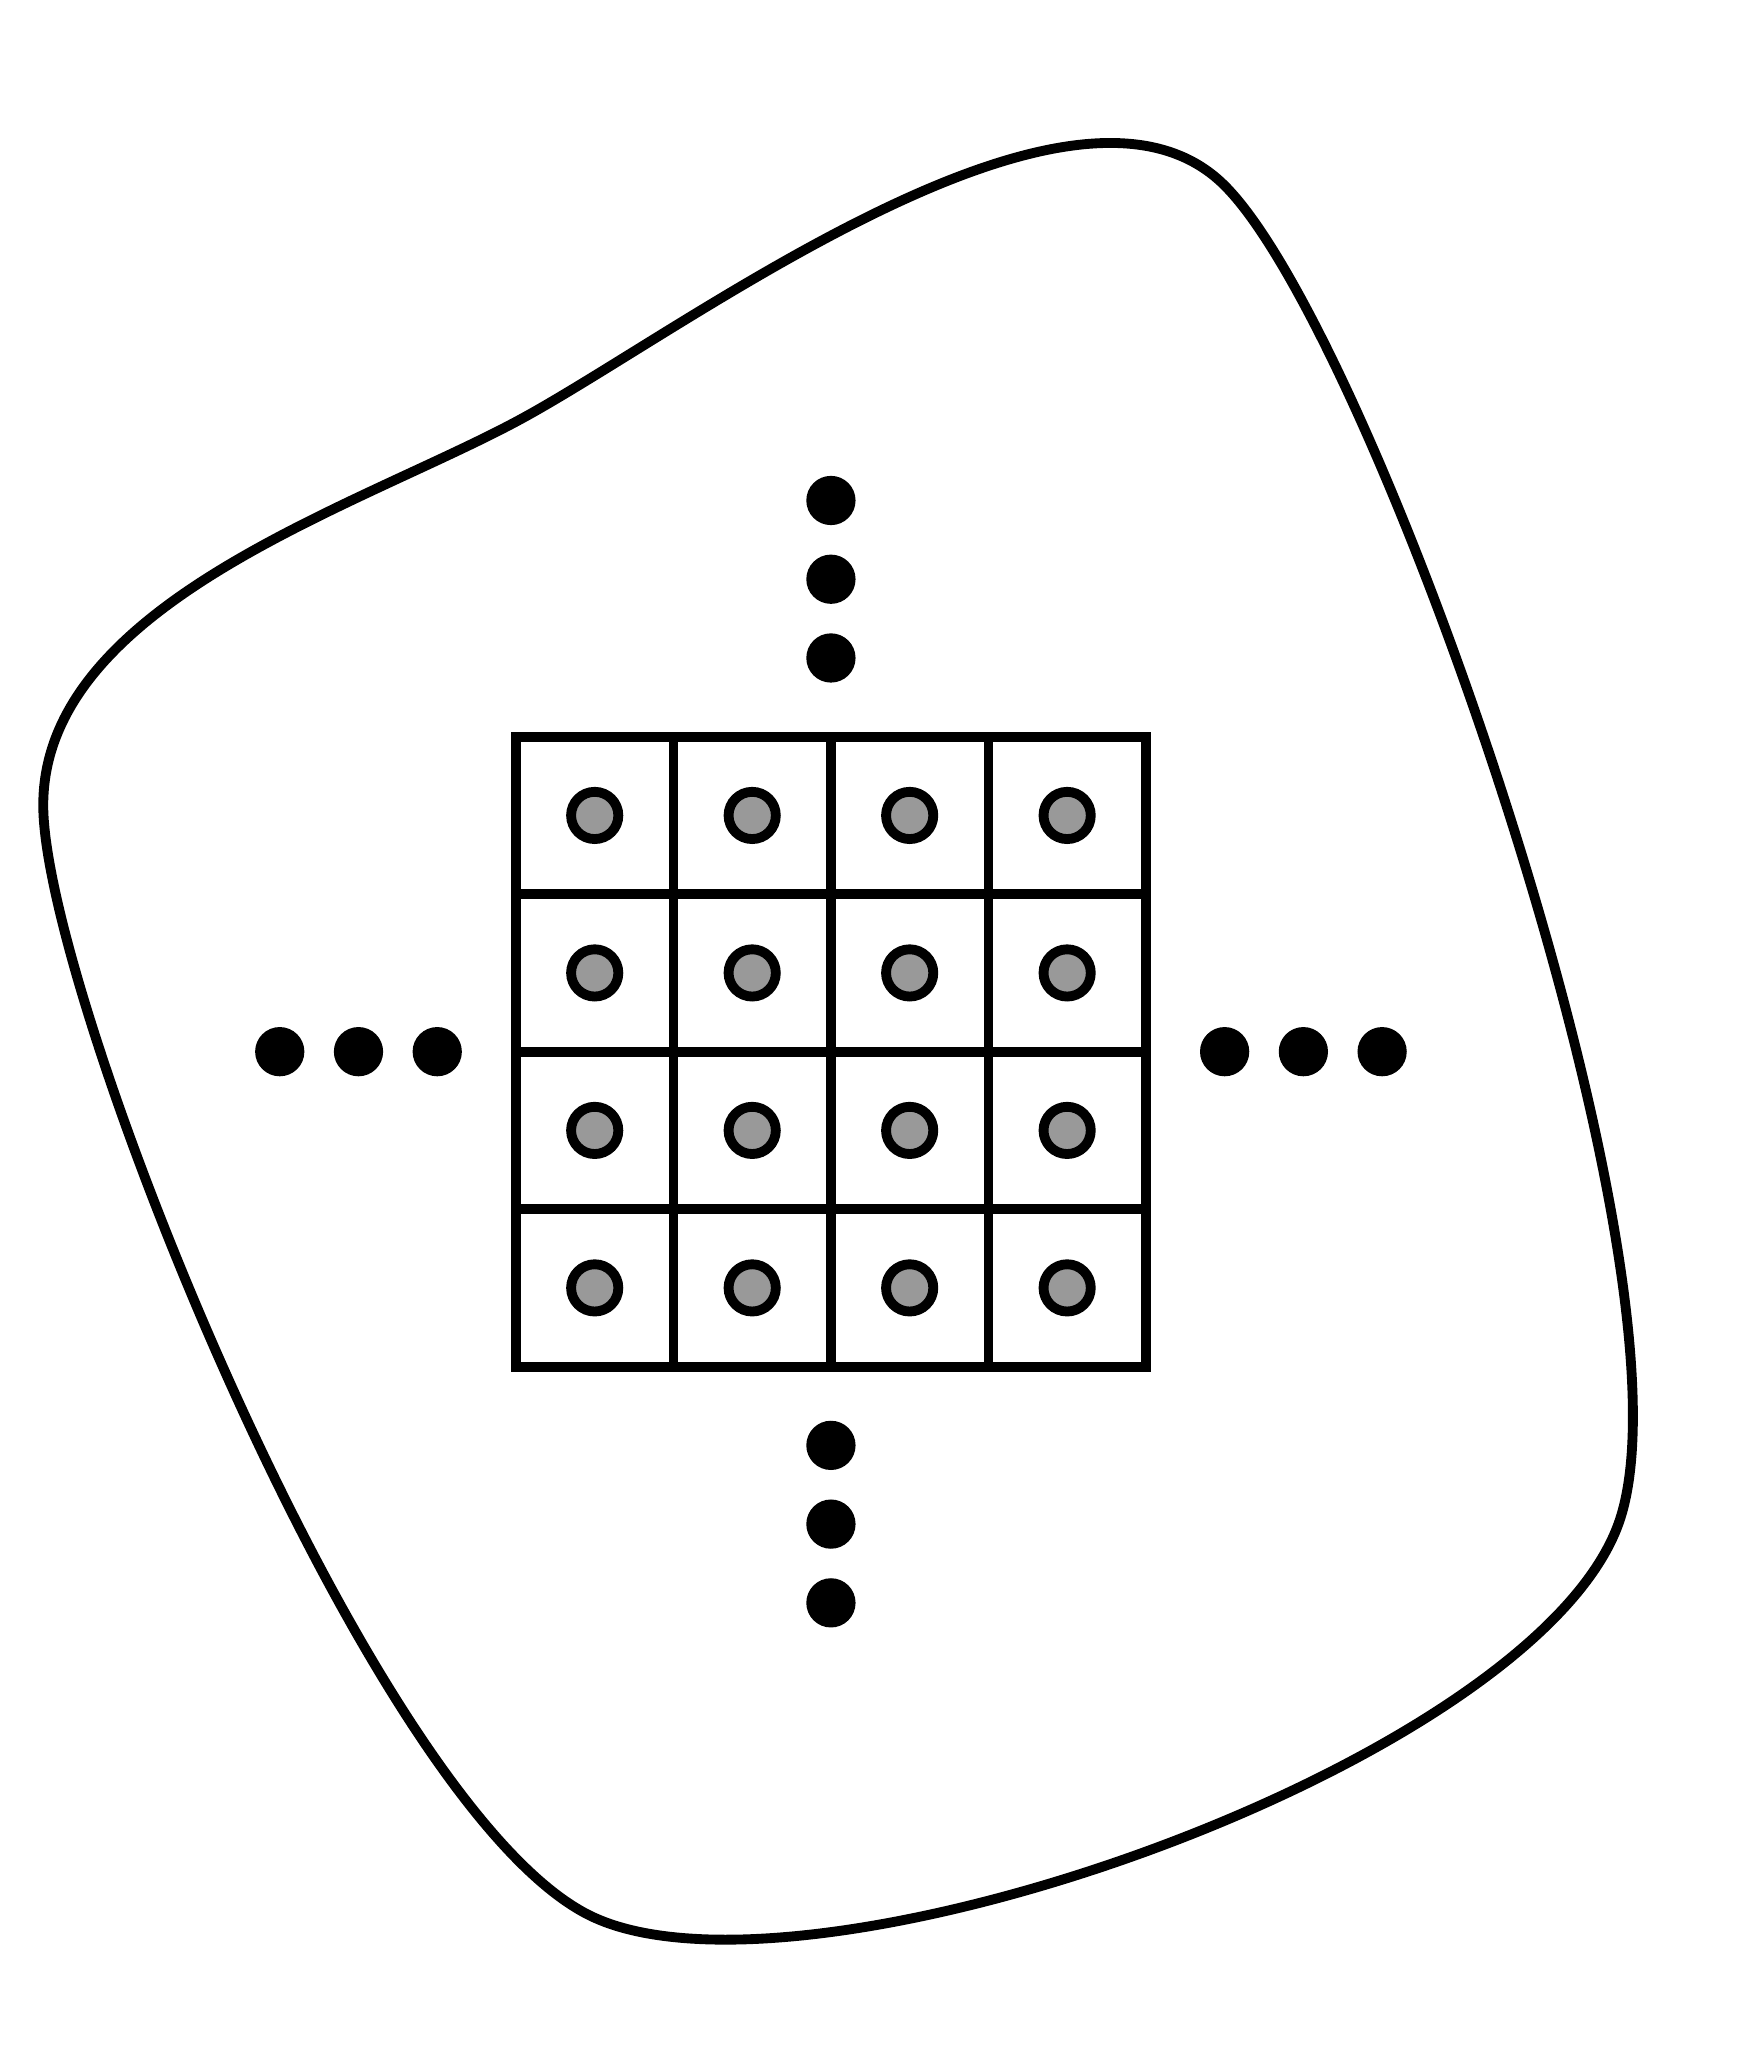
\begin{tikzpicture}[>=latex,node distance=0pt, line width=1.25mm]

    %\draw [gray!50]  (6,15)--(13,1)--(26,6)--(21,23)--(12,20) -- cycle;
    \draw [black] plot [smooth cycle] coordinates {(6,15) (13,1) (26,6) (21,23) (12,20)};

    \begin{scope}[xshift = 4cm]

    \foreach \y [count=\n]in {8,10,12,14}{ 
       \foreach \x [count=\n]in {8,10,12,14}{ 
         \begin{scope}[yshift = \y cm,xshift = \x cm,start chain=going right]
           \draw (0,0) -- (2,0) -- (2,2) -- (0,2) -- cycle;
           \filldraw[fill=black!40!white,draw=black] (1,1) circle (0.3cm);
         \end{scope}
       }
    }

    \filldraw[fill=black,draw=black] (5,12) circle (0.25cm);
    \filldraw[fill=black,draw=black] (6,12) circle (0.25cm);
    \filldraw[fill=black,draw=black] (7,12) circle (0.25cm);

    \filldraw[fill=black,draw=black] (17,12) circle (0.25cm);
    \filldraw[fill=black,draw=black] (18,12) circle (0.25cm);
    \filldraw[fill=black,draw=black] (19,12) circle (0.25cm);

    \filldraw[fill=black,draw=black] (12,5) circle (0.25cm);
    \filldraw[fill=black,draw=black] (12,6) circle (0.25cm);
    \filldraw[fill=black,draw=black] (12,7) circle (0.25cm);

    \filldraw[fill=black,draw=black] (12,17) circle (0.25cm);
    \filldraw[fill=black,draw=black] (12,18) circle (0.25cm);
    \filldraw[fill=black,draw=black] (12,19) circle (0.25cm);

    \end{scope}

\end{tikzpicture}

\end{document}
}
\end{figure}
\end{frame}

%------------------------------------------------

\begin{frame}
\frametitle{FEM directly strategy}
\begin{figure}[!ht]
\resizebox{1.0\linewidth}{!}{\documentclass{standalone}

\begin{document}

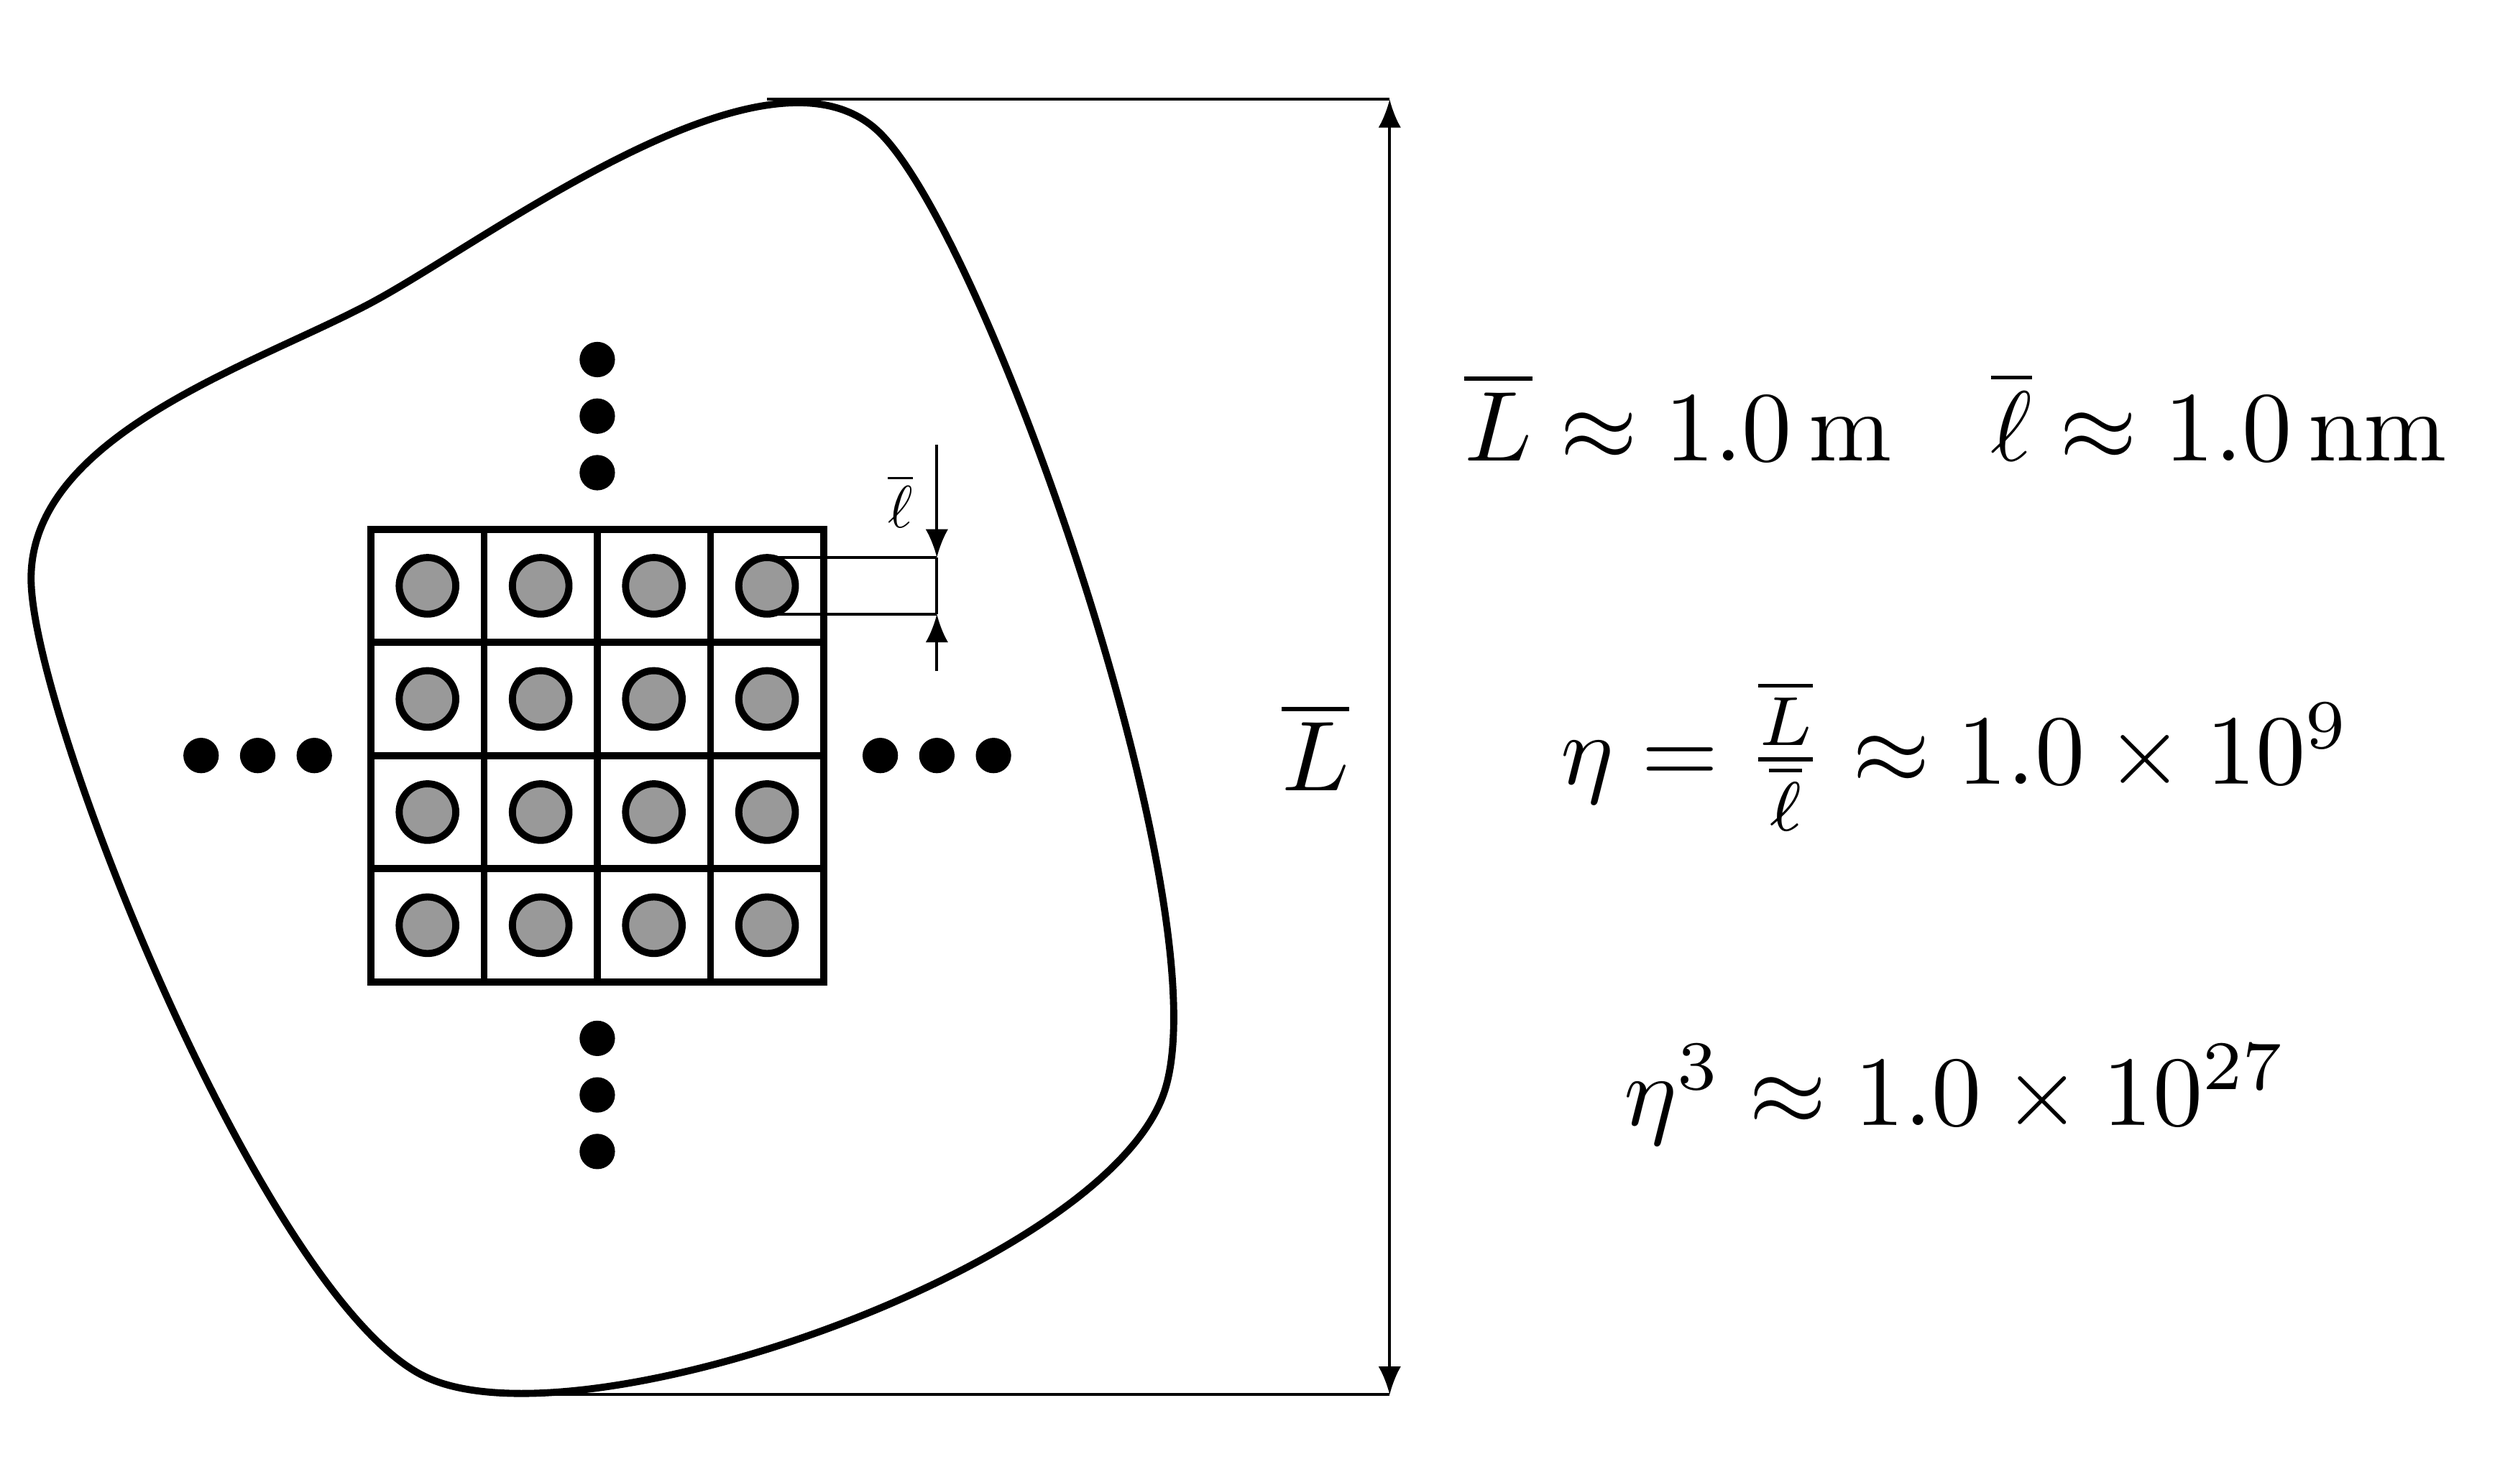
\begin{tikzpicture}[>=latex,node distance=0pt, line width=1.25mm]

    %\draw [gray!50]  (6,15)--(13,1)--(26,6)--(21,23)--(12,20) -- cycle;
    \draw [black] plot [smooth cycle] coordinates {(6,15) (13,1) (26,6) (21,23) (12,20)};

    \begin{scope}[xshift = 4 cm]

    \foreach \y [count=\n]in {8,10,12,14}{ 
       \foreach \x [count=\n]in {8,10,12,14}{ 
         \begin{scope}[yshift = \y cm,xshift = \x cm,start chain=going right]
           \draw (0,0) -- (2,0) -- (2,2) -- (0,2) -- cycle;
           \filldraw[fill=black!40!white,draw=black] (1,1) circle (0.5cm);
         \end{scope}
       }
    }

  \draw[line width=0.5mm] (15,15.5) -- ++(3,0);
  \draw[line width=0.5mm] (15,14.5) -- ++(3,0);
  \draw[line width=0.5mm] (18,14.5) -- ++(0,1);
  \draw[{Latex[length=5mm,width=4mm]}-,line width=0.5mm] (18,14.5) -- ++(0,-1);
  \draw[{Latex[length=5mm,width=4mm]}-,line width=0.5mm] (18,15.5) --
  node[left,rotate=0,scale=3] {$\overline{\ell}$}  ++(0,2);

  %\draw[{Latex[length=5mm,width=4mm]}-{Latex[length=5mm,width=4mm]},line width=0.5mm] 
  %(30,0.7) --  node[left,rotate=0,scale=1] {$\overline{L}$} ++(0,22.9);

  \filldraw[fill=black,draw=black] (5,12) circle (0.25cm);
  \filldraw[fill=black,draw=black] (6,12) circle (0.25cm);
  \filldraw[fill=black,draw=black] (7,12) circle (0.25cm);

  \filldraw[fill=black,draw=black] (17,12) circle (0.25cm);
  \filldraw[fill=black,draw=black] (18,12) circle (0.25cm);
  \filldraw[fill=black,draw=black] (19,12) circle (0.25cm);

  \filldraw[fill=black,draw=black] (12,5) circle (0.25cm);
  \filldraw[fill=black,draw=black] (12,6) circle (0.25cm);
  \filldraw[fill=black,draw=black] (12,7) circle (0.25cm);

  \filldraw[fill=black,draw=black] (12,17) circle (0.25cm);
  \filldraw[fill=black,draw=black] (12,18) circle (0.25cm);
  \filldraw[fill=black,draw=black] (12,19) circle (0.25cm);

  \end{scope}

  \draw[line width=0.5mm] (19,23.6) -- ++(11,0);
  \draw[line width=0.5mm] (15,0.7) -- ++(15,0);
  \draw[{Latex[length=5mm,width=4mm]}-{Latex[length=5mm,width=4mm]},line width=0.5mm] 
  (30,0.7) --  node[left,rotate=0,scale=5] {$\overline{L}$} ++(0,22.9);


  \node[draw=none,fill=none,scale=5] at (40,18) {$\overline{L}\approx\SI{1.0}{\meter} \quad
  \overline{\ell}\approx\SI{1.0}{\nano\meter}$};
  \node[draw=none,fill=none,scale=5] at (40,12) {$\eta = \frac{\overline{L}}{\overline{\ell}} \approx \SI{1.0e9}{}$};
  \node[draw=none,fill=none,scale=5] at (40,6) {$\eta^3 \approx \SI{1.0e27}{}$};

\end{tikzpicture}

\end{document}

}
\end{figure}
\end{frame}

%------------------------------------------------

\begin{frame}
\frametitle{Multi-scale methods}
\begin{figure}[!ht]
\resizebox{1.0\linewidth}{!}{\documentclass{standalone}

\begin{document}

\tikzset{cross/.style={cross out, draw=black, fill=none, minimum size=2*(#1-\pgflinewidth), inner sep=0pt, outer
sep=0pt}, cross/.default={2pt}}

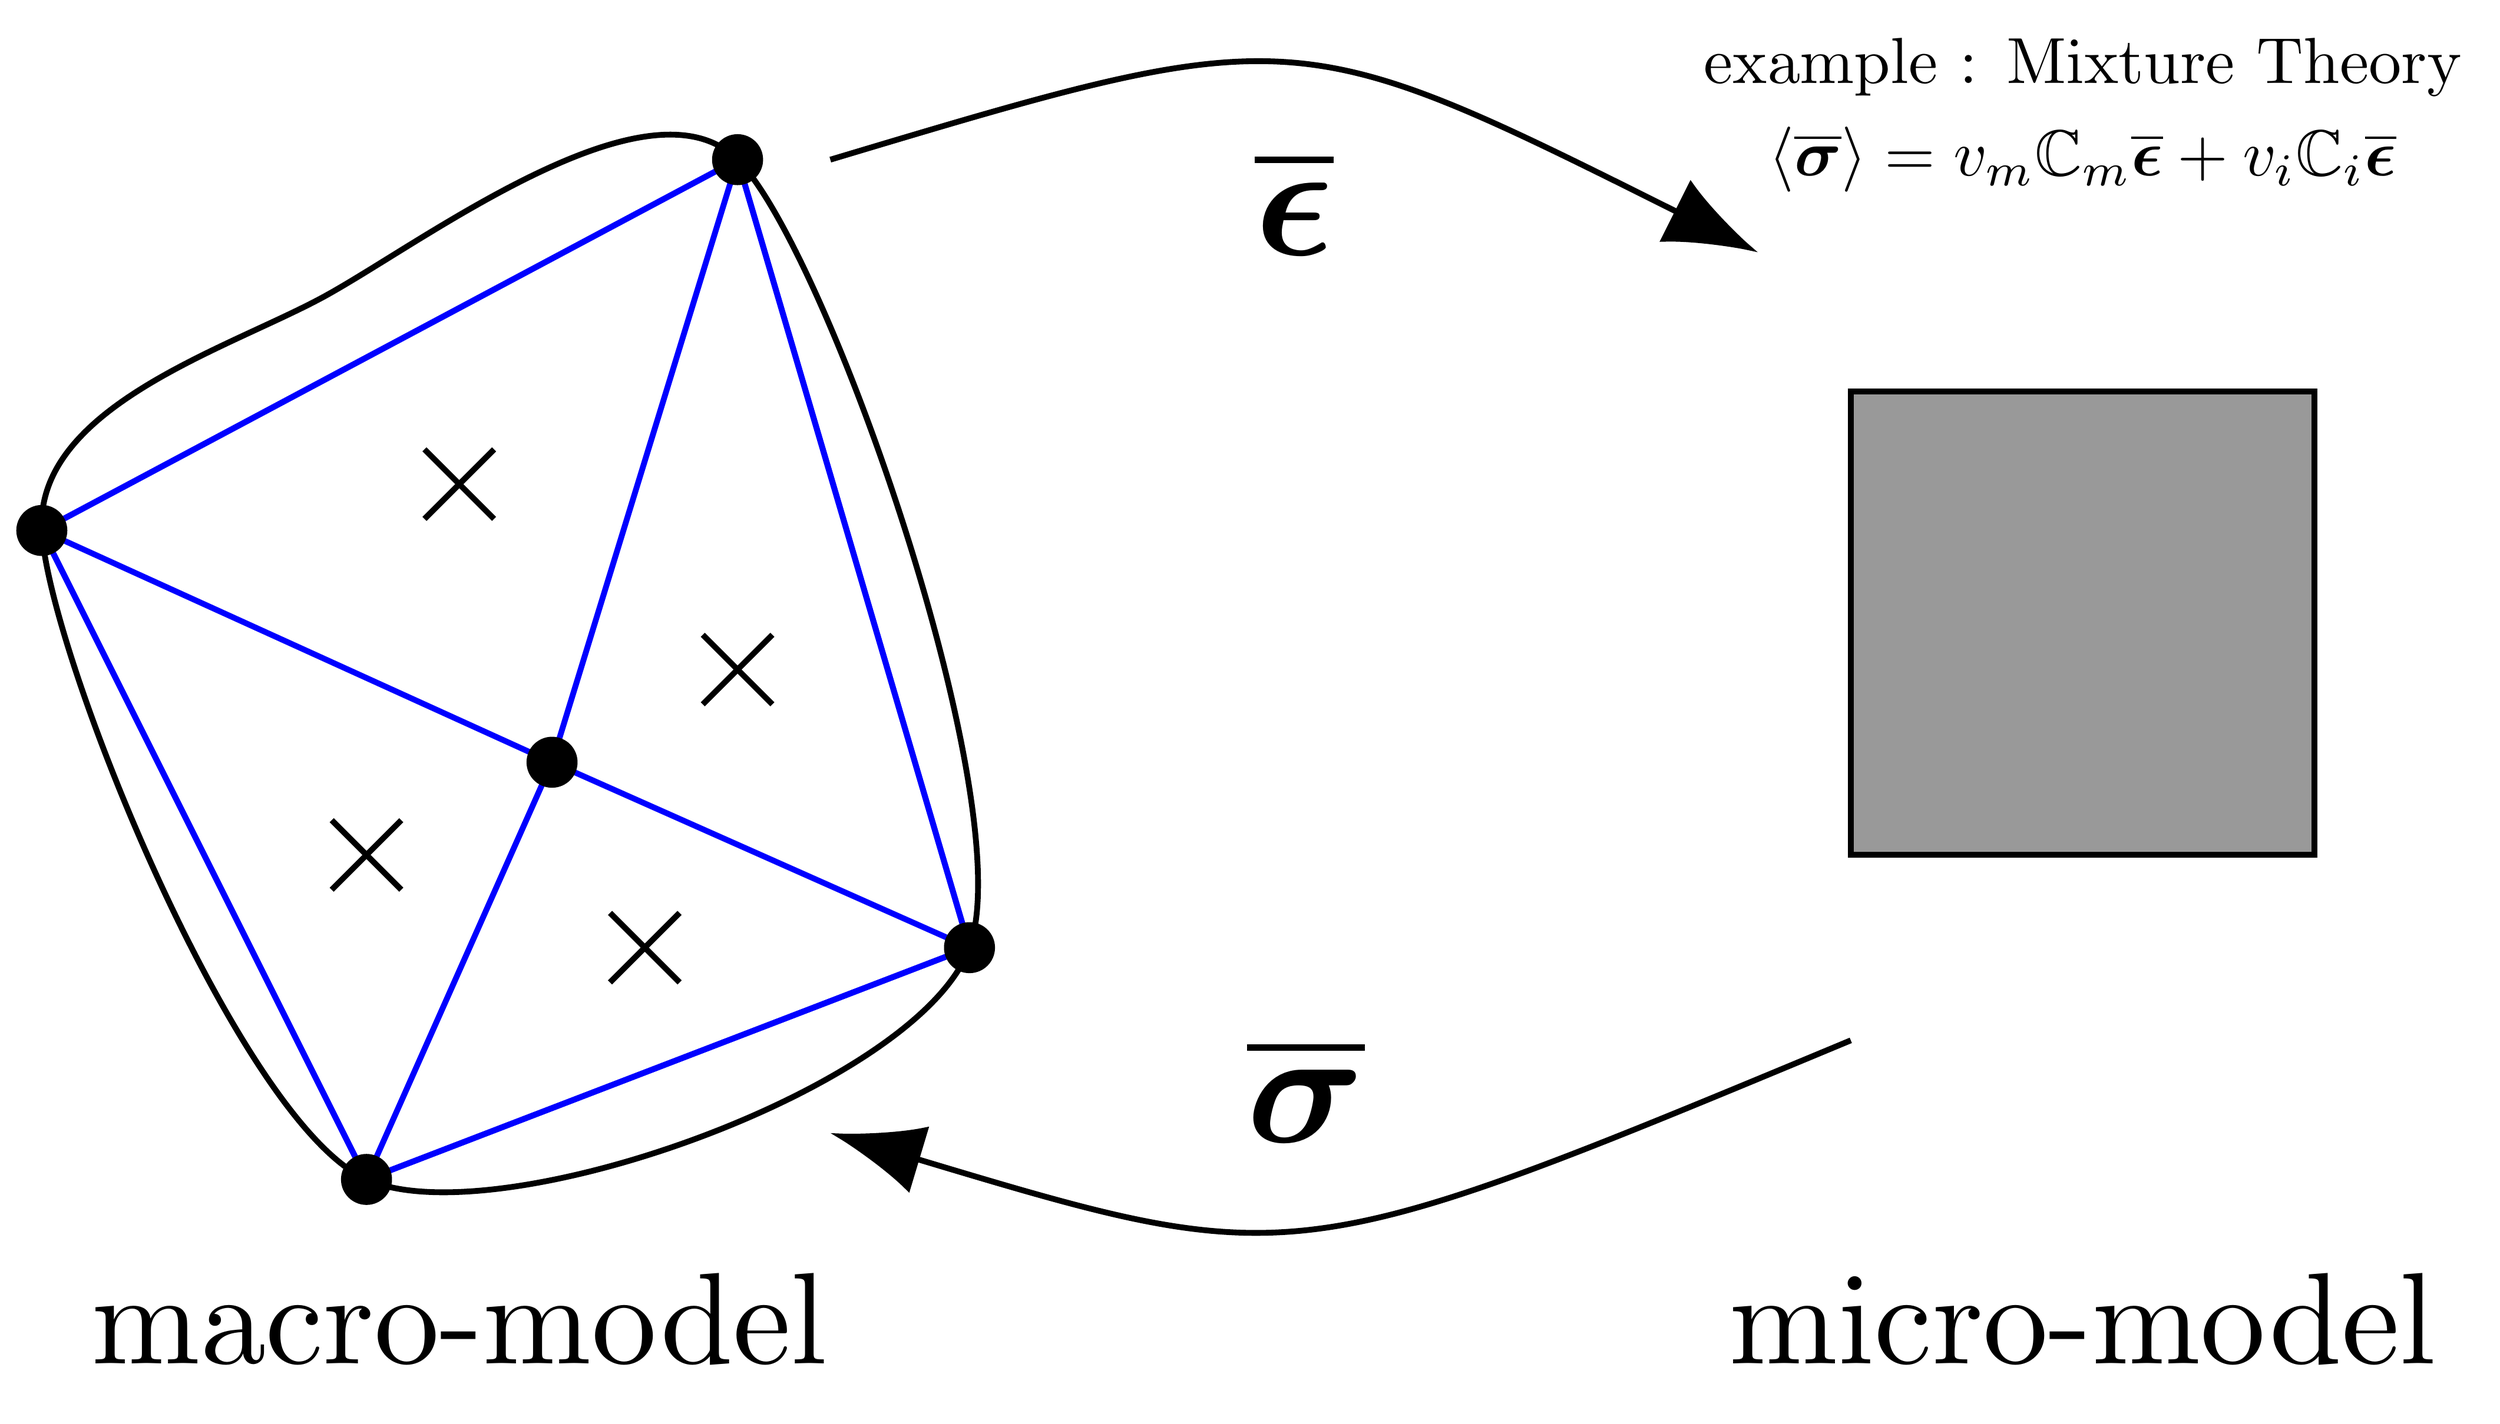
\begin{tikzpicture}[>=latex,node distance=0pt, line width=1.25mm]

% the h.m.s.

    \coordinate [draw=black,shift={(0,0)}] (0) at (6,15);
    \coordinate [draw=black,shift={(0,0)}] (1) at (13,1);
    \coordinate [draw=black,shift={(0,0)}] (2) at (26,6);
    \coordinate [draw=black,shift={(0,0)}] (3) at (21,23);
    \coordinate [draw=black,shift={(0,0)}] (4) at (17,10);
    \draw [blue]  (0) -- (1) -- (2) -- (3) -- cycle;
    \draw [blue]  (0) -- (4);
    \draw [blue]  (1) -- (4);
    \draw [blue]  (2) -- (4);
    \draw [blue]  (3) -- (4);
    \draw [blue]  (6,15) -- (13,1) -- (26,6) -- (21,23) -- cycle;
    \draw [black] plot [smooth cycle] coordinates {(6,15) (13,1) (26,6) (21,23)
    (12,20)};
    \node [fill=black, draw=none, circle, inner sep=0pt, minimum size=1.1cm,scale=1.0] at (0) {};
    \node [fill=black, draw=none, circle, inner sep=0pt, minimum size=1.1cm,scale=1.0] at (1) {};
    \node [fill=black, draw=none, circle, inner sep=0pt, minimum size=1.1cm,scale=1.0] at (2) {};
    \node [fill=black, draw=none, circle, inner sep=0pt, minimum size=1.1cm,scale=1.0] at (3) {};
    \node [fill=black, draw=none, circle, inner sep=0pt, minimum size=1.1cm,scale=1.0] at (4) {};
    \node[cross,minimum size=1.0cm,scale=1.5] (gp_0) at (13,8) {};
    \node[cross,minimum size=1.0cm,scale=1.5] (gp_0) at (15,16) {};
    \node[cross,minimum size=1.0cm,scale=1.5] (gp_0) at (19,6) {};
    \node[cross,minimum size=1.0cm,scale=1.5] (gp_0) at (21,12) {};

% the r.v.e.

    \begin{scope}[yshift = 8 cm,xshift = 45 cm,start chain=going right,scale=5]
          \filldraw[fill=black!40!white,draw=black] (0,0) -- (2,0) -- (2,2) -- (0,2) -- cycle;
    \end{scope}

    \draw[-{Latex[length=20mm,width=15mm]}] (23,23) ..  controls ++(10,+3) ..
    node[below, scale=10] {$\overline{\bm{\epsilon}}$} 
    ++(20,-2);
    \draw[{Latex[length=20mm,width=15mm]}-] (23,2) .. controls ++(10,-3) .. 
    node[above, scale=10] {$\overline{\bm{\sigma}}$}
    ++(22,+2);

    \node[scale=8] at (15,-2) {macro-model} ;
    \node[scale=8] at (50,-2) {micro-model};
    \node[scale=4] at (50,25) {example : Mixture Theory};
    \node[scale=4] at (50,23) {$\langle\overline{\bm{\sigma}}\rangle 
    = v_m \mathbb{C}_m\overline{\bm{\epsilon}} + v_i \mathbb{C}_i\overline{\bm{\epsilon}}$};


\end{tikzpicture}

\end{document}

}
\end{figure}
\end{frame}

%------------------------------------------------

\begin{frame}
\frametitle{The FE$^2$ multi-scale method}
\begin{figure}[!ht]
\resizebox{1.0\linewidth}{!}{\documentclass{standalone}

\begin{document}

\tikzset{cross/.style={cross out, draw=black, fill=none, minimum size=2*(#1-\pgflinewidth), inner sep=0pt, outer
sep=0pt}, cross/.default={2pt}}

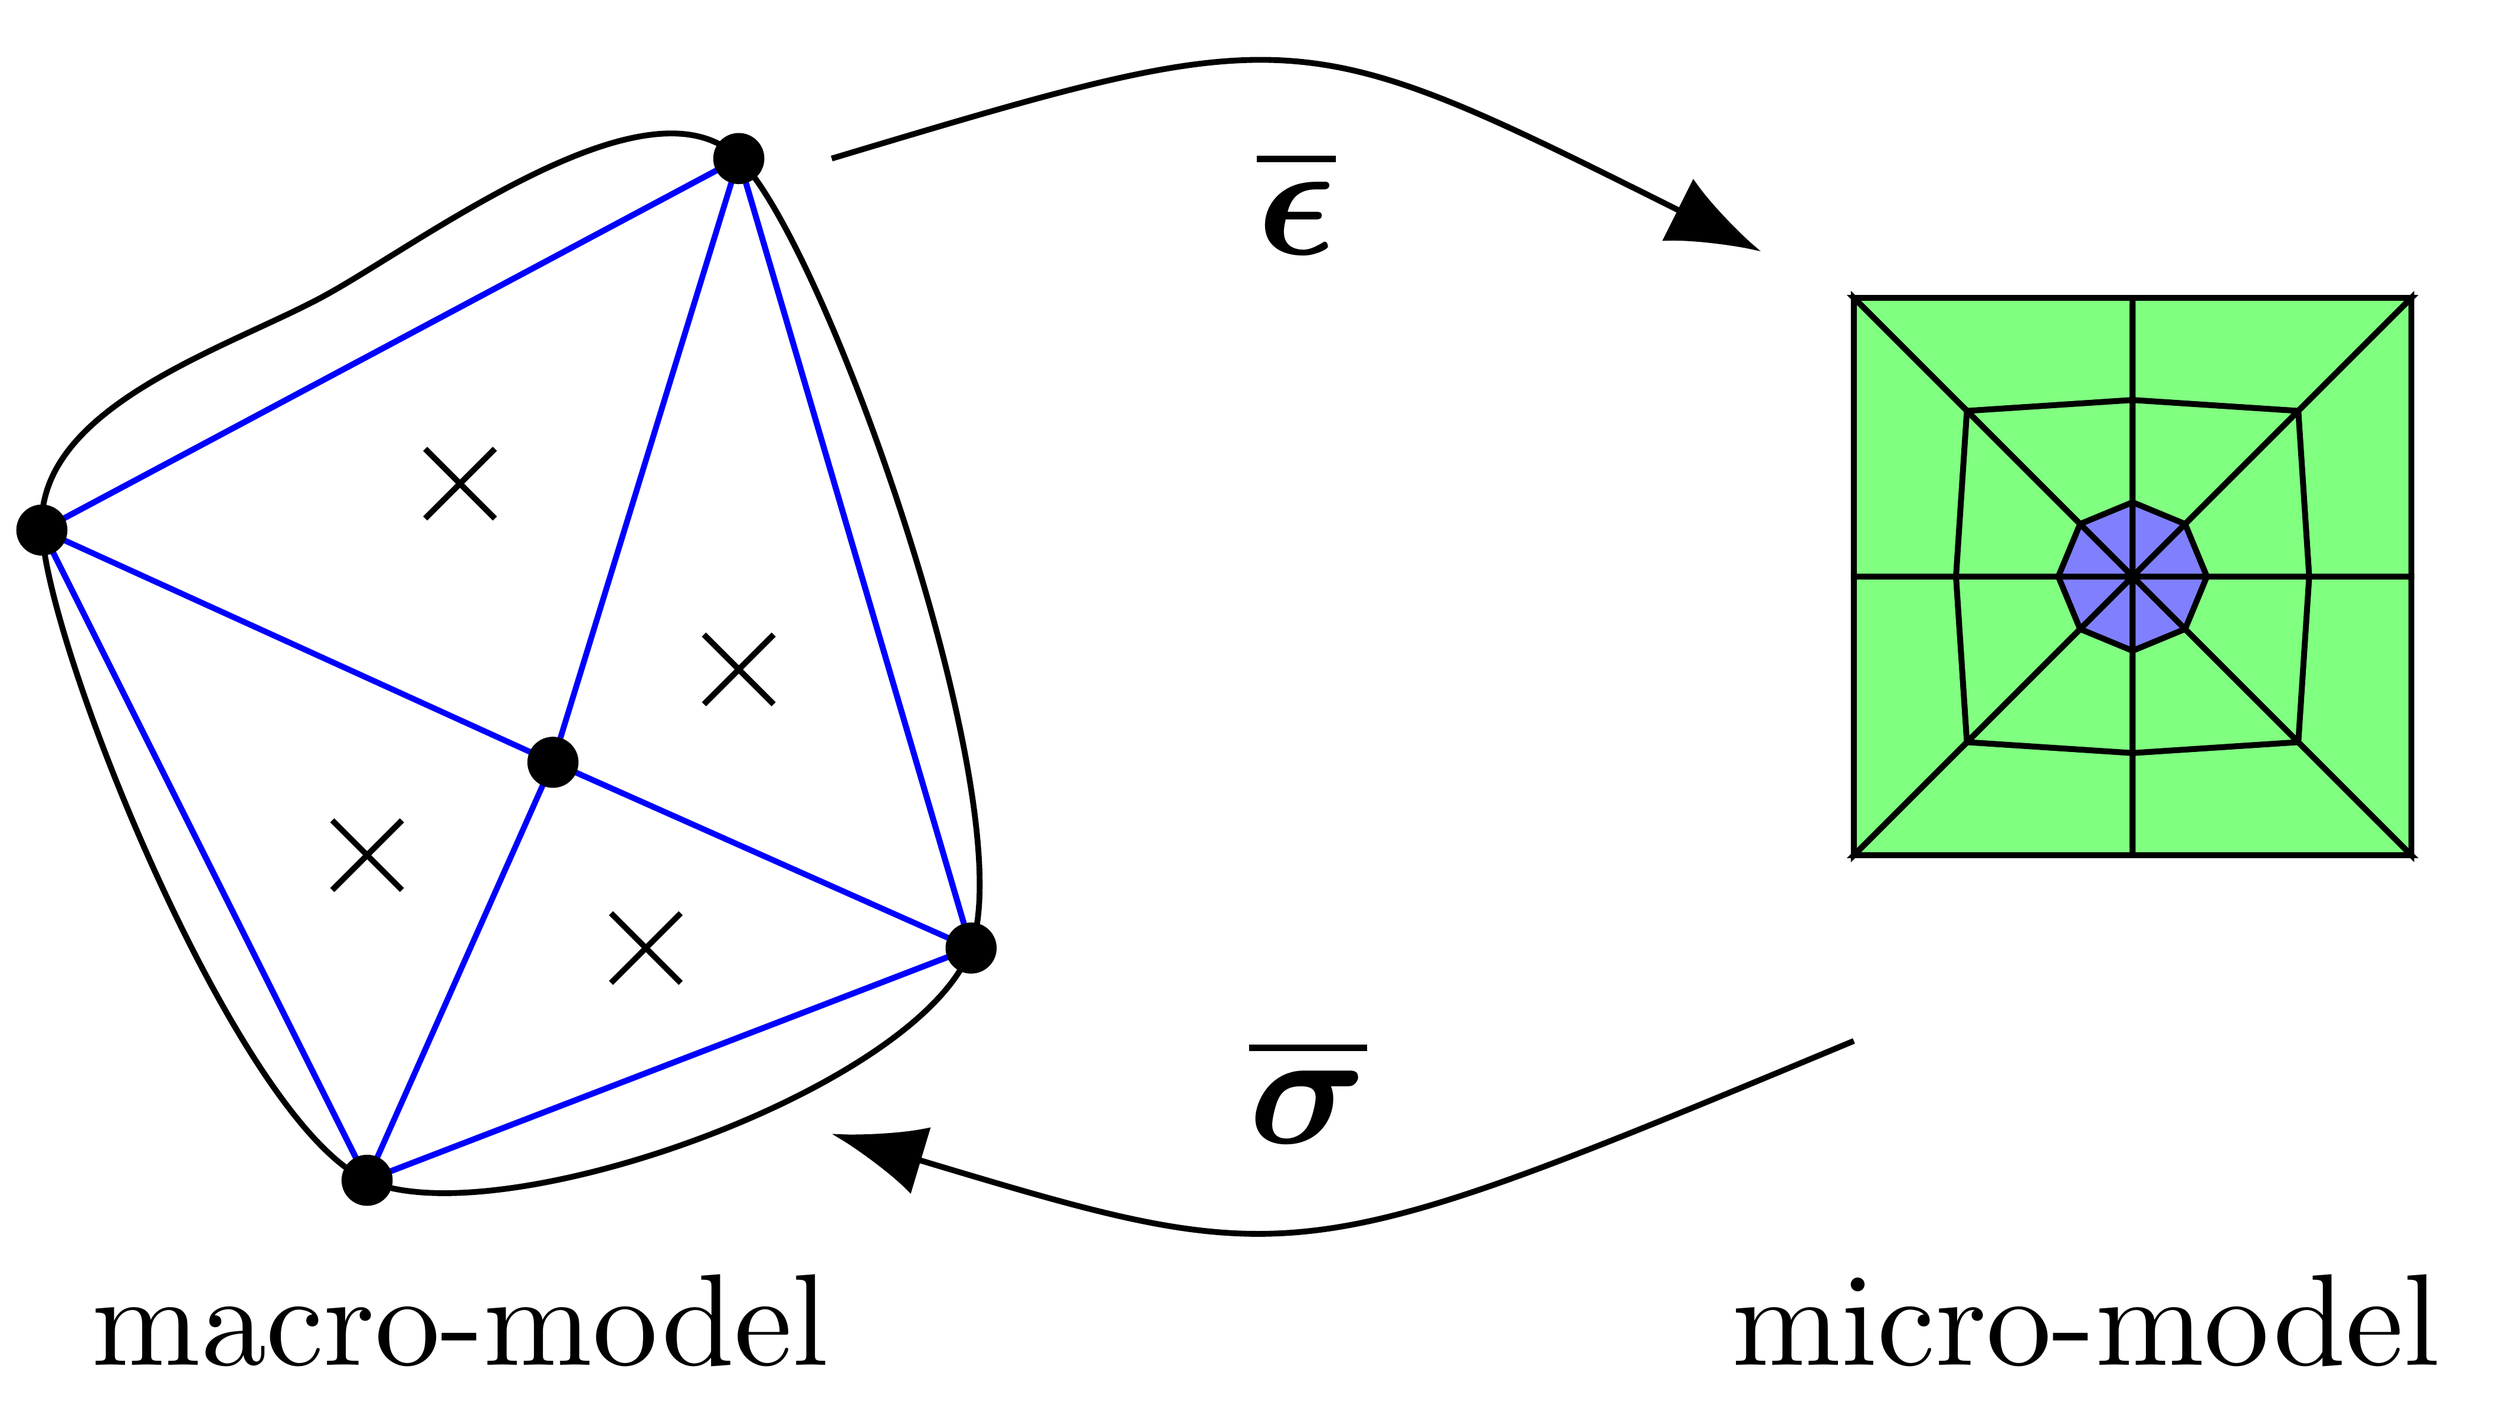
\begin{tikzpicture}[>=latex,node distance=0pt, line width=1.25mm]

% the h.m.s.

    \coordinate [draw=black,shift={(0,0)}] (0) at (6,15);
    \coordinate [draw=black,shift={(0,0)}] (1) at (13,1);
    \coordinate [draw=black,shift={(0,0)}] (2) at (26,6);
    \coordinate [draw=black,shift={(0,0)}] (3) at (21,23);
    \coordinate [draw=black,shift={(0,0)}] (4) at (17,10);
    \draw [blue]  (0) -- (1) -- (2) -- (3) -- cycle;
    \draw [blue]  (0) -- (4);
    \draw [blue]  (1) -- (4);
    \draw [blue]  (2) -- (4);
    \draw [blue]  (3) -- (4);
    \draw [blue]  (6,15) -- (13,1) -- (26,6) -- (21,23) -- cycle;
    \draw [black] plot [smooth cycle] coordinates {(6,15) (13,1) (26,6) (21,23)
    (12,20)};
    \node [fill=black, draw=none, circle, inner sep=0pt, minimum size=1.1cm,scale=1.0] at (0) {};
    \node [fill=black, draw=none, circle, inner sep=0pt, minimum size=1.1cm,scale=1.0] at (1) {};
    \node [fill=black, draw=none, circle, inner sep=0pt, minimum size=1.1cm,scale=1.0] at (2) {};
    \node [fill=black, draw=none, circle, inner sep=0pt, minimum size=1.1cm,scale=1.0] at (3) {};
    \node [fill=black, draw=none, circle, inner sep=0pt, minimum size=1.1cm,scale=1.0] at (4) {};
    \node[cross,minimum size=1.0cm,scale=1.5] (gp_0) at (13,8) {};
    \node[cross,minimum size=1.0cm,scale=1.5] (gp_0) at (15,16) {};
    \node[cross,minimum size=1.0cm,scale=1.5] (gp_0) at (19,6) {};
    \node[cross,minimum size=1.0cm,scale=1.5] (gp_0) at (21,12) {};

% the r.v.e.

    \begin{scope}[yshift = 8 cm,xshift = 45 cm,start chain=going right,scale=4.0]
      \coordinate [draw=black,shift={(0,0)}] (0) at (0,0);
      \coordinate [draw=black,shift={(0,0)}] (1) at (1.5,0);
      \coordinate [draw=black,shift={(0,0)}] (2) at (1.5,1.5);
      \coordinate [draw=black,shift={(0,0)}] (3) at (1.5,1.1);
      \coordinate [draw=black,shift={(0,0)}] (4) at (1.2171572876,1.2171572876);
      \coordinate [draw=black,shift={(0,0)}] (5) at (1.1,1.5);
      \coordinate [draw=black,shift={(0,0)}] (6) at (0,1.5);
      \coordinate [draw=black,shift={(0,0)}] (7) at (0,3);
      \coordinate [draw=black,shift={(0,0)}] (8) at (1.2171572876,1.7828427124);
      \coordinate [draw=black,shift={(0,0)}] (9) at (1.5,1.9);
      \coordinate [draw=black,shift={(0,0)}] (10) at (1.5,3);
      \coordinate [draw=black,shift={(0,0)}] (11) at (3,0);
      \coordinate [draw=black,shift={(0,0)}] (12) at (1.7828427124,1.2171572876);
      \coordinate [draw=black,shift={(0,0)}] (13) at (1.9,1.5);
      \coordinate [draw=black,shift={(0,0)}] (14) at (3,1.5);
      \coordinate [draw=black,shift={(0,0)}] (15) at (3,3);
      \coordinate [draw=black,shift={(0,0)}] (16) at (1.7828427124,1.7828427124);
      \coordinate [draw=black,shift={(0,0)}] (17) at (1.5,0.5500000000014312);
      \coordinate [draw=black,shift={(0,0)}] (18) at (0.6085786437983935,0.6085786437983935);
      \coordinate [draw=black,shift={(0,0)}] (19) at (0.5500000000014312,1.5);
      \coordinate [draw=black,shift={(0,0)}] (20) at (0.6085786437983723,2.391421356201628);
      \coordinate [draw=black,shift={(0,0)}] (21) at (1.5,2.449999999998004);
      \coordinate [draw=black,shift={(0,0)}] (22) at (2.391421356201628,0.6085786437983723);
      \coordinate [draw=black,shift={(0,0)}] (23) at (2.449999999998004,1.5);
      \coordinate [draw=black,shift={(0,0)}] (24) at (2.391421356201648,2.391421356201648);
      \draw [fill=blue!50] (2) --  (4) --  (3) -- cycle;
      \draw [fill=blue!50] (2) --  (4) --  (5) -- cycle;
      \draw [fill=blue!50] (2) --  (8) --  (9) -- cycle;
      \draw [fill=blue!50] (2) --  (8) --  (5) -- cycle;
      \draw [fill=blue!50] (2) --  (12) --  (3) -- cycle;
      \draw [fill=blue!50] (2) --  (12) --  (13) -- cycle;
      \draw [fill=blue!50] (2) --  (16) --  (9) -- cycle;
      \draw [fill=blue!50] (2) --  (16) --  (13) -- cycle;
      \draw [fill=green!50] (0) --  (18) --  (17) --  (1) -- cycle;
      \draw [fill=green!50] (18) --  (4) --  (3) --  (17) -- cycle;
      \draw [fill=green!50] (0) --  (18) --  (19) --  (6) -- cycle;
      \draw [fill=green!50] (18) --  (4) --  (5) --  (19) -- cycle;
      \draw [fill=green!50] (7) --  (20) --  (21) --  (10) -- cycle;
      \draw [fill=green!50] (20) --  (8) --  (9) --  (21) -- cycle;
      \draw [fill=green!50] (7) --  (20) --  (19) --  (6) -- cycle;
      \draw [fill=green!50] (20) --  (8) --  (5) --  (19) -- cycle;
      \draw [fill=green!50] (11) --  (22) --  (17) --  (1) -- cycle;
      \draw [fill=green!50] (22) --  (12) --  (3) --  (17) -- cycle;
      \draw [fill=green!50] (11) --  (22) --  (23) --  (14) -- cycle;
      \draw [fill=green!50] (22) --  (12) --  (13) --  (23) -- cycle;
      \draw [fill=green!50] (15) --  (24) --  (21) --  (10) -- cycle;
      \draw [fill=green!50] (24) --  (16) --  (9) --  (21) -- cycle;
      \draw [fill=green!50] (15) --  (24) --  (23) --  (14) -- cycle;
      \draw [fill=green!50] (24) --  (16) --  (13) --  (23) -- cycle;
      \node [fill=black, draw=none, circle, inner sep=0pt, minimum size=0.1cm,scale=0.3] at (0) {h};
      \node [fill=black, draw=none, circle, inner sep=0pt, minimum size=0.1cm,scale=0.3] at (1) {h};
      \node [fill=black, draw=none, circle, inner sep=0pt, minimum size=0.1cm,scale=0.3] at (2) {h};
      \node [fill=black, draw=none, circle, inner sep=0pt, minimum size=0.1cm,scale=0.3] at (3) {h};
      \node [fill=black, draw=none, circle, inner sep=0pt, minimum size=0.1cm,scale=0.3] at (4) {h};
      \node [fill=black, draw=none, circle, inner sep=0pt, minimum size=0.1cm,scale=0.3] at (5) {h};
      \node [fill=black, draw=none, circle, inner sep=0pt, minimum size=0.1cm,scale=0.3] at (6) {h};
      \node [fill=black, draw=none, circle, inner sep=0pt, minimum size=0.1cm,scale=0.3] at (7) {h};
      \node [fill=black, draw=none, circle, inner sep=0pt, minimum size=0.1cm,scale=0.3] at (8) {h};
      \node [fill=black, draw=none, circle, inner sep=0pt, minimum size=0.1cm,scale=0.3] at (9) {h};
      \node [fill=black, draw=none, circle, inner sep=0pt, minimum size=0.1cm,scale=0.3] at (10) {h};
      \node [fill=black, draw=none, circle, inner sep=0pt, minimum size=0.1cm,scale=0.3] at (11) {h};
      \node [fill=black, draw=none, circle, inner sep=0pt, minimum size=0.1cm,scale=0.3] at (12) {h};
      \node [fill=black, draw=none, circle, inner sep=0pt, minimum size=0.1cm,scale=0.3] at (13) {h};
      \node [fill=black, draw=none, circle, inner sep=0pt, minimum size=0.1cm,scale=0.3] at (14) {h};
      \node [fill=black, draw=none, circle, inner sep=0pt, minimum size=0.1cm,scale=0.3] at (15) {h};
      \node [fill=black, draw=none, circle, inner sep=0pt, minimum size=0.1cm,scale=0.3] at (16) {h};
      \node [fill=black, draw=none, circle, inner sep=0pt, minimum size=0.1cm,scale=0.3] at (17) {h};
      \node [fill=black, draw=none, circle, inner sep=0pt, minimum size=0.1cm,scale=0.3] at (18) {h};
      \node [fill=black, draw=none, circle, inner sep=0pt, minimum size=0.1cm,scale=0.3] at (19) {h};
      \node [fill=black, draw=none, circle, inner sep=0pt, minimum size=0.1cm,scale=0.3] at (20) {h};
      \node [fill=black, draw=none, circle, inner sep=0pt, minimum size=0.1cm,scale=0.3] at (21) {h};
      \node [fill=black, draw=none, circle, inner sep=0pt, minimum size=0.1cm,scale=0.3] at (22) {h};
      \node [fill=black, draw=none, circle, inner sep=0pt, minimum size=0.1cm,scale=0.3] at (23) {h};
      \node [fill=black, draw=none, circle, inner sep=0pt, minimum size=0.1cm,scale=0.3] at (24) {h};
    \end{scope}

    \draw[-{Latex[length=20mm,width=15mm]}] (23,23) ..  controls ++(10,+3) ..
    node[below, scale=10] {$\overline{\bm{\epsilon}}$} 
    ++(20,-2);
    \draw[{Latex[length=20mm,width=15mm]}-] (23,2) .. controls ++(10,-3) .. 
    node[above, scale=10] {$\overline{\bm{\sigma}}$}
    ++(22,+2);

    \node[scale=8] at (15,-2) {macro-model} ;
    \node[scale=8] at (50,-2) {micro-model};

\end{tikzpicture}

\end{document}

}
\end{figure}
\end{frame}

%------------------------------------------------

\begin{frame}
\frametitle{The micro-problem in the FE$^2$ method}
\begin{figure}[!ht]
\resizebox{0.8\linewidth}{!}{\documentclass{standalone}

\begin{document}

\tikzset{cross/.style={cross out, draw=black, fill=none, minimum size=2*(#1-\pgflinewidth), inner sep=0pt, outer
sep=0pt}, cross/.default={2pt}}

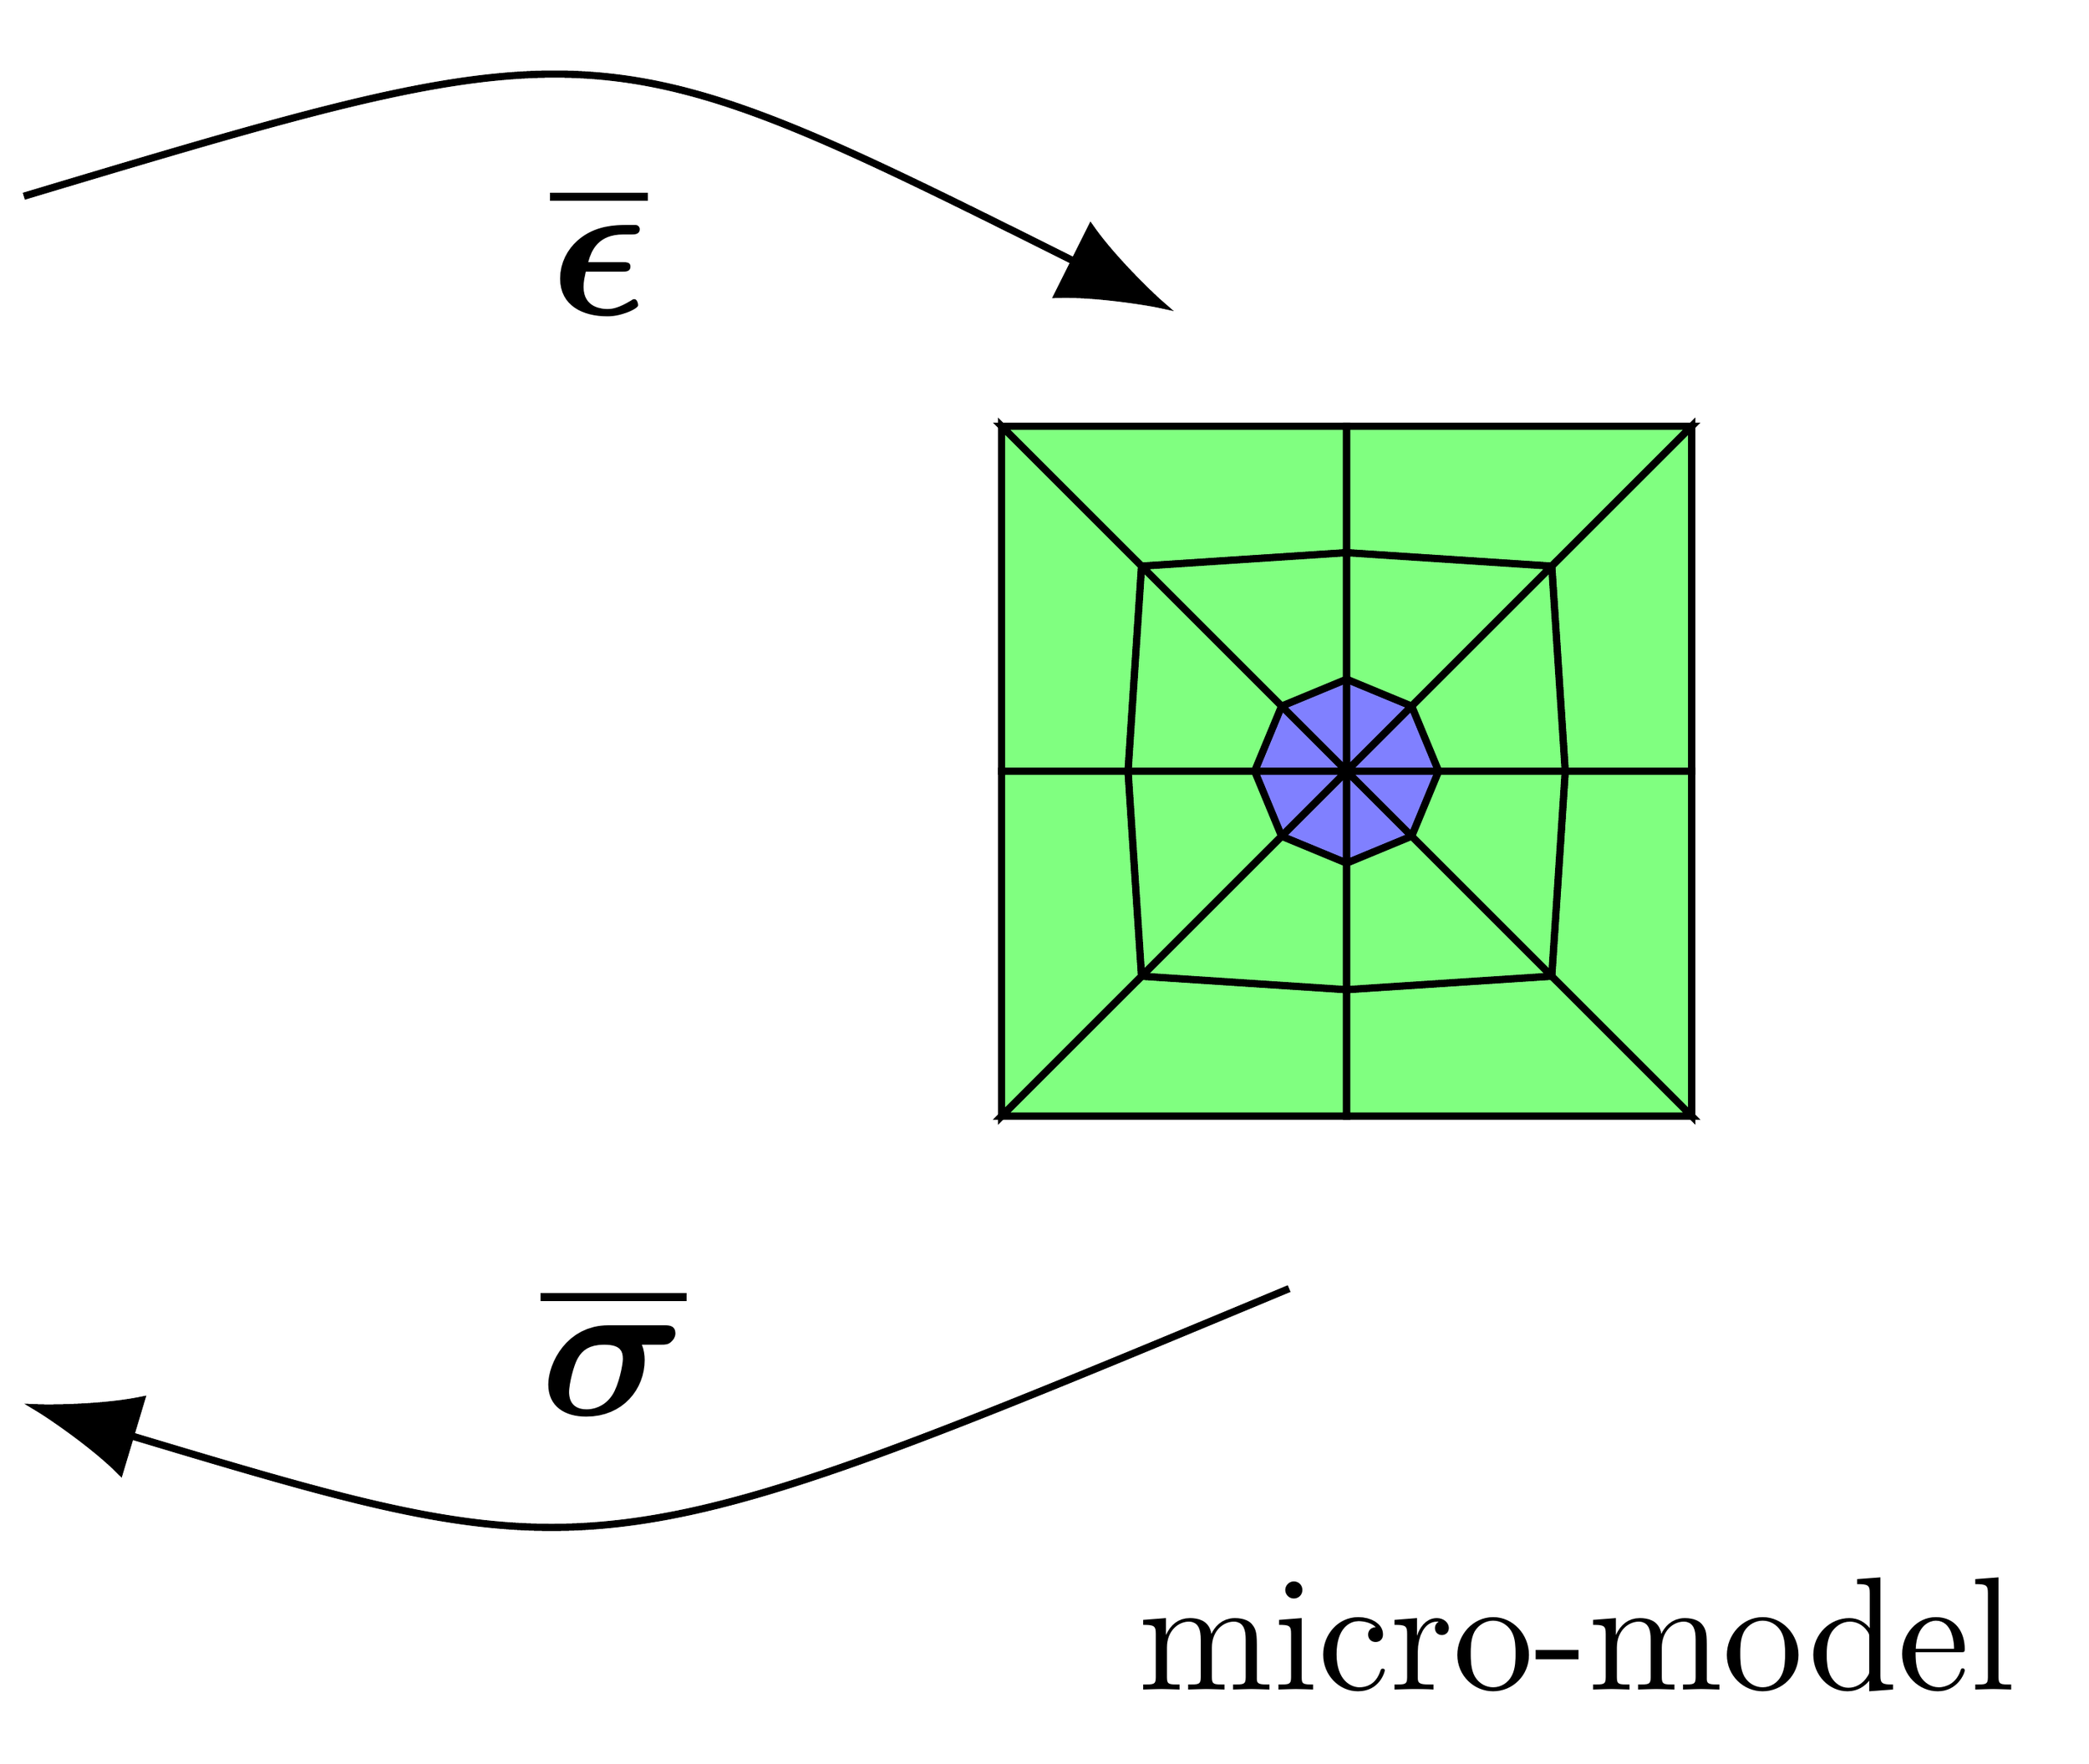
\begin{tikzpicture}[>=latex,node distance=0pt, line width=1.25mm]

    \begin{scope}[yshift=7 cm, xshift=40cm, start chain=going right, scale=4.0]
      \coordinate [draw=black,shift={(0,0)}] (0) at (0,0);
      \coordinate [draw=black,shift={(0,0)}] (1) at (1.5,0);
      \coordinate [draw=black,shift={(0,0)}] (2) at (1.5,1.5);
      \coordinate [draw=black,shift={(0,0)}] (3) at (1.5,1.1);
      \coordinate [draw=black,shift={(0,0)}] (4) at (1.2171572876,1.2171572876);
      \coordinate [draw=black,shift={(0,0)}] (5) at (1.1,1.5);
      \coordinate [draw=black,shift={(0,0)}] (6) at (0,1.5);
      \coordinate [draw=black,shift={(0,0)}] (7) at (0,3);
      \coordinate [draw=black,shift={(0,0)}] (8) at (1.2171572876,1.7828427124);
      \coordinate [draw=black,shift={(0,0)}] (9) at (1.5,1.9);
      \coordinate [draw=black,shift={(0,0)}] (10) at (1.5,3);
      \coordinate [draw=black,shift={(0,0)}] (11) at (3,0);
      \coordinate [draw=black,shift={(0,0)}] (12) at (1.7828427124,1.2171572876);
      \coordinate [draw=black,shift={(0,0)}] (13) at (1.9,1.5);
      \coordinate [draw=black,shift={(0,0)}] (14) at (3,1.5);
      \coordinate [draw=black,shift={(0,0)}] (15) at (3,3);
      \coordinate [draw=black,shift={(0,0)}] (16) at (1.7828427124,1.7828427124);
      \coordinate [draw=black,shift={(0,0)}] (17) at (1.5,0.5500000000014312);
      \coordinate [draw=black,shift={(0,0)}] (18) at (0.6085786437983935,0.6085786437983935);
      \coordinate [draw=black,shift={(0,0)}] (19) at (0.5500000000014312,1.5);
      \coordinate [draw=black,shift={(0,0)}] (20) at (0.6085786437983723,2.391421356201628);
      \coordinate [draw=black,shift={(0,0)}] (21) at (1.5,2.449999999998004);
      \coordinate [draw=black,shift={(0,0)}] (22) at (2.391421356201628,0.6085786437983723);
      \coordinate [draw=black,shift={(0,0)}] (23) at (2.449999999998004,1.5);
      \coordinate [draw=black,shift={(0,0)}] (24) at (2.391421356201648,2.391421356201648);
      \draw [fill=blue!50] (2) --  (4) --  (3) -- cycle;
      \draw [fill=blue!50] (2) --  (4) --  (5) -- cycle;
      \draw [fill=blue!50] (2) --  (8) --  (9) -- cycle;
      \draw [fill=blue!50] (2) --  (8) --  (5) -- cycle;
      \draw [fill=blue!50] (2) --  (12) --  (3) -- cycle;
      \draw [fill=blue!50] (2) --  (12) --  (13) -- cycle;
      \draw [fill=blue!50] (2) --  (16) --  (9) -- cycle;
      \draw [fill=blue!50] (2) --  (16) --  (13) -- cycle;
      \draw [fill=green!50] (0) --  (18) --  (17) --  (1) -- cycle;
      \draw [fill=green!50] (18) --  (4) --  (3) --  (17) -- cycle;
      \draw [fill=green!50] (0) --  (18) --  (19) --  (6) -- cycle;
      \draw [fill=green!50] (18) --  (4) --  (5) --  (19) -- cycle;
      \draw [fill=green!50] (7) --  (20) --  (21) --  (10) -- cycle;
      \draw [fill=green!50] (20) --  (8) --  (9) --  (21) -- cycle;
      \draw [fill=green!50] (7) --  (20) --  (19) --  (6) -- cycle;
      \draw [fill=green!50] (20) --  (8) --  (5) --  (19) -- cycle;
      \draw [fill=green!50] (11) --  (22) --  (17) --  (1) -- cycle;
      \draw [fill=green!50] (22) --  (12) --  (3) --  (17) -- cycle;
      \draw [fill=green!50] (11) --  (22) --  (23) --  (14) -- cycle;
      \draw [fill=green!50] (22) --  (12) --  (13) --  (23) -- cycle;
      \draw [fill=green!50] (15) --  (24) --  (21) --  (10) -- cycle;
      \draw [fill=green!50] (24) --  (16) --  (9) --  (21) -- cycle;
      \draw [fill=green!50] (15) --  (24) --  (23) --  (14) -- cycle;
      \draw [fill=green!50] (24) --  (16) --  (13) --  (23) -- cycle;
      \node [fill=black, draw=none, circle, inner sep=0pt, minimum size=0.1cm,scale=0.3] at (0) {h};
      \node [fill=black, draw=none, circle, inner sep=0pt, minimum size=0.1cm,scale=0.3] at (1) {h};
      \node [fill=black, draw=none, circle, inner sep=0pt, minimum size=0.1cm,scale=0.3] at (2) {h};
      \node [fill=black, draw=none, circle, inner sep=0pt, minimum size=0.1cm,scale=0.3] at (3) {h};
      \node [fill=black, draw=none, circle, inner sep=0pt, minimum size=0.1cm,scale=0.3] at (4) {h};
      \node [fill=black, draw=none, circle, inner sep=0pt, minimum size=0.1cm,scale=0.3] at (5) {h};
      \node [fill=black, draw=none, circle, inner sep=0pt, minimum size=0.1cm,scale=0.3] at (6) {h};
      \node [fill=black, draw=none, circle, inner sep=0pt, minimum size=0.1cm,scale=0.3] at (7) {h};
      \node [fill=black, draw=none, circle, inner sep=0pt, minimum size=0.1cm,scale=0.3] at (8) {h};
      \node [fill=black, draw=none, circle, inner sep=0pt, minimum size=0.1cm,scale=0.3] at (9) {h};
      \node [fill=black, draw=none, circle, inner sep=0pt, minimum size=0.1cm,scale=0.3] at (10) {h};
      \node [fill=black, draw=none, circle, inner sep=0pt, minimum size=0.1cm,scale=0.3] at (11) {h};
      \node [fill=black, draw=none, circle, inner sep=0pt, minimum size=0.1cm,scale=0.3] at (12) {h};
      \node [fill=black, draw=none, circle, inner sep=0pt, minimum size=0.1cm,scale=0.3] at (13) {h};
      \node [fill=black, draw=none, circle, inner sep=0pt, minimum size=0.1cm,scale=0.3] at (14) {h};
      \node [fill=black, draw=none, circle, inner sep=0pt, minimum size=0.1cm,scale=0.3] at (15) {h};
      \node [fill=black, draw=none, circle, inner sep=0pt, minimum size=0.1cm,scale=0.3] at (16) {h};
      \node [fill=black, draw=none, circle, inner sep=0pt, minimum size=0.1cm,scale=0.3] at (17) {h};
      \node [fill=black, draw=none, circle, inner sep=0pt, minimum size=0.1cm,scale=0.3] at (18) {h};
      \node [fill=black, draw=none, circle, inner sep=0pt, minimum size=0.1cm,scale=0.3] at (19) {h};
      \node [fill=black, draw=none, circle, inner sep=0pt, minimum size=0.1cm,scale=0.3] at (20) {h};
      \node [fill=black, draw=none, circle, inner sep=0pt, minimum size=0.1cm,scale=0.3] at (21) {h};
      \node [fill=black, draw=none, circle, inner sep=0pt, minimum size=0.1cm,scale=0.3] at (22) {h};
      \node [fill=black, draw=none, circle, inner sep=0pt, minimum size=0.1cm,scale=0.3] at (23) {h};
      \node [fill=black, draw=none, circle, inner sep=0pt, minimum size=0.1cm,scale=0.3] at (24) {h};
    \end{scope}

    \draw[-{Latex[length=20mm,width=15mm]}] (23,23) ..  controls ++(10,+3) ..
    node[below, scale=10] {$\overline{\bm{\epsilon}}$} 
    ++(20,-2);
    \draw[{Latex[length=20mm,width=15mm]}-] (23,2) .. controls ++(10,-3) .. 
    node[above, scale=10] {$\overline{\bm{\sigma}}$}
    ++(22,+2);

    \node[scale=8] at (50,-2) {micro-model};

\end{tikzpicture}

\end{document}

}
\end{figure}
\end{frame}

%------------------------------------------------

%\begin{frame}
%\frametitle{A simple analogy}
%\begin{figure}[!ht]
%\resizebox{0.8\linewidth}{!}{\documentclass{standalone}

\begin{document}

\tikzset{cross/.style={cross out, draw=black, fill=none, minimum size=2*(#1-\pgflinewidth), inner sep=0pt, outer
sep=0pt}, cross/.default={2pt}}

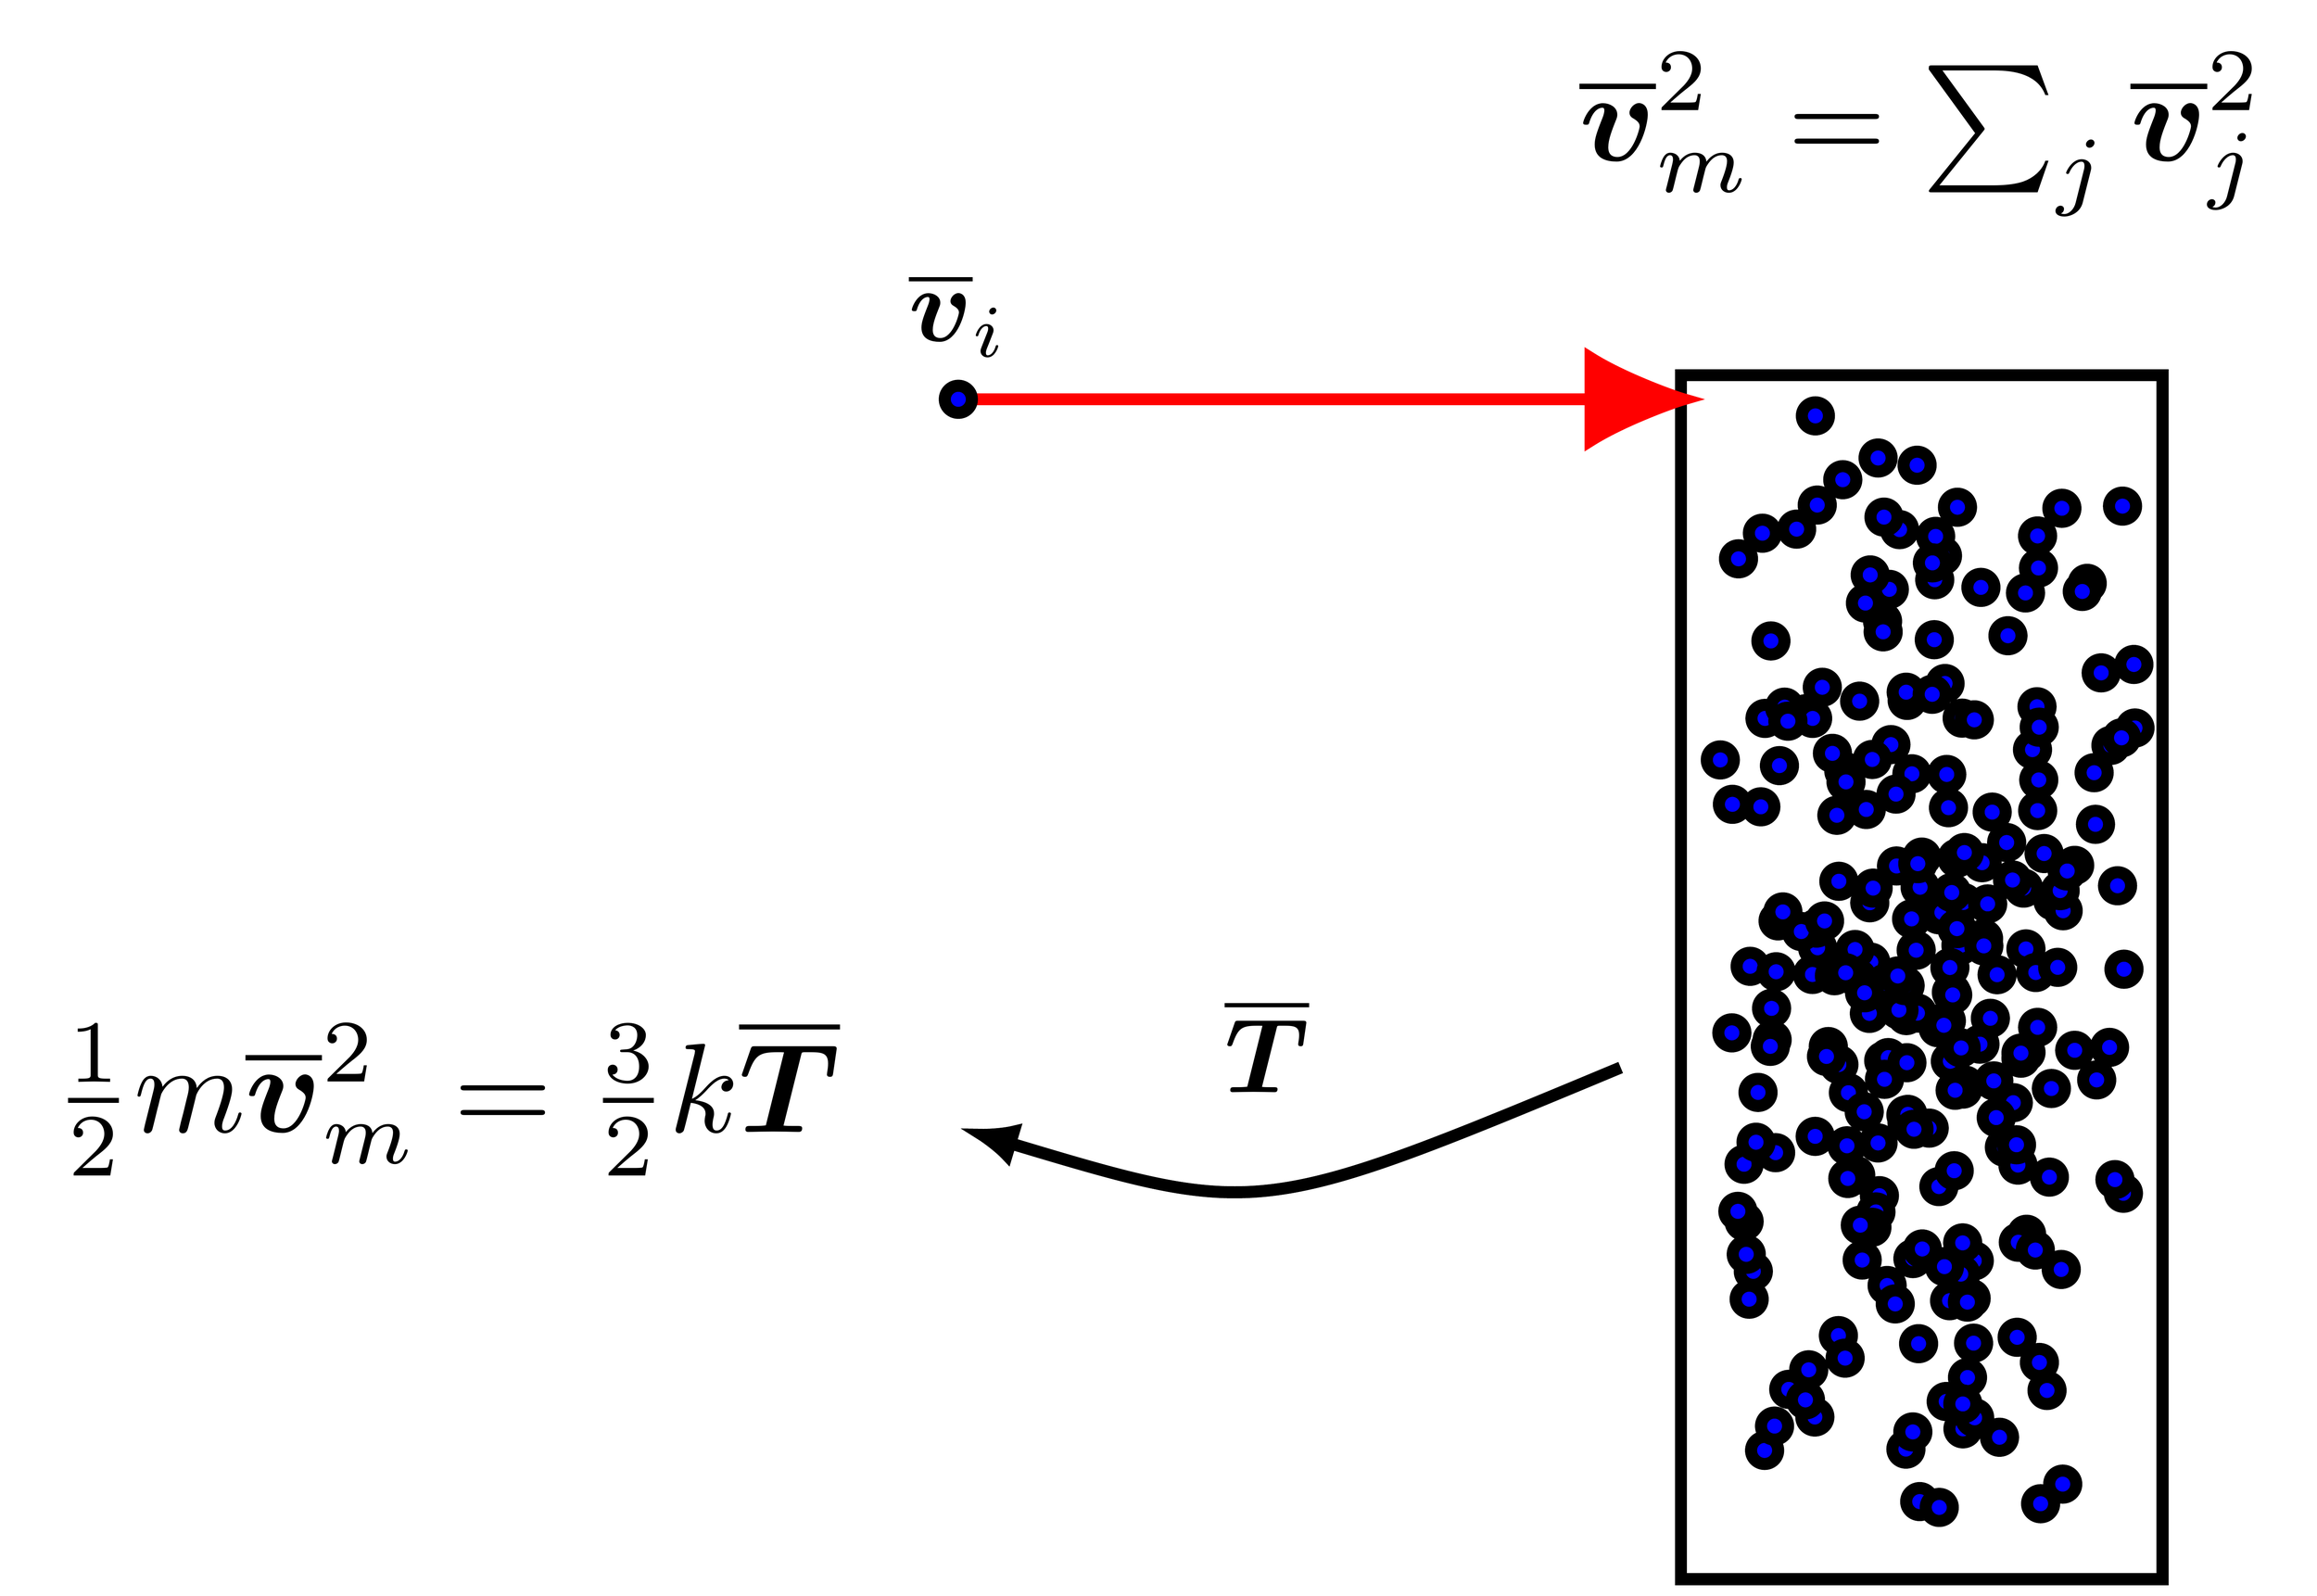
\begin{tikzpicture}[>=latex,node distance=0pt, line width=4mm]

    \begin{scope}[yshift=7 cm, xshift=40cm, start chain=going right, scale=4.0]
      \draw [fill=none] (-2,-5) --  (2,-5) --  (2,5) -- (-2,5) -- cycle;

     \foreach \d in {1,2,3}{
      \foreach \y in {2,4,5,7,8,8.2,8.5,9,9.5,9}{
       \foreach \x in {2,4,5,7,8,8.5,9,9}{
        \node [fill=blue, draw=black, circle, inner sep=0pt, minimum size=0.3cm,scale=3] at (rand*\x*0.2,rand*\y*0.5) {};
       }
      }
     } 
     \node [fill=none, draw=none, inner sep=0pt, minimum size=0.3cm,scale=10] at (-8.0,+5.5) {$\overline{\bm{v}}_i$};
     \draw[-{Latex[length=40mm,width=35mm]},draw=Red] (-8.0,+4.8) -- (-1.8,+4.8) ;
     \node [fill=blue, draw=black, circle, inner sep=0pt, minimum size=0.3cm,scale=3] at (-8.0,+4.8) {};
    \end{scope}

    \draw[{Latex[length=20mm,width=15mm]}-] (8,2) .. controls ++(10,-3) .. 
    node[above, scale=10] {$\overline{\bm{T}}$}
    ++(22,+2);

    \node[scale=12] at (-9,3) {$\frac{1}{2}m\overline{\bm{v}}_{m}^2 = \frac{3}{2}k\overline{\bm{T}}$};
    \node[scale=12] at (40,35) {$\overline{\bm{v}}_{m}^2 = \sum_j \overline{\bm{v}}_j^2$};

\end{tikzpicture}

\end{document}

}
%\end{figure}
%\end{frame}

%------------------------------------------------

\begin{frame}
\frametitle{The micro-problem in the FE$^2$ method}
\begin{figure}[!ht]
\resizebox{0.8\linewidth}{!}{\documentclass{standalone}

\begin{document}

\tikzset{cross/.style={cross out, draw=black, fill=none, minimum size=2*(#1-\pgflinewidth), inner sep=0pt, outer
sep=0pt}, cross/.default={2pt}}

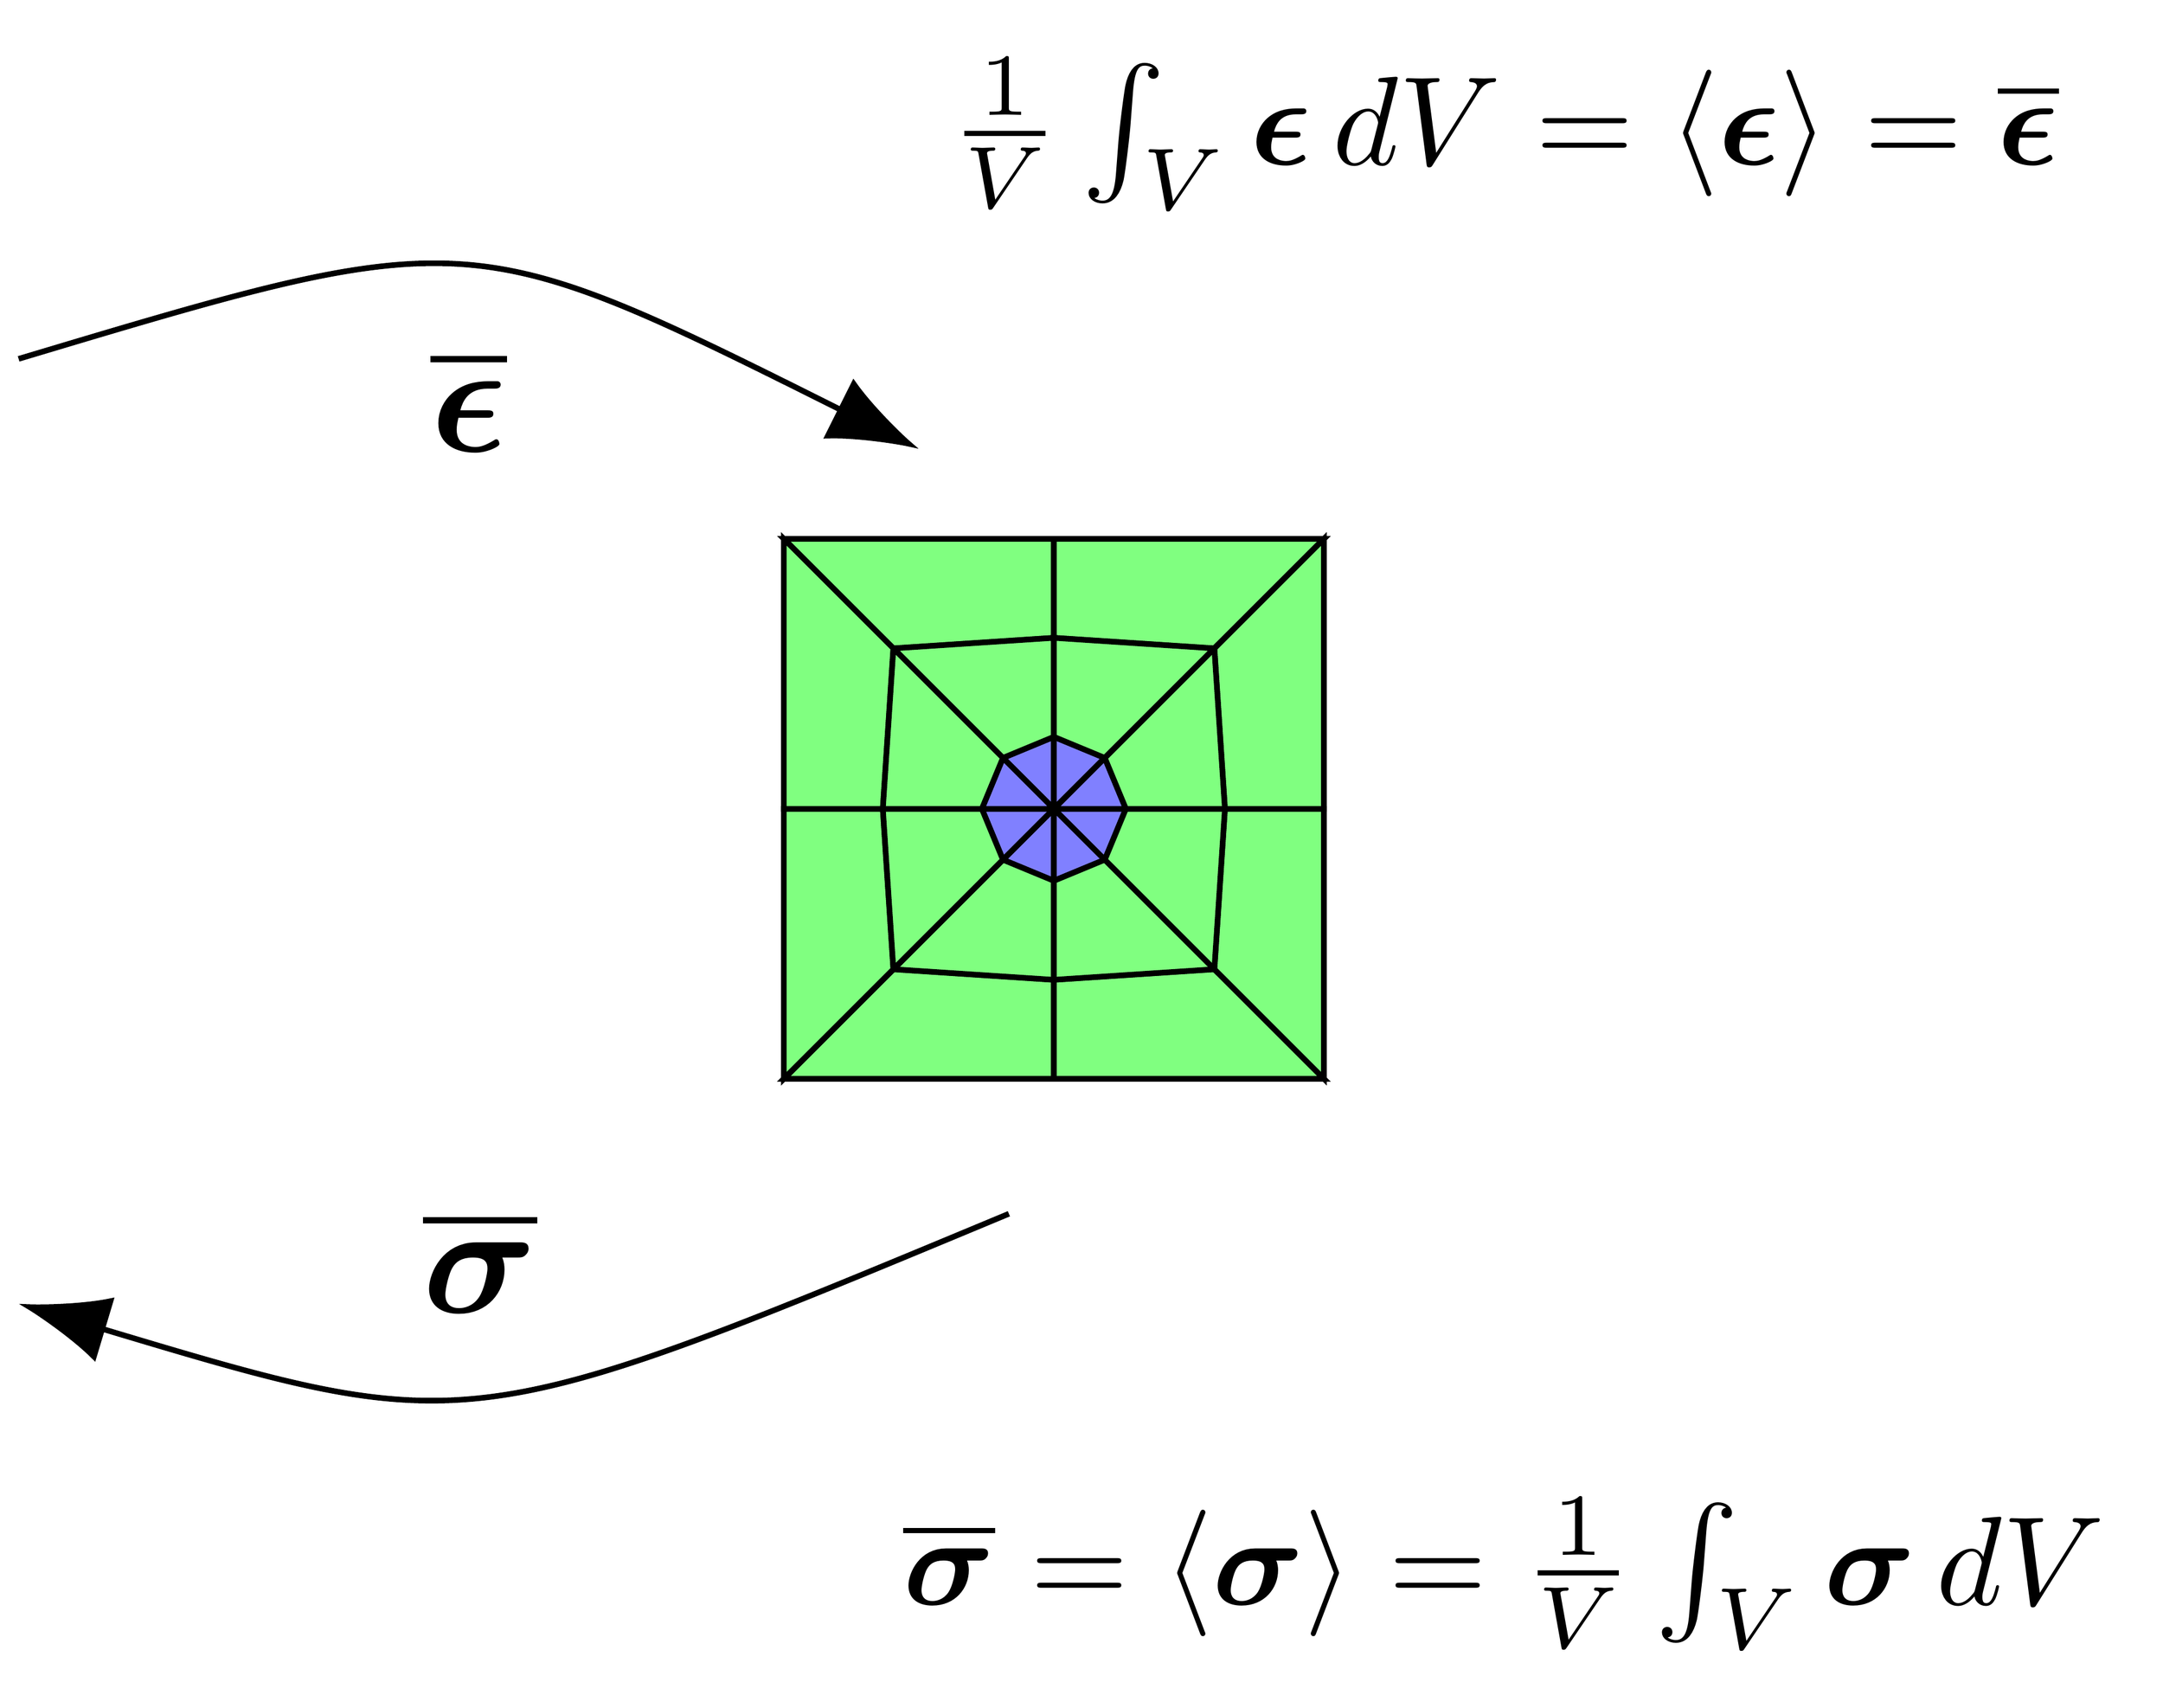
\begin{tikzpicture}[>=latex,node distance=0pt, line width=1.25mm]

    \begin{scope}[yshift=7 cm, xshift=40cm, start chain=going right, scale=4.0]
      \coordinate [draw=black,shift={(0,0)}] (0) at (0,0);
      \coordinate [draw=black,shift={(0,0)}] (1) at (1.5,0);
      \coordinate [draw=black,shift={(0,0)}] (2) at (1.5,1.5);
      \coordinate [draw=black,shift={(0,0)}] (3) at (1.5,1.1);
      \coordinate [draw=black,shift={(0,0)}] (4) at (1.2171572876,1.2171572876);
      \coordinate [draw=black,shift={(0,0)}] (5) at (1.1,1.5);
      \coordinate [draw=black,shift={(0,0)}] (6) at (0,1.5);
      \coordinate [draw=black,shift={(0,0)}] (7) at (0,3);
      \coordinate [draw=black,shift={(0,0)}] (8) at (1.2171572876,1.7828427124);
      \coordinate [draw=black,shift={(0,0)}] (9) at (1.5,1.9);
      \coordinate [draw=black,shift={(0,0)}] (10) at (1.5,3);
      \coordinate [draw=black,shift={(0,0)}] (11) at (3,0);
      \coordinate [draw=black,shift={(0,0)}] (12) at (1.7828427124,1.2171572876);
      \coordinate [draw=black,shift={(0,0)}] (13) at (1.9,1.5);
      \coordinate [draw=black,shift={(0,0)}] (14) at (3,1.5);
      \coordinate [draw=black,shift={(0,0)}] (15) at (3,3);
      \coordinate [draw=black,shift={(0,0)}] (16) at (1.7828427124,1.7828427124);
      \coordinate [draw=black,shift={(0,0)}] (17) at (1.5,0.5500000000014312);
      \coordinate [draw=black,shift={(0,0)}] (18) at (0.6085786437983935,0.6085786437983935);
      \coordinate [draw=black,shift={(0,0)}] (19) at (0.5500000000014312,1.5);
      \coordinate [draw=black,shift={(0,0)}] (20) at (0.6085786437983723,2.391421356201628);
      \coordinate [draw=black,shift={(0,0)}] (21) at (1.5,2.449999999998004);
      \coordinate [draw=black,shift={(0,0)}] (22) at (2.391421356201628,0.6085786437983723);
      \coordinate [draw=black,shift={(0,0)}] (23) at (2.449999999998004,1.5);
      \coordinate [draw=black,shift={(0,0)}] (24) at (2.391421356201648,2.391421356201648);
      \draw [fill=blue!50] (2) --  (4) --  (3) -- cycle;
      \draw [fill=blue!50] (2) --  (4) --  (5) -- cycle;
      \draw [fill=blue!50] (2) --  (8) --  (9) -- cycle;
      \draw [fill=blue!50] (2) --  (8) --  (5) -- cycle;
      \draw [fill=blue!50] (2) --  (12) --  (3) -- cycle;
      \draw [fill=blue!50] (2) --  (12) --  (13) -- cycle;
      \draw [fill=blue!50] (2) --  (16) --  (9) -- cycle;
      \draw [fill=blue!50] (2) --  (16) --  (13) -- cycle;
      \draw [fill=green!50] (0) --  (18) --  (17) --  (1) -- cycle;
      \draw [fill=green!50] (18) --  (4) --  (3) --  (17) -- cycle;
      \draw [fill=green!50] (0) --  (18) --  (19) --  (6) -- cycle;
      \draw [fill=green!50] (18) --  (4) --  (5) --  (19) -- cycle;
      \draw [fill=green!50] (7) --  (20) --  (21) --  (10) -- cycle;
      \draw [fill=green!50] (20) --  (8) --  (9) --  (21) -- cycle;
      \draw [fill=green!50] (7) --  (20) --  (19) --  (6) -- cycle;
      \draw [fill=green!50] (20) --  (8) --  (5) --  (19) -- cycle;
      \draw [fill=green!50] (11) --  (22) --  (17) --  (1) -- cycle;
      \draw [fill=green!50] (22) --  (12) --  (3) --  (17) -- cycle;
      \draw [fill=green!50] (11) --  (22) --  (23) --  (14) -- cycle;
      \draw [fill=green!50] (22) --  (12) --  (13) --  (23) -- cycle;
      \draw [fill=green!50] (15) --  (24) --  (21) --  (10) -- cycle;
      \draw [fill=green!50] (24) --  (16) --  (9) --  (21) -- cycle;
      \draw [fill=green!50] (15) --  (24) --  (23) --  (14) -- cycle;
      \draw [fill=green!50] (24) --  (16) --  (13) --  (23) -- cycle;
      \node [fill=black, draw=none, circle, inner sep=0pt, minimum size=0.1cm,scale=0.3] at (0) {h};
      \node [fill=black, draw=none, circle, inner sep=0pt, minimum size=0.1cm,scale=0.3] at (1) {h};
      \node [fill=black, draw=none, circle, inner sep=0pt, minimum size=0.1cm,scale=0.3] at (2) {h};
      \node [fill=black, draw=none, circle, inner sep=0pt, minimum size=0.1cm,scale=0.3] at (3) {h};
      \node [fill=black, draw=none, circle, inner sep=0pt, minimum size=0.1cm,scale=0.3] at (4) {h};
      \node [fill=black, draw=none, circle, inner sep=0pt, minimum size=0.1cm,scale=0.3] at (5) {h};
      \node [fill=black, draw=none, circle, inner sep=0pt, minimum size=0.1cm,scale=0.3] at (6) {h};
      \node [fill=black, draw=none, circle, inner sep=0pt, minimum size=0.1cm,scale=0.3] at (7) {h};
      \node [fill=black, draw=none, circle, inner sep=0pt, minimum size=0.1cm,scale=0.3] at (8) {h};
      \node [fill=black, draw=none, circle, inner sep=0pt, minimum size=0.1cm,scale=0.3] at (9) {h};
      \node [fill=black, draw=none, circle, inner sep=0pt, minimum size=0.1cm,scale=0.3] at (10) {h};
      \node [fill=black, draw=none, circle, inner sep=0pt, minimum size=0.1cm,scale=0.3] at (11) {h};
      \node [fill=black, draw=none, circle, inner sep=0pt, minimum size=0.1cm,scale=0.3] at (12) {h};
      \node [fill=black, draw=none, circle, inner sep=0pt, minimum size=0.1cm,scale=0.3] at (13) {h};
      \node [fill=black, draw=none, circle, inner sep=0pt, minimum size=0.1cm,scale=0.3] at (14) {h};
      \node [fill=black, draw=none, circle, inner sep=0pt, minimum size=0.1cm,scale=0.3] at (15) {h};
      \node [fill=black, draw=none, circle, inner sep=0pt, minimum size=0.1cm,scale=0.3] at (16) {h};
      \node [fill=black, draw=none, circle, inner sep=0pt, minimum size=0.1cm,scale=0.3] at (17) {h};
      \node [fill=black, draw=none, circle, inner sep=0pt, minimum size=0.1cm,scale=0.3] at (18) {h};
      \node [fill=black, draw=none, circle, inner sep=0pt, minimum size=0.1cm,scale=0.3] at (19) {h};
      \node [fill=black, draw=none, circle, inner sep=0pt, minimum size=0.1cm,scale=0.3] at (20) {h};
      \node [fill=black, draw=none, circle, inner sep=0pt, minimum size=0.1cm,scale=0.3] at (21) {h};
      \node [fill=black, draw=none, circle, inner sep=0pt, minimum size=0.1cm,scale=0.3] at (22) {h};
      \node [fill=black, draw=none, circle, inner sep=0pt, minimum size=0.1cm,scale=0.3] at (23) {h};
      \node [fill=black, draw=none, circle, inner sep=0pt, minimum size=0.1cm,scale=0.3] at (24) {h};
    \end{scope}

    \draw[-{Latex[length=20mm,width=15mm]}] (23,23) ..  controls ++(10,+3) ..
    node[below, scale=10] {$\overline{\bm{\epsilon}}$} 
    ++(20,-2);
    \draw[{Latex[length=20mm,width=15mm]}-] (23,2) .. controls ++(10,-3) .. 
    node[above, scale=10] {$\overline{\bm{\sigma}}$}
    ++(22,+2);

    \node[scale=8] at (56,-4) {$\overline{\bm{\sigma}} = \langle \bm{\sigma} \rangle= \frac{1}{V} \int_{V} \bm{\sigma} \, dV$} ;
    \node[scale=8] at (56,28) {$\frac{1}{V} \int_{V} \bm{\epsilon} \, dV = \langle \bm{\epsilon} \rangle = \overline{\bm{\epsilon}}$} ;

\end{tikzpicture}

\end{document}

}
\end{figure}
\end{frame}

%------------------------------------------------

\begin{frame}
\frametitle{The micro-problem in the FE$^2$ method}
\begin{figure}[!ht]
\resizebox{0.8\linewidth}{!}{\documentclass{standalone}

\begin{document}

\tikzset{cross/.style={cross out, draw=black, fill=none, minimum size=2*(#1-\pgflinewidth), inner sep=0pt, outer
sep=0pt}, cross/.default={2pt}}

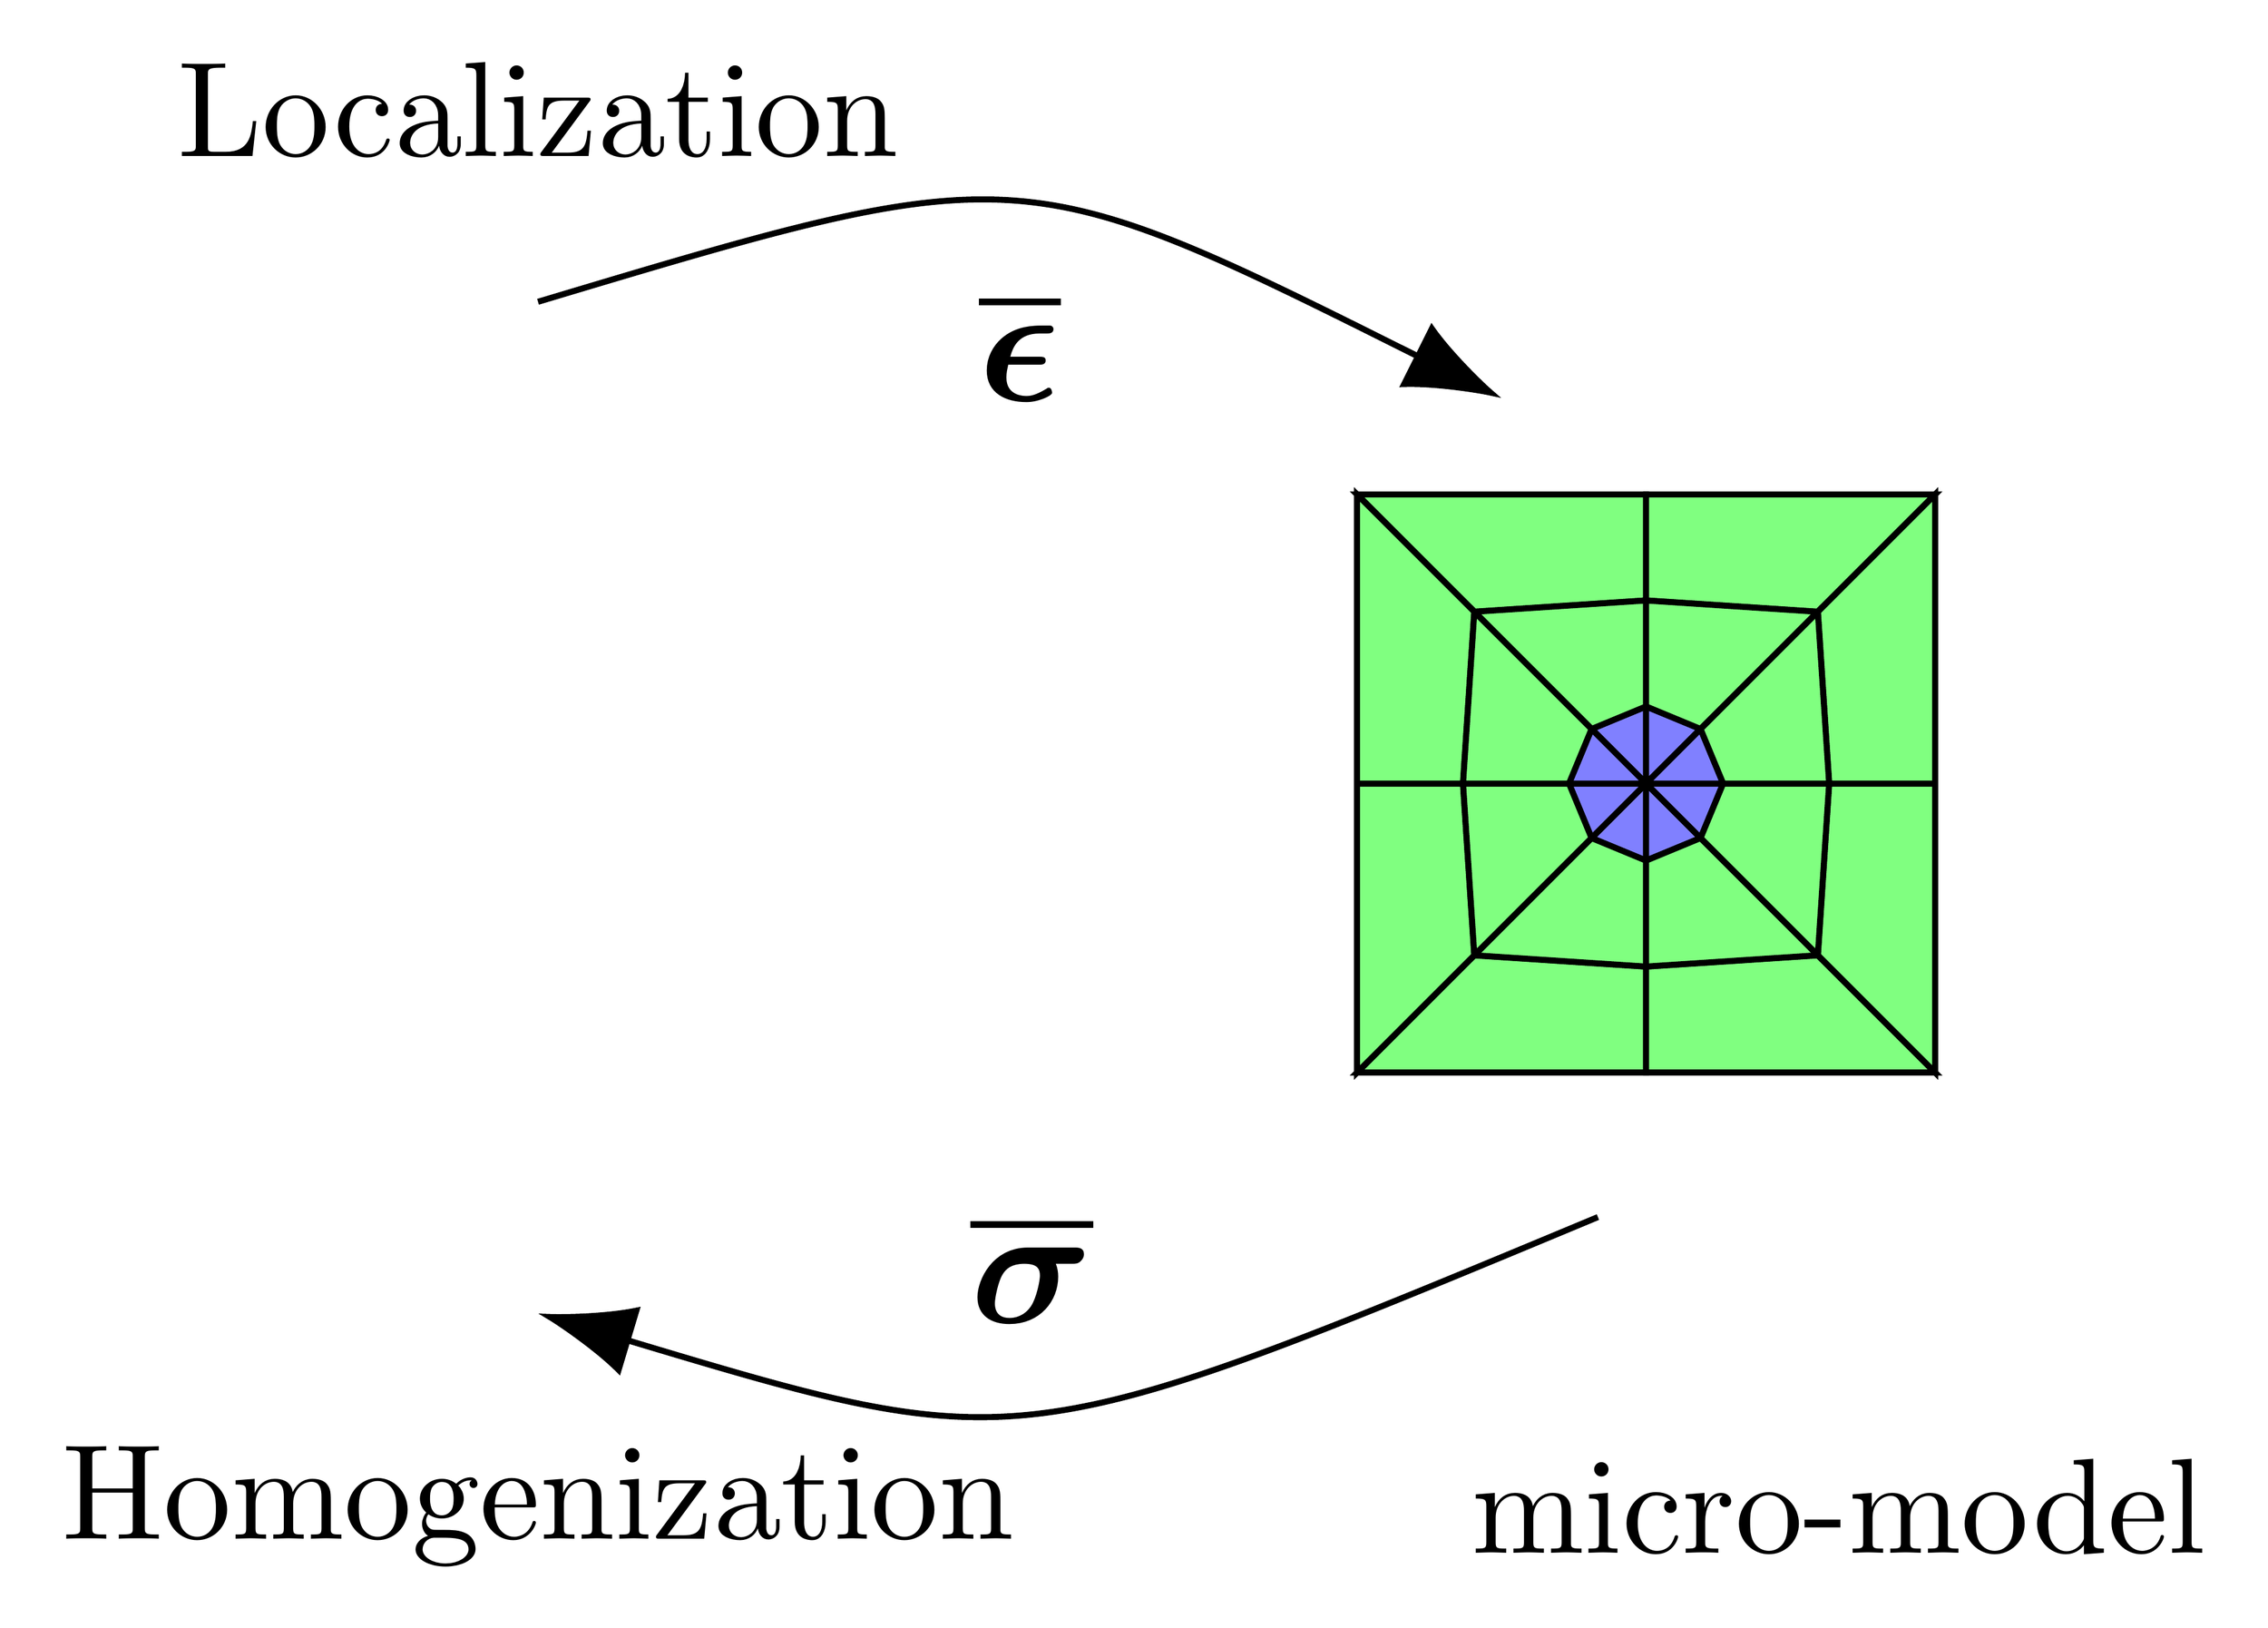
\begin{tikzpicture}[>=latex,node distance=0pt, line width=1.25mm]

    \begin{scope}[yshift=7 cm, xshift=40cm, start chain=going right, scale=4.0]
      \coordinate [draw=black,shift={(0,0)}] (0) at (0,0);
      \coordinate [draw=black,shift={(0,0)}] (1) at (1.5,0);
      \coordinate [draw=black,shift={(0,0)}] (2) at (1.5,1.5);
      \coordinate [draw=black,shift={(0,0)}] (3) at (1.5,1.1);
      \coordinate [draw=black,shift={(0,0)}] (4) at (1.2171572876,1.2171572876);
      \coordinate [draw=black,shift={(0,0)}] (5) at (1.1,1.5);
      \coordinate [draw=black,shift={(0,0)}] (6) at (0,1.5);
      \coordinate [draw=black,shift={(0,0)}] (7) at (0,3);
      \coordinate [draw=black,shift={(0,0)}] (8) at (1.2171572876,1.7828427124);
      \coordinate [draw=black,shift={(0,0)}] (9) at (1.5,1.9);
      \coordinate [draw=black,shift={(0,0)}] (10) at (1.5,3);
      \coordinate [draw=black,shift={(0,0)}] (11) at (3,0);
      \coordinate [draw=black,shift={(0,0)}] (12) at (1.7828427124,1.2171572876);
      \coordinate [draw=black,shift={(0,0)}] (13) at (1.9,1.5);
      \coordinate [draw=black,shift={(0,0)}] (14) at (3,1.5);
      \coordinate [draw=black,shift={(0,0)}] (15) at (3,3);
      \coordinate [draw=black,shift={(0,0)}] (16) at (1.7828427124,1.7828427124);
      \coordinate [draw=black,shift={(0,0)}] (17) at (1.5,0.5500000000014312);
      \coordinate [draw=black,shift={(0,0)}] (18) at (0.6085786437983935,0.6085786437983935);
      \coordinate [draw=black,shift={(0,0)}] (19) at (0.5500000000014312,1.5);
      \coordinate [draw=black,shift={(0,0)}] (20) at (0.6085786437983723,2.391421356201628);
      \coordinate [draw=black,shift={(0,0)}] (21) at (1.5,2.449999999998004);
      \coordinate [draw=black,shift={(0,0)}] (22) at (2.391421356201628,0.6085786437983723);
      \coordinate [draw=black,shift={(0,0)}] (23) at (2.449999999998004,1.5);
      \coordinate [draw=black,shift={(0,0)}] (24) at (2.391421356201648,2.391421356201648);
      \draw [fill=blue!50] (2) --  (4) --  (3) -- cycle;
      \draw [fill=blue!50] (2) --  (4) --  (5) -- cycle;
      \draw [fill=blue!50] (2) --  (8) --  (9) -- cycle;
      \draw [fill=blue!50] (2) --  (8) --  (5) -- cycle;
      \draw [fill=blue!50] (2) --  (12) --  (3) -- cycle;
      \draw [fill=blue!50] (2) --  (12) --  (13) -- cycle;
      \draw [fill=blue!50] (2) --  (16) --  (9) -- cycle;
      \draw [fill=blue!50] (2) --  (16) --  (13) -- cycle;
      \draw [fill=green!50] (0) --  (18) --  (17) --  (1) -- cycle;
      \draw [fill=green!50] (18) --  (4) --  (3) --  (17) -- cycle;
      \draw [fill=green!50] (0) --  (18) --  (19) --  (6) -- cycle;
      \draw [fill=green!50] (18) --  (4) --  (5) --  (19) -- cycle;
      \draw [fill=green!50] (7) --  (20) --  (21) --  (10) -- cycle;
      \draw [fill=green!50] (20) --  (8) --  (9) --  (21) -- cycle;
      \draw [fill=green!50] (7) --  (20) --  (19) --  (6) -- cycle;
      \draw [fill=green!50] (20) --  (8) --  (5) --  (19) -- cycle;
      \draw [fill=green!50] (11) --  (22) --  (17) --  (1) -- cycle;
      \draw [fill=green!50] (22) --  (12) --  (3) --  (17) -- cycle;
      \draw [fill=green!50] (11) --  (22) --  (23) --  (14) -- cycle;
      \draw [fill=green!50] (22) --  (12) --  (13) --  (23) -- cycle;
      \draw [fill=green!50] (15) --  (24) --  (21) --  (10) -- cycle;
      \draw [fill=green!50] (24) --  (16) --  (9) --  (21) -- cycle;
      \draw [fill=green!50] (15) --  (24) --  (23) --  (14) -- cycle;
      \draw [fill=green!50] (24) --  (16) --  (13) --  (23) -- cycle;
      \node [fill=black, draw=none, circle, inner sep=0pt, minimum size=0.1cm,scale=0.3] at (0) {h};
      \node [fill=black, draw=none, circle, inner sep=0pt, minimum size=0.1cm,scale=0.3] at (1) {h};
      \node [fill=black, draw=none, circle, inner sep=0pt, minimum size=0.1cm,scale=0.3] at (2) {h};
      \node [fill=black, draw=none, circle, inner sep=0pt, minimum size=0.1cm,scale=0.3] at (3) {h};
      \node [fill=black, draw=none, circle, inner sep=0pt, minimum size=0.1cm,scale=0.3] at (4) {h};
      \node [fill=black, draw=none, circle, inner sep=0pt, minimum size=0.1cm,scale=0.3] at (5) {h};
      \node [fill=black, draw=none, circle, inner sep=0pt, minimum size=0.1cm,scale=0.3] at (6) {h};
      \node [fill=black, draw=none, circle, inner sep=0pt, minimum size=0.1cm,scale=0.3] at (7) {h};
      \node [fill=black, draw=none, circle, inner sep=0pt, minimum size=0.1cm,scale=0.3] at (8) {h};
      \node [fill=black, draw=none, circle, inner sep=0pt, minimum size=0.1cm,scale=0.3] at (9) {h};
      \node [fill=black, draw=none, circle, inner sep=0pt, minimum size=0.1cm,scale=0.3] at (10) {h};
      \node [fill=black, draw=none, circle, inner sep=0pt, minimum size=0.1cm,scale=0.3] at (11) {h};
      \node [fill=black, draw=none, circle, inner sep=0pt, minimum size=0.1cm,scale=0.3] at (12) {h};
      \node [fill=black, draw=none, circle, inner sep=0pt, minimum size=0.1cm,scale=0.3] at (13) {h};
      \node [fill=black, draw=none, circle, inner sep=0pt, minimum size=0.1cm,scale=0.3] at (14) {h};
      \node [fill=black, draw=none, circle, inner sep=0pt, minimum size=0.1cm,scale=0.3] at (15) {h};
      \node [fill=black, draw=none, circle, inner sep=0pt, minimum size=0.1cm,scale=0.3] at (16) {h};
      \node [fill=black, draw=none, circle, inner sep=0pt, minimum size=0.1cm,scale=0.3] at (17) {h};
      \node [fill=black, draw=none, circle, inner sep=0pt, minimum size=0.1cm,scale=0.3] at (18) {h};
      \node [fill=black, draw=none, circle, inner sep=0pt, minimum size=0.1cm,scale=0.3] at (19) {h};
      \node [fill=black, draw=none, circle, inner sep=0pt, minimum size=0.1cm,scale=0.3] at (20) {h};
      \node [fill=black, draw=none, circle, inner sep=0pt, minimum size=0.1cm,scale=0.3] at (21) {h};
      \node [fill=black, draw=none, circle, inner sep=0pt, minimum size=0.1cm,scale=0.3] at (22) {h};
      \node [fill=black, draw=none, circle, inner sep=0pt, minimum size=0.1cm,scale=0.3] at (23) {h};
      \node [fill=black, draw=none, circle, inner sep=0pt, minimum size=0.1cm,scale=0.3] at (24) {h};
    \end{scope}

    \draw[-{Latex[length=20mm,width=15mm]}] (23,23) ..  controls ++(10,+3) ..
    node[below, scale=10] {$\overline{\bm{\epsilon}}$} 
    ++(20,-2);
    \draw[{Latex[length=20mm,width=15mm]}-] (23,2) .. controls ++(10,-3) .. 
    node[above, scale=10] {$\overline{\bm{\sigma}}$}
    ++(22,+2);

    \node[scale=8] at (23,-2) {Homogenization};
    \node[scale=8] at (23,27) {Localization};

    \node[scale=8] at (50,-2) {micro-model};

\end{tikzpicture}

\end{document}

}
\end{figure}
\end{frame}

%------------------------------------------------

\begin{frame}
\frametitle{The micro-problem in the FE$^2$ method}
\begin{figure}[!ht]
\resizebox{1.0\linewidth}{!}{\documentclass{standalone}

\begin{document}

\tikzset{cross/.style={cross out, draw=black, fill=none, minimum size=2*(#1-\pgflinewidth), inner sep=0pt, outer
sep=0pt}, cross/.default={2pt}}

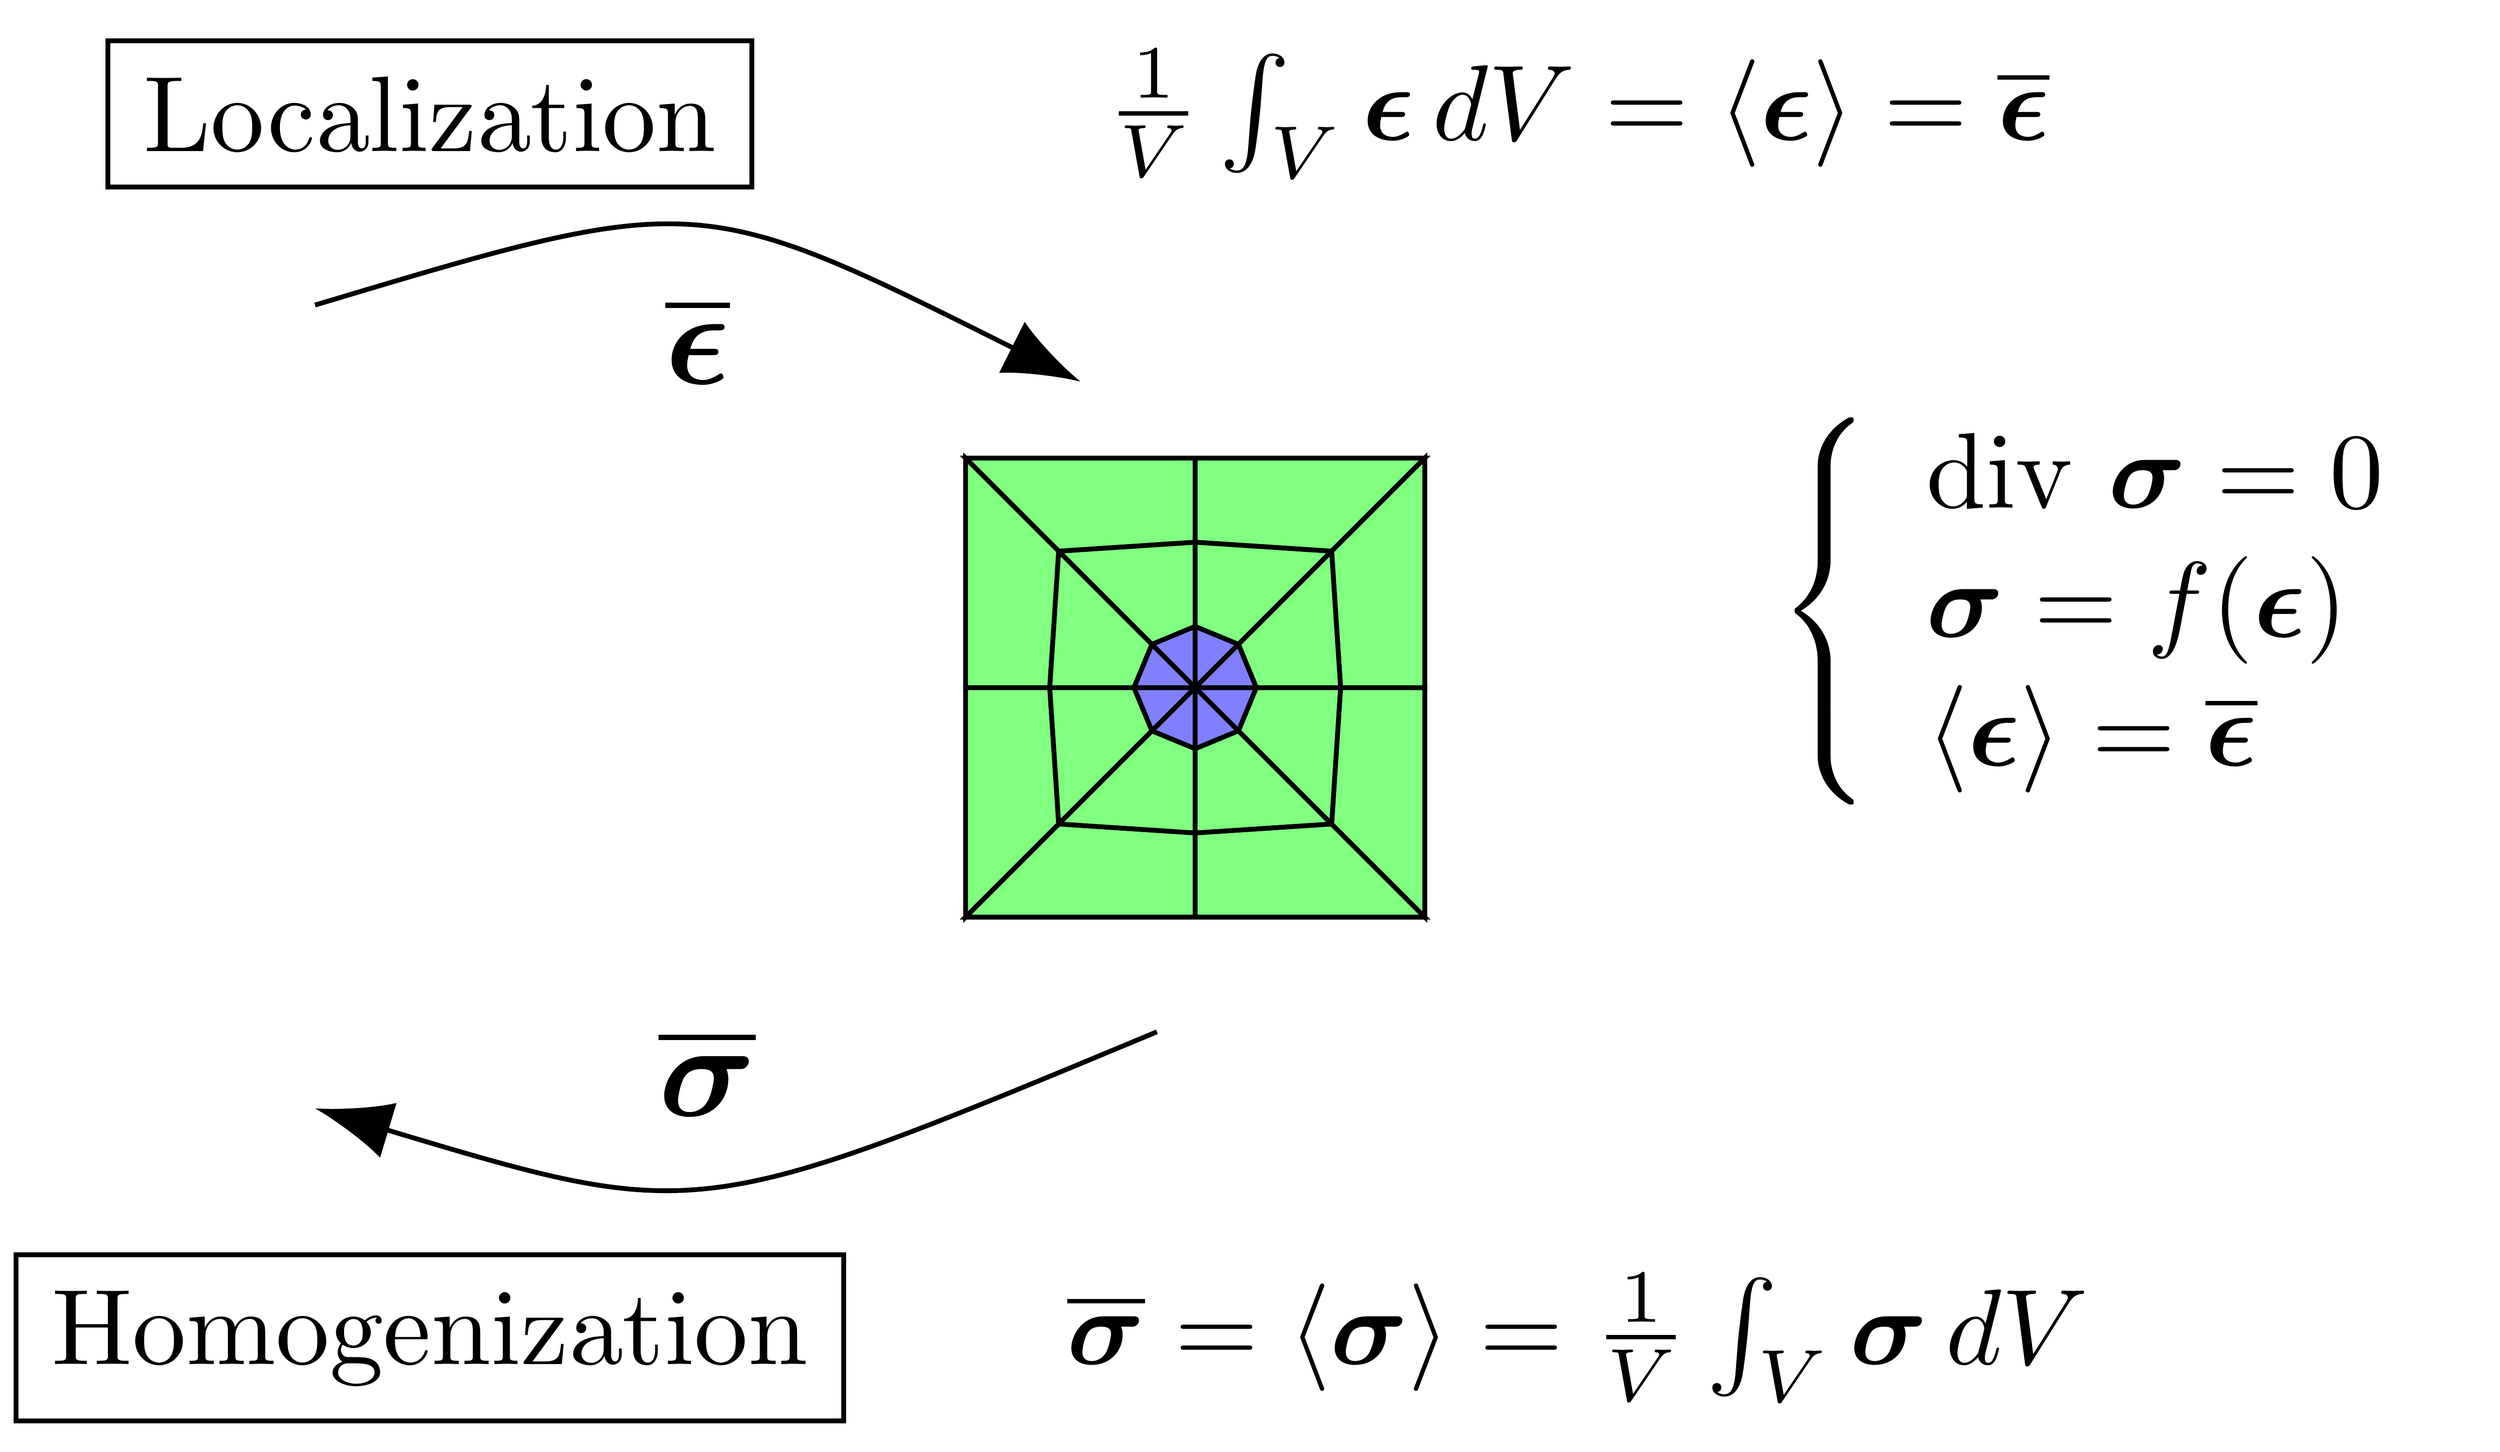
\begin{tikzpicture}[>=latex,node distance=0pt, line width=1.25mm]

    \begin{scope}[yshift=7 cm, xshift=40cm, start chain=going right, scale=4.0]
      \coordinate [draw=black,shift={(0,0)}] (0) at (0,0);
      \coordinate [draw=black,shift={(0,0)}] (1) at (1.5,0);
      \coordinate [draw=black,shift={(0,0)}] (2) at (1.5,1.5);
      \coordinate [draw=black,shift={(0,0)}] (3) at (1.5,1.1);
      \coordinate [draw=black,shift={(0,0)}] (4) at (1.2171572876,1.2171572876);
      \coordinate [draw=black,shift={(0,0)}] (5) at (1.1,1.5);
      \coordinate [draw=black,shift={(0,0)}] (6) at (0,1.5);
      \coordinate [draw=black,shift={(0,0)}] (7) at (0,3);
      \coordinate [draw=black,shift={(0,0)}] (8) at (1.2171572876,1.7828427124);
      \coordinate [draw=black,shift={(0,0)}] (9) at (1.5,1.9);
      \coordinate [draw=black,shift={(0,0)}] (10) at (1.5,3);
      \coordinate [draw=black,shift={(0,0)}] (11) at (3,0);
      \coordinate [draw=black,shift={(0,0)}] (12) at (1.7828427124,1.2171572876);
      \coordinate [draw=black,shift={(0,0)}] (13) at (1.9,1.5);
      \coordinate [draw=black,shift={(0,0)}] (14) at (3,1.5);
      \coordinate [draw=black,shift={(0,0)}] (15) at (3,3);
      \coordinate [draw=black,shift={(0,0)}] (16) at (1.7828427124,1.7828427124);
      \coordinate [draw=black,shift={(0,0)}] (17) at (1.5,0.5500000000014312);
      \coordinate [draw=black,shift={(0,0)}] (18) at (0.6085786437983935,0.6085786437983935);
      \coordinate [draw=black,shift={(0,0)}] (19) at (0.5500000000014312,1.5);
      \coordinate [draw=black,shift={(0,0)}] (20) at (0.6085786437983723,2.391421356201628);
      \coordinate [draw=black,shift={(0,0)}] (21) at (1.5,2.449999999998004);
      \coordinate [draw=black,shift={(0,0)}] (22) at (2.391421356201628,0.6085786437983723);
      \coordinate [draw=black,shift={(0,0)}] (23) at (2.449999999998004,1.5);
      \coordinate [draw=black,shift={(0,0)}] (24) at (2.391421356201648,2.391421356201648);
      \draw [fill=blue!50] (2) --  (4) --  (3) -- cycle;
      \draw [fill=blue!50] (2) --  (4) --  (5) -- cycle;
      \draw [fill=blue!50] (2) --  (8) --  (9) -- cycle;
      \draw [fill=blue!50] (2) --  (8) --  (5) -- cycle;
      \draw [fill=blue!50] (2) --  (12) --  (3) -- cycle;
      \draw [fill=blue!50] (2) --  (12) --  (13) -- cycle;
      \draw [fill=blue!50] (2) --  (16) --  (9) -- cycle;
      \draw [fill=blue!50] (2) --  (16) --  (13) -- cycle;
      \draw [fill=green!50] (0) --  (18) --  (17) --  (1) -- cycle;
      \draw [fill=green!50] (18) --  (4) --  (3) --  (17) -- cycle;
      \draw [fill=green!50] (0) --  (18) --  (19) --  (6) -- cycle;
      \draw [fill=green!50] (18) --  (4) --  (5) --  (19) -- cycle;
      \draw [fill=green!50] (7) --  (20) --  (21) --  (10) -- cycle;
      \draw [fill=green!50] (20) --  (8) --  (9) --  (21) -- cycle;
      \draw [fill=green!50] (7) --  (20) --  (19) --  (6) -- cycle;
      \draw [fill=green!50] (20) --  (8) --  (5) --  (19) -- cycle;
      \draw [fill=green!50] (11) --  (22) --  (17) --  (1) -- cycle;
      \draw [fill=green!50] (22) --  (12) --  (3) --  (17) -- cycle;
      \draw [fill=green!50] (11) --  (22) --  (23) --  (14) -- cycle;
      \draw [fill=green!50] (22) --  (12) --  (13) --  (23) -- cycle;
      \draw [fill=green!50] (15) --  (24) --  (21) --  (10) -- cycle;
      \draw [fill=green!50] (24) --  (16) --  (9) --  (21) -- cycle;
      \draw [fill=green!50] (15) --  (24) --  (23) --  (14) -- cycle;
      \draw [fill=green!50] (24) --  (16) --  (13) --  (23) -- cycle;
      \node [fill=black, draw=none, circle, inner sep=0pt, minimum size=0.1cm,scale=0.3] at (0) {h};
      \node [fill=black, draw=none, circle, inner sep=0pt, minimum size=0.1cm,scale=0.3] at (1) {h};
      \node [fill=black, draw=none, circle, inner sep=0pt, minimum size=0.1cm,scale=0.3] at (2) {h};
      \node [fill=black, draw=none, circle, inner sep=0pt, minimum size=0.1cm,scale=0.3] at (3) {h};
      \node [fill=black, draw=none, circle, inner sep=0pt, minimum size=0.1cm,scale=0.3] at (4) {h};
      \node [fill=black, draw=none, circle, inner sep=0pt, minimum size=0.1cm,scale=0.3] at (5) {h};
      \node [fill=black, draw=none, circle, inner sep=0pt, minimum size=0.1cm,scale=0.3] at (6) {h};
      \node [fill=black, draw=none, circle, inner sep=0pt, minimum size=0.1cm,scale=0.3] at (7) {h};
      \node [fill=black, draw=none, circle, inner sep=0pt, minimum size=0.1cm,scale=0.3] at (8) {h};
      \node [fill=black, draw=none, circle, inner sep=0pt, minimum size=0.1cm,scale=0.3] at (9) {h};
      \node [fill=black, draw=none, circle, inner sep=0pt, minimum size=0.1cm,scale=0.3] at (10) {h};
      \node [fill=black, draw=none, circle, inner sep=0pt, minimum size=0.1cm,scale=0.3] at (11) {h};
      \node [fill=black, draw=none, circle, inner sep=0pt, minimum size=0.1cm,scale=0.3] at (12) {h};
      \node [fill=black, draw=none, circle, inner sep=0pt, minimum size=0.1cm,scale=0.3] at (13) {h};
      \node [fill=black, draw=none, circle, inner sep=0pt, minimum size=0.1cm,scale=0.3] at (14) {h};
      \node [fill=black, draw=none, circle, inner sep=0pt, minimum size=0.1cm,scale=0.3] at (15) {h};
      \node [fill=black, draw=none, circle, inner sep=0pt, minimum size=0.1cm,scale=0.3] at (16) {h};
      \node [fill=black, draw=none, circle, inner sep=0pt, minimum size=0.1cm,scale=0.3] at (17) {h};
      \node [fill=black, draw=none, circle, inner sep=0pt, minimum size=0.1cm,scale=0.3] at (18) {h};
      \node [fill=black, draw=none, circle, inner sep=0pt, minimum size=0.1cm,scale=0.3] at (19) {h};
      \node [fill=black, draw=none, circle, inner sep=0pt, minimum size=0.1cm,scale=0.3] at (20) {h};
      \node [fill=black, draw=none, circle, inner sep=0pt, minimum size=0.1cm,scale=0.3] at (21) {h};
      \node [fill=black, draw=none, circle, inner sep=0pt, minimum size=0.1cm,scale=0.3] at (22) {h};
      \node [fill=black, draw=none, circle, inner sep=0pt, minimum size=0.1cm,scale=0.3] at (23) {h};
      \node [fill=black, draw=none, circle, inner sep=0pt, minimum size=0.1cm,scale=0.3] at (24) {h};
    \end{scope}

    \draw[-{Latex[length=20mm,width=15mm]}] (23,23) ..  controls ++(10,+3) ..
    node[below, scale=10] {$\overline{\bm{\epsilon}}$} 
    ++(20,-2);
    \draw[{Latex[length=20mm,width=15mm]}-] (23,2) .. controls ++(10,-3) .. 
    node[above, scale=10] {$\overline{\bm{\sigma}}$}
    ++(22,+2);

    \node[scale=8,draw=black] at (26,-4) {Homogenization};
    \node[scale=8,draw=black] at (26,28) {Localization};
    \node[scale=8] at (56,-4) {$\overline{\bm{\sigma}} = \langle \bm{\sigma} \rangle= \frac{1}{V} \int_{V} \bm{\sigma} \, dV$} ;
    \node[scale=8] at (56,28) {$\frac{1}{V} \int_{V} \bm{\epsilon} \, dV = \langle \bm{\epsilon} \rangle = \overline{\bm{\epsilon}}$} ;
    \node[scale=8] at (70,15) {$
    \left\{
    \begin{array}{ll}
    \text{div } \bm{\sigma} = 0 \\
    \bm{\sigma} = f(\bm{\epsilon}) \\
    \langle \bm{\epsilon} \rangle = \overline{\bm{\epsilon}}\\
    \end{array}
    \right.
    $};

\end{tikzpicture}

\end{document}

}
\end{figure}
\end{frame}

%------------------------------------------------

\begin{frame}
\frametitle{The best boundary conditions}
\begin{figure}[!ht]
\resizebox{0.6\linewidth}{!}{\documentclass{standalone}

\begin{document}

\tikzset{cross/.style={cross out, draw=black, fill=none, minimum size=2*(#1-\pgflinewidth), inner sep=0pt, outer
sep=0pt}, cross/.default={2pt}}

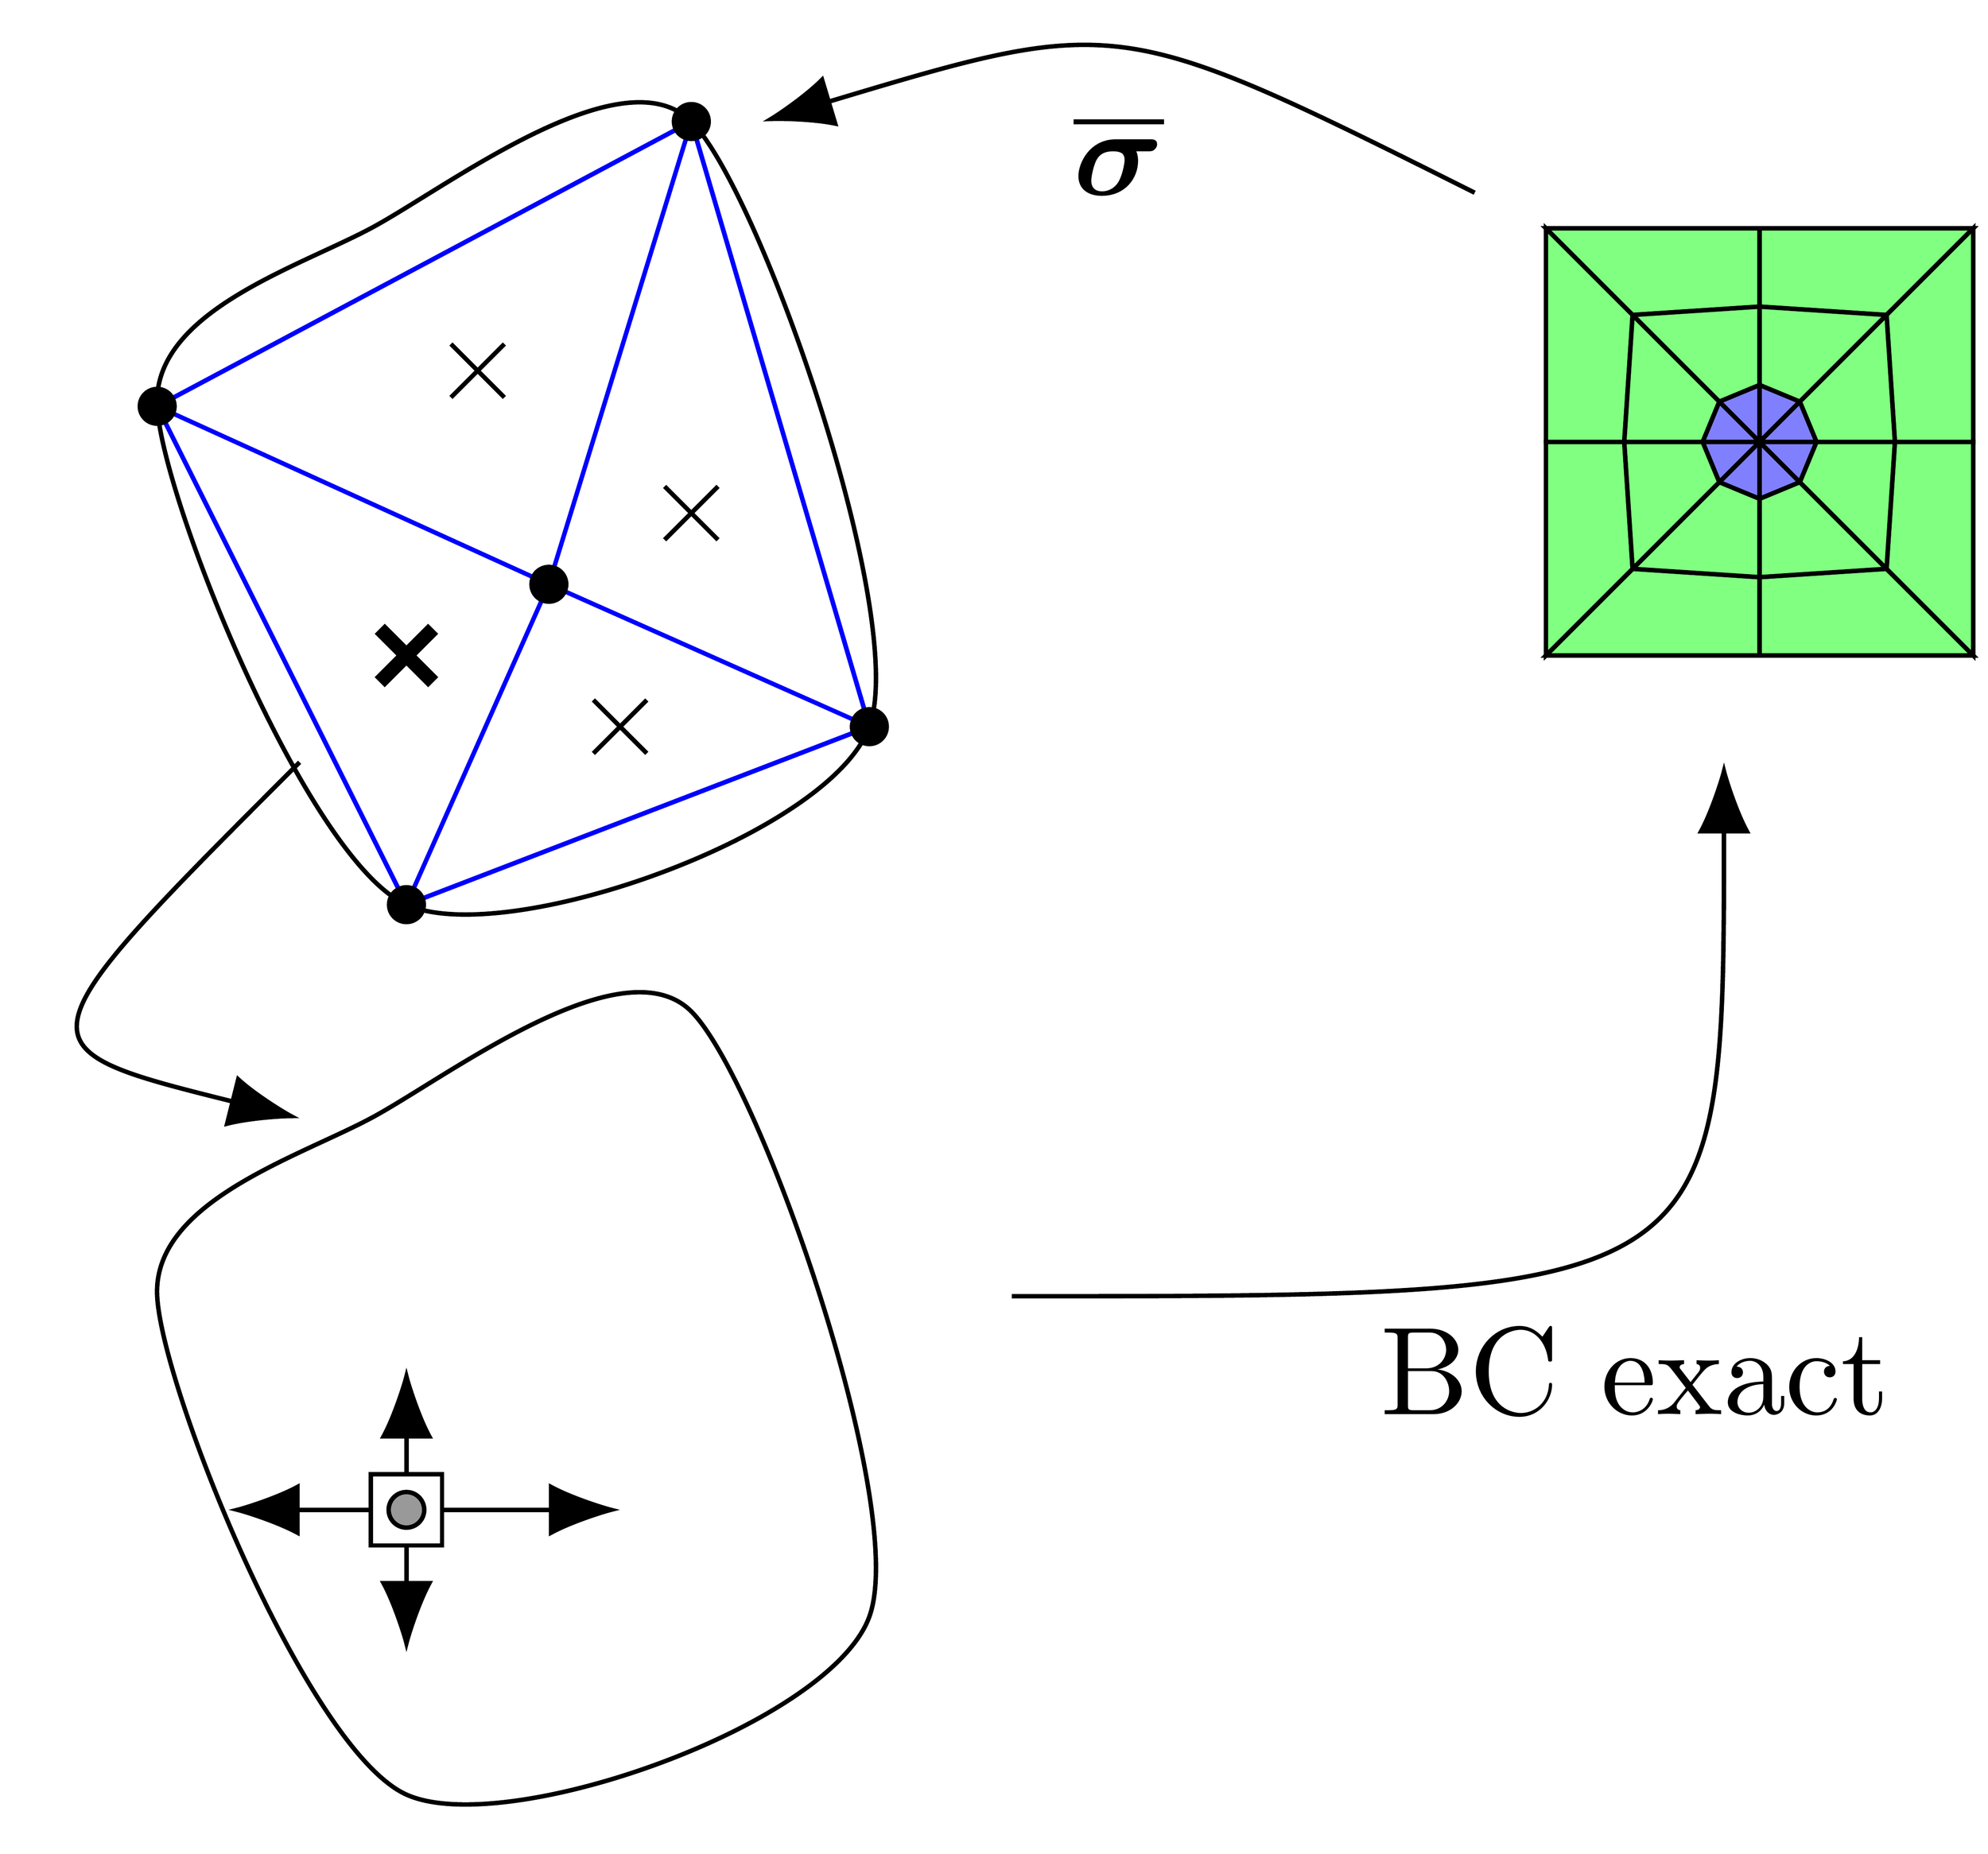
\begin{tikzpicture}[>=latex,node distance=0pt, line width=1.25mm]

% the h.m.s.

    \coordinate [draw=black,shift={(0,0)}] (0) at (6,15);
    \coordinate [draw=black,shift={(0,0)}] (1) at (13,1);
    \coordinate [draw=black,shift={(0,0)}] (2) at (26,6);
    \coordinate [draw=black,shift={(0,0)}] (3) at (21,23);
    \coordinate [draw=black,shift={(0,0)}] (4) at (17,10);
    \draw [blue]  (0) -- (1) -- (2) -- (3) -- cycle;
    \draw [blue]  (0) -- (4);
    \draw [blue]  (1) -- (4);
    \draw [blue]  (2) -- (4);
    \draw [blue]  (3) -- (4);
    \draw [blue]  (6,15) -- (13,1) -- (26,6) -- (21,23) -- cycle;
    \draw [black] plot [smooth cycle] coordinates {(6,15) (13,1) (26,6) (21,23)
    (12,20)};
    \node [fill=black, draw=none, circle, inner sep=0pt, minimum size=1.1cm,scale=1.0] at (0) {};
    \node [fill=black, draw=none, circle, inner sep=0pt, minimum size=1.1cm,scale=1.0] at (1) {};
    \node [fill=black, draw=none, circle, inner sep=0pt, minimum size=1.1cm,scale=1.0] at (2) {};
    \node [fill=black, draw=none, circle, inner sep=0pt, minimum size=1.1cm,scale=1.0] at (3) {};
    \node [fill=black, draw=none, circle, inner sep=0pt, minimum size=1.1cm,scale=1.0] at (4) {};
    \node[cross,minimum size=1.0cm,scale=1.5,line width=0.4cm] (gp_0) at (13,8) {};
    \node[cross,minimum size=1.0cm,scale=1.5] (gp_0) at (15,16) {};
    \node[cross,minimum size=1.0cm,scale=1.5] (gp_0) at (19,6) {};
    \node[cross,minimum size=1.0cm,scale=1.5] (gp_0) at (21,12) {};

% the r.v.e.

    \begin{scope}[yshift = 8 cm,xshift = 45 cm,start chain=going right,scale=4.0]
      \coordinate [draw=black,shift={(0,0)}] (0) at (0,0);
      \coordinate [draw=black,shift={(0,0)}] (1) at (1.5,0);
      \coordinate [draw=black,shift={(0,0)}] (2) at (1.5,1.5);
      \coordinate [draw=black,shift={(0,0)}] (3) at (1.5,1.1);
      \coordinate [draw=black,shift={(0,0)}] (4) at (1.2171572876,1.2171572876);
      \coordinate [draw=black,shift={(0,0)}] (5) at (1.1,1.5);
      \coordinate [draw=black,shift={(0,0)}] (6) at (0,1.5);
      \coordinate [draw=black,shift={(0,0)}] (7) at (0,3);
      \coordinate [draw=black,shift={(0,0)}] (8) at (1.2171572876,1.7828427124);
      \coordinate [draw=black,shift={(0,0)}] (9) at (1.5,1.9);
      \coordinate [draw=black,shift={(0,0)}] (10) at (1.5,3);
      \coordinate [draw=black,shift={(0,0)}] (11) at (3,0);
      \coordinate [draw=black,shift={(0,0)}] (12) at (1.7828427124,1.2171572876);
      \coordinate [draw=black,shift={(0,0)}] (13) at (1.9,1.5);
      \coordinate [draw=black,shift={(0,0)}] (14) at (3,1.5);
      \coordinate [draw=black,shift={(0,0)}] (15) at (3,3);
      \coordinate [draw=black,shift={(0,0)}] (16) at (1.7828427124,1.7828427124);
      \coordinate [draw=black,shift={(0,0)}] (17) at (1.5,0.5500000000014312);
      \coordinate [draw=black,shift={(0,0)}] (18) at (0.6085786437983935,0.6085786437983935);
      \coordinate [draw=black,shift={(0,0)}] (19) at (0.5500000000014312,1.5);
      \coordinate [draw=black,shift={(0,0)}] (20) at (0.6085786437983723,2.391421356201628);
      \coordinate [draw=black,shift={(0,0)}] (21) at (1.5,2.449999999998004);
      \coordinate [draw=black,shift={(0,0)}] (22) at (2.391421356201628,0.6085786437983723);
      \coordinate [draw=black,shift={(0,0)}] (23) at (2.449999999998004,1.5);
      \coordinate [draw=black,shift={(0,0)}] (24) at (2.391421356201648,2.391421356201648);
      \draw [fill=blue!50] (2) --  (4) --  (3) -- cycle;
      \draw [fill=blue!50] (2) --  (4) --  (5) -- cycle;
      \draw [fill=blue!50] (2) --  (8) --  (9) -- cycle;
      \draw [fill=blue!50] (2) --  (8) --  (5) -- cycle;
      \draw [fill=blue!50] (2) --  (12) --  (3) -- cycle;
      \draw [fill=blue!50] (2) --  (12) --  (13) -- cycle;
      \draw [fill=blue!50] (2) --  (16) --  (9) -- cycle;
      \draw [fill=blue!50] (2) --  (16) --  (13) -- cycle;
      \draw [fill=green!50] (0) --  (18) --  (17) --  (1) -- cycle;
      \draw [fill=green!50] (18) --  (4) --  (3) --  (17) -- cycle;
      \draw [fill=green!50] (0) --  (18) --  (19) --  (6) -- cycle;
      \draw [fill=green!50] (18) --  (4) --  (5) --  (19) -- cycle;
      \draw [fill=green!50] (7) --  (20) --  (21) --  (10) -- cycle;
      \draw [fill=green!50] (20) --  (8) --  (9) --  (21) -- cycle;
      \draw [fill=green!50] (7) --  (20) --  (19) --  (6) -- cycle;
      \draw [fill=green!50] (20) --  (8) --  (5) --  (19) -- cycle;
      \draw [fill=green!50] (11) --  (22) --  (17) --  (1) -- cycle;
      \draw [fill=green!50] (22) --  (12) --  (3) --  (17) -- cycle;
      \draw [fill=green!50] (11) --  (22) --  (23) --  (14) -- cycle;
      \draw [fill=green!50] (22) --  (12) --  (13) --  (23) -- cycle;
      \draw [fill=green!50] (15) --  (24) --  (21) --  (10) -- cycle;
      \draw [fill=green!50] (24) --  (16) --  (9) --  (21) -- cycle;
      \draw [fill=green!50] (15) --  (24) --  (23) --  (14) -- cycle;
      \draw [fill=green!50] (24) --  (16) --  (13) --  (23) -- cycle;
      \node [fill=black, draw=none, circle, inner sep=0pt, minimum size=0.1cm,scale=0.3] at (0) {h};
      \node [fill=black, draw=none, circle, inner sep=0pt, minimum size=0.1cm,scale=0.3] at (1) {h};
      \node [fill=black, draw=none, circle, inner sep=0pt, minimum size=0.1cm,scale=0.3] at (2) {h};
      \node [fill=black, draw=none, circle, inner sep=0pt, minimum size=0.1cm,scale=0.3] at (3) {h};
      \node [fill=black, draw=none, circle, inner sep=0pt, minimum size=0.1cm,scale=0.3] at (4) {h};
      \node [fill=black, draw=none, circle, inner sep=0pt, minimum size=0.1cm,scale=0.3] at (5) {h};
      \node [fill=black, draw=none, circle, inner sep=0pt, minimum size=0.1cm,scale=0.3] at (6) {h};
      \node [fill=black, draw=none, circle, inner sep=0pt, minimum size=0.1cm,scale=0.3] at (7) {h};
      \node [fill=black, draw=none, circle, inner sep=0pt, minimum size=0.1cm,scale=0.3] at (8) {h};
      \node [fill=black, draw=none, circle, inner sep=0pt, minimum size=0.1cm,scale=0.3] at (9) {h};
      \node [fill=black, draw=none, circle, inner sep=0pt, minimum size=0.1cm,scale=0.3] at (10) {h};
      \node [fill=black, draw=none, circle, inner sep=0pt, minimum size=0.1cm,scale=0.3] at (11) {h};
      \node [fill=black, draw=none, circle, inner sep=0pt, minimum size=0.1cm,scale=0.3] at (12) {h};
      \node [fill=black, draw=none, circle, inner sep=0pt, minimum size=0.1cm,scale=0.3] at (13) {h};
      \node [fill=black, draw=none, circle, inner sep=0pt, minimum size=0.1cm,scale=0.3] at (14) {h};
      \node [fill=black, draw=none, circle, inner sep=0pt, minimum size=0.1cm,scale=0.3] at (15) {h};
      \node [fill=black, draw=none, circle, inner sep=0pt, minimum size=0.1cm,scale=0.3] at (16) {h};
      \node [fill=black, draw=none, circle, inner sep=0pt, minimum size=0.1cm,scale=0.3] at (17) {h};
      \node [fill=black, draw=none, circle, inner sep=0pt, minimum size=0.1cm,scale=0.3] at (18) {h};
      \node [fill=black, draw=none, circle, inner sep=0pt, minimum size=0.1cm,scale=0.3] at (19) {h};
      \node [fill=black, draw=none, circle, inner sep=0pt, minimum size=0.1cm,scale=0.3] at (20) {h};
      \node [fill=black, draw=none, circle, inner sep=0pt, minimum size=0.1cm,scale=0.3] at (21) {h};
      \node [fill=black, draw=none, circle, inner sep=0pt, minimum size=0.1cm,scale=0.3] at (22) {h};
      \node [fill=black, draw=none, circle, inner sep=0pt, minimum size=0.1cm,scale=0.3] at (23) {h};
      \node [fill=black, draw=none, circle, inner sep=0pt, minimum size=0.1cm,scale=0.3] at (24) {h};
    \end{scope}

    \draw[{Latex[length=20mm,width=15mm]}-] (23,23) ..  controls ++(10,+3) ..
    node[below, scale=10] {$\overline{\bm{\sigma}}$} 
    ++(20,-2);

    \draw[-{Latex[length=20mm,width=15mm]}] (10,5) .. controls ++(-8,-8) .. ++(0,-10);
    \draw[-{Latex[length=20mm,width=15mm]}] (30,-10) .. controls ++(20,0) .. node[below=1cm, scale=10] {BC exact}  ++(20,15);

  \begin{scope}[scale=1,xshift = 0cm,yshift = -25cm]
  \draw [black] plot [smooth cycle] coordinates {(6,15) (13,1) (26,6) (21,23) (12,20)};
  \begin{scope}[scale=1,xshift = 4cm,yshift = -2cm]
     \begin{scope}[yshift = 10cm,xshift = 8 cm,start chain=going right]
       \draw (0,0) -- (2,0) -- (2,2) -- (0,2) -- cycle;
       \filldraw[fill=black!40!white,draw=black] (1,1) circle (0.5cm);
       \draw[-{Latex[length=20mm,width=15mm]}] (2,1) -- +(5,0);
       \draw[-{Latex[length=20mm,width=15mm]}] (0,1) -- +(-4,0);
       \draw[-{Latex[length=20mm,width=15mm]}] (1,2) -- +(0,3);
       \draw[-{Latex[length=20mm,width=15mm]}] (1,0) -- +(0,-3);
     \end{scope}
  \end{scope}
  \end{scope}

  \end{tikzpicture}

\end{document}
}
\end{figure}
\end{frame}

%------------------------------------------------

\begin{frame}
\frametitle{The approximation}
\begin{figure}[!ht]
\resizebox{0.6\linewidth}{!}{\documentclass{standalone}

\begin{document}

\tikzset{cross/.style={cross out, draw=black, fill=none, minimum size=2*(#1-\pgflinewidth), inner sep=0pt, outer
sep=0pt}, cross/.default={2pt}}

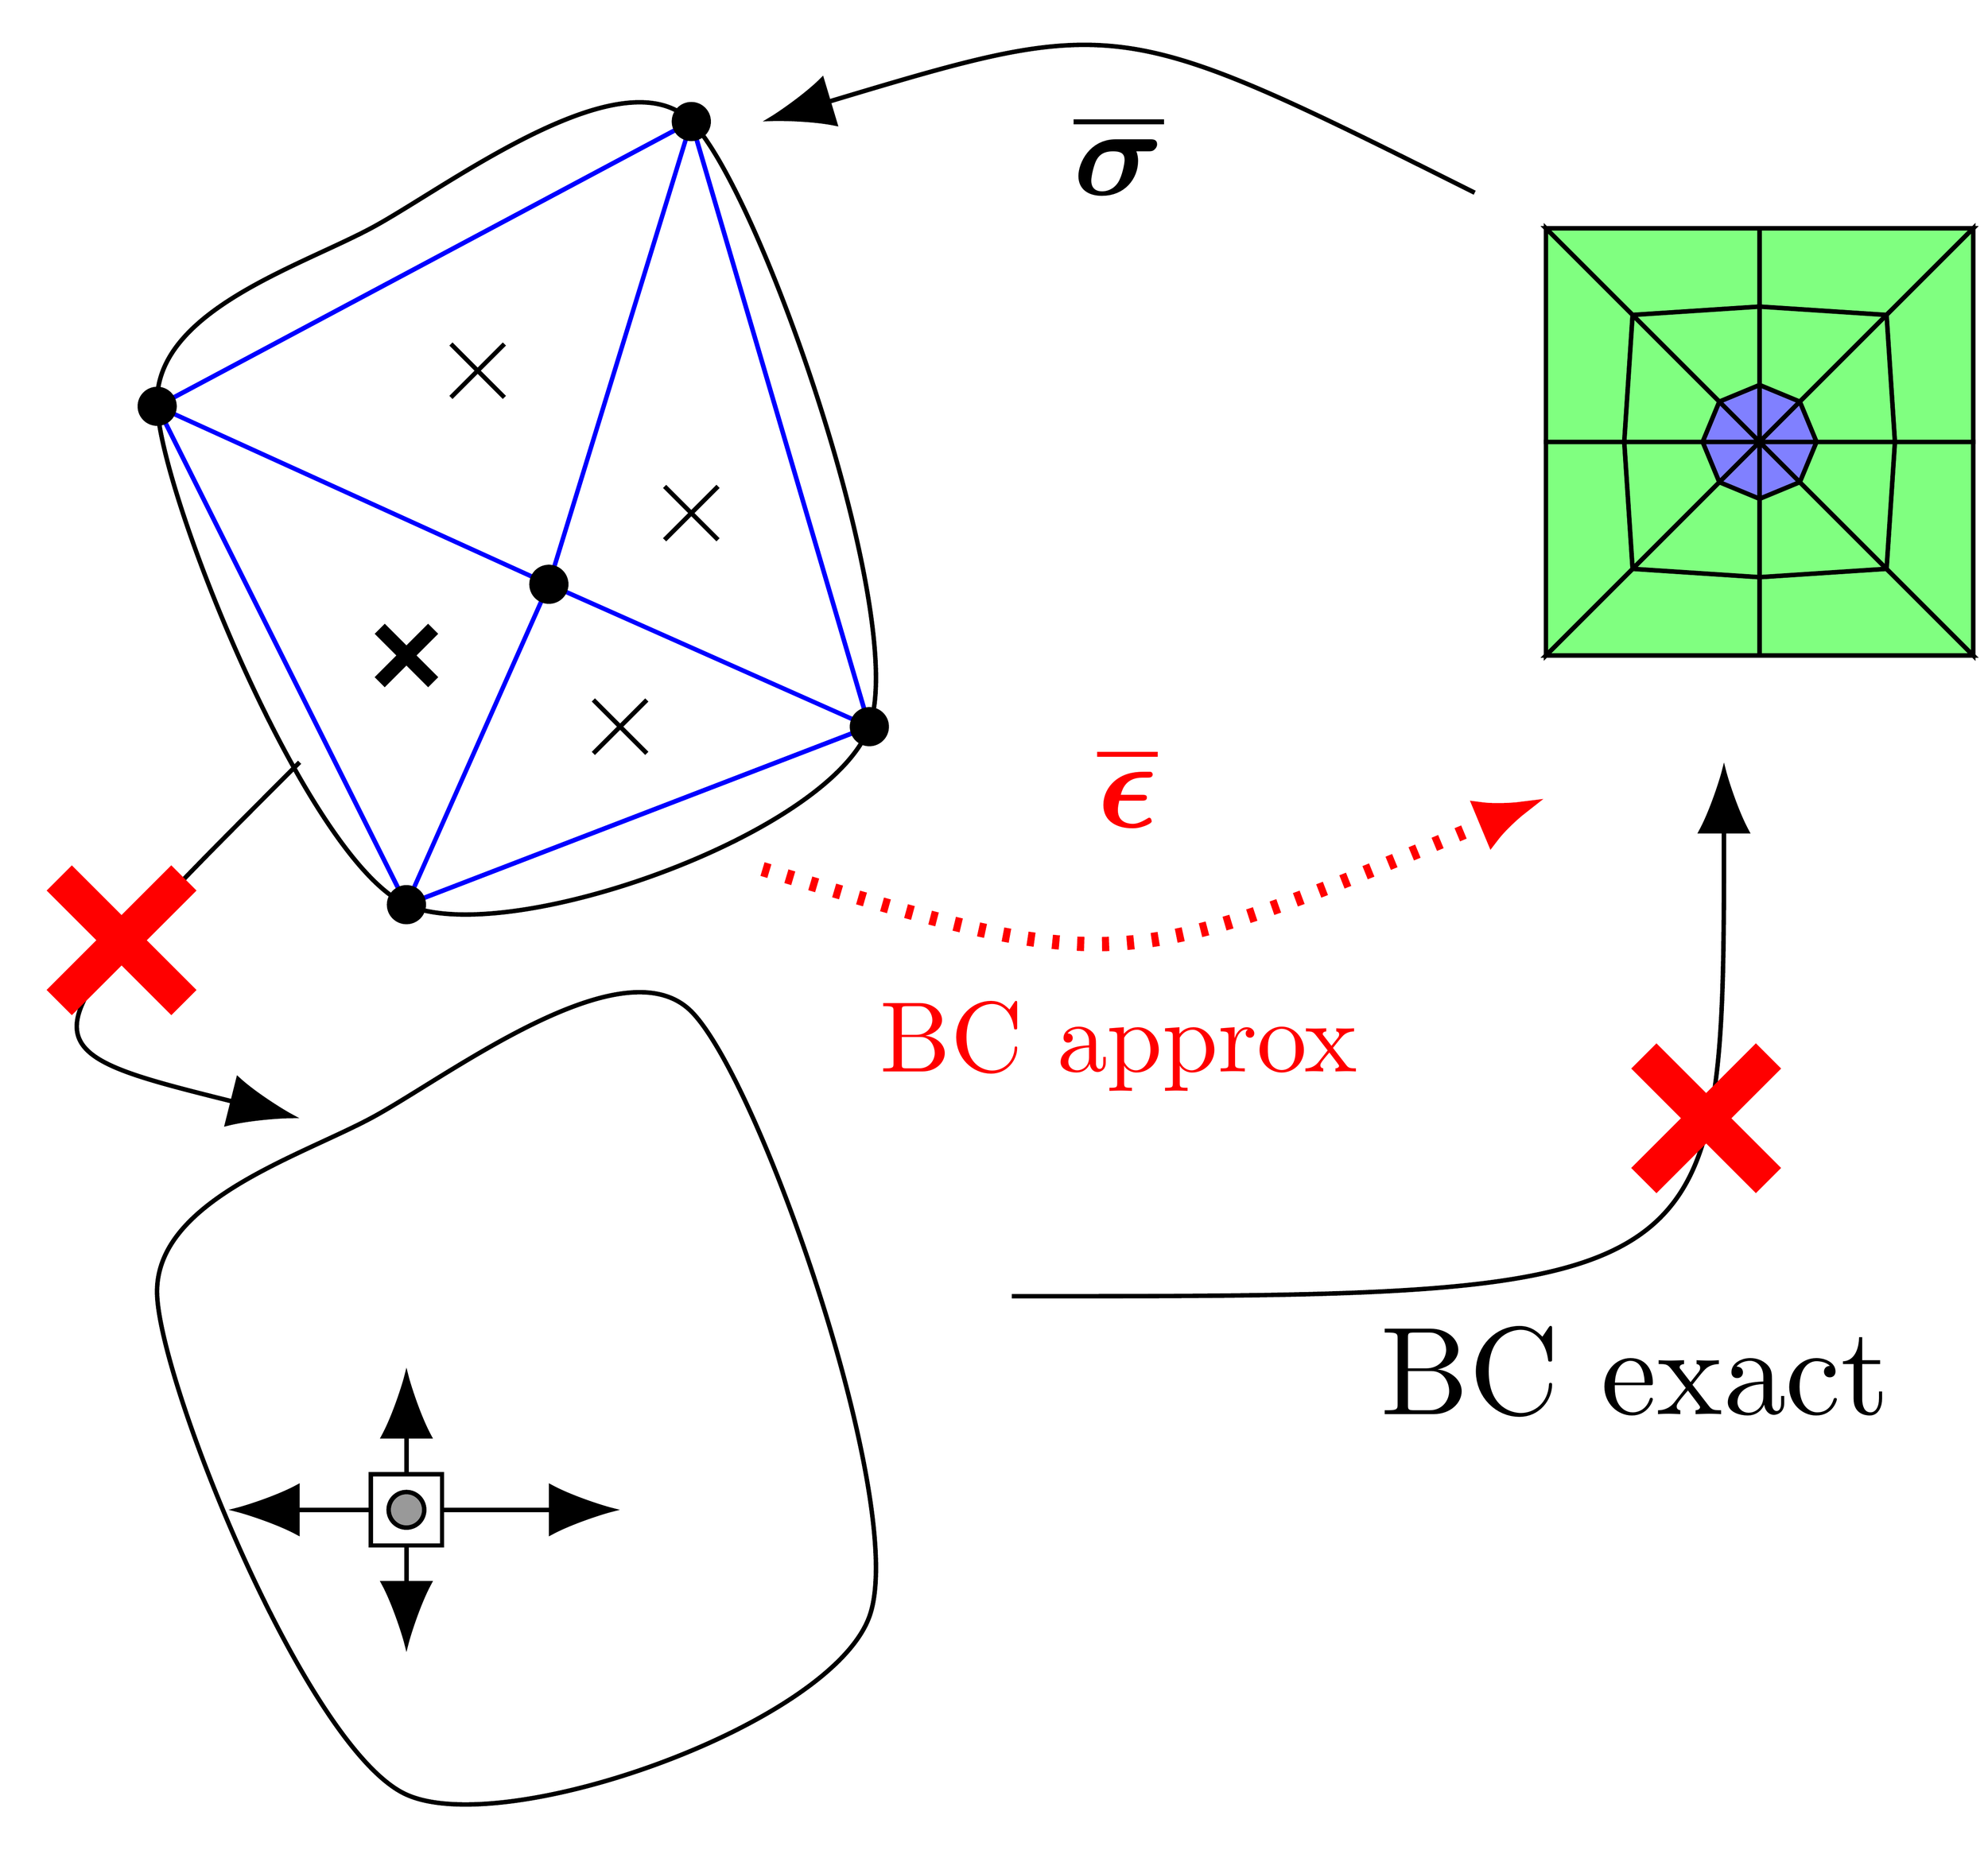
\begin{tikzpicture}[>=latex,node distance=0pt, line width=1.25mm]

% the h.m.s.

    \coordinate [draw=black,shift={(0,0)}] (0) at (6,15);
    \coordinate [draw=black,shift={(0,0)}] (1) at (13,1);
    \coordinate [draw=black,shift={(0,0)}] (2) at (26,6);
    \coordinate [draw=black,shift={(0,0)}] (3) at (21,23);
    \coordinate [draw=black,shift={(0,0)}] (4) at (17,10);
    \draw [blue]  (0) -- (1) -- (2) -- (3) -- cycle;
    \draw [blue]  (0) -- (4);
    \draw [blue]  (1) -- (4);
    \draw [blue]  (2) -- (4);
    \draw [blue]  (3) -- (4);
    \draw [blue]  (6,15) -- (13,1) -- (26,6) -- (21,23) -- cycle;
    \draw [black] plot [smooth cycle] coordinates {(6,15) (13,1) (26,6) (21,23)
    (12,20)};
    \node [fill=black, draw=none, circle, inner sep=0pt, minimum size=1.1cm,scale=1.0] at (0) {};
    \node [fill=black, draw=none, circle, inner sep=0pt, minimum size=1.1cm,scale=1.0] at (1) {};
    \node [fill=black, draw=none, circle, inner sep=0pt, minimum size=1.1cm,scale=1.0] at (2) {};
    \node [fill=black, draw=none, circle, inner sep=0pt, minimum size=1.1cm,scale=1.0] at (3) {};
    \node [fill=black, draw=none, circle, inner sep=0pt, minimum size=1.1cm,scale=1.0] at (4) {};
    \node[cross,minimum size=1.0cm,scale=1.5,line width=0.4cm] (gp_0) at (13,8) {};
    \node[cross,minimum size=1.0cm,scale=1.5] (gp_0) at (15,16) {};
    \node[cross,minimum size=1.0cm,scale=1.5] (gp_0) at (19,6) {};
    \node[cross,minimum size=1.0cm,scale=1.5] (gp_0) at (21,12) {};

% the r.v.e.

    \begin{scope}[yshift = 8 cm,xshift = 45 cm,start chain=going right,scale=4.0]
      \coordinate [draw=black,shift={(0,0)}] (0) at (0,0);
      \coordinate [draw=black,shift={(0,0)}] (1) at (1.5,0);
      \coordinate [draw=black,shift={(0,0)}] (2) at (1.5,1.5);
      \coordinate [draw=black,shift={(0,0)}] (3) at (1.5,1.1);
      \coordinate [draw=black,shift={(0,0)}] (4) at (1.2171572876,1.2171572876);
      \coordinate [draw=black,shift={(0,0)}] (5) at (1.1,1.5);
      \coordinate [draw=black,shift={(0,0)}] (6) at (0,1.5);
      \coordinate [draw=black,shift={(0,0)}] (7) at (0,3);
      \coordinate [draw=black,shift={(0,0)}] (8) at (1.2171572876,1.7828427124);
      \coordinate [draw=black,shift={(0,0)}] (9) at (1.5,1.9);
      \coordinate [draw=black,shift={(0,0)}] (10) at (1.5,3);
      \coordinate [draw=black,shift={(0,0)}] (11) at (3,0);
      \coordinate [draw=black,shift={(0,0)}] (12) at (1.7828427124,1.2171572876);
      \coordinate [draw=black,shift={(0,0)}] (13) at (1.9,1.5);
      \coordinate [draw=black,shift={(0,0)}] (14) at (3,1.5);
      \coordinate [draw=black,shift={(0,0)}] (15) at (3,3);
      \coordinate [draw=black,shift={(0,0)}] (16) at (1.7828427124,1.7828427124);
      \coordinate [draw=black,shift={(0,0)}] (17) at (1.5,0.5500000000014312);
      \coordinate [draw=black,shift={(0,0)}] (18) at (0.6085786437983935,0.6085786437983935);
      \coordinate [draw=black,shift={(0,0)}] (19) at (0.5500000000014312,1.5);
      \coordinate [draw=black,shift={(0,0)}] (20) at (0.6085786437983723,2.391421356201628);
      \coordinate [draw=black,shift={(0,0)}] (21) at (1.5,2.449999999998004);
      \coordinate [draw=black,shift={(0,0)}] (22) at (2.391421356201628,0.6085786437983723);
      \coordinate [draw=black,shift={(0,0)}] (23) at (2.449999999998004,1.5);
      \coordinate [draw=black,shift={(0,0)}] (24) at (2.391421356201648,2.391421356201648);
      \draw [fill=blue!50] (2) --  (4) --  (3) -- cycle;
      \draw [fill=blue!50] (2) --  (4) --  (5) -- cycle;
      \draw [fill=blue!50] (2) --  (8) --  (9) -- cycle;
      \draw [fill=blue!50] (2) --  (8) --  (5) -- cycle;
      \draw [fill=blue!50] (2) --  (12) --  (3) -- cycle;
      \draw [fill=blue!50] (2) --  (12) --  (13) -- cycle;
      \draw [fill=blue!50] (2) --  (16) --  (9) -- cycle;
      \draw [fill=blue!50] (2) --  (16) --  (13) -- cycle;
      \draw [fill=green!50] (0) --  (18) --  (17) --  (1) -- cycle;
      \draw [fill=green!50] (18) --  (4) --  (3) --  (17) -- cycle;
      \draw [fill=green!50] (0) --  (18) --  (19) --  (6) -- cycle;
      \draw [fill=green!50] (18) --  (4) --  (5) --  (19) -- cycle;
      \draw [fill=green!50] (7) --  (20) --  (21) --  (10) -- cycle;
      \draw [fill=green!50] (20) --  (8) --  (9) --  (21) -- cycle;
      \draw [fill=green!50] (7) --  (20) --  (19) --  (6) -- cycle;
      \draw [fill=green!50] (20) --  (8) --  (5) --  (19) -- cycle;
      \draw [fill=green!50] (11) --  (22) --  (17) --  (1) -- cycle;
      \draw [fill=green!50] (22) --  (12) --  (3) --  (17) -- cycle;
      \draw [fill=green!50] (11) --  (22) --  (23) --  (14) -- cycle;
      \draw [fill=green!50] (22) --  (12) --  (13) --  (23) -- cycle;
      \draw [fill=green!50] (15) --  (24) --  (21) --  (10) -- cycle;
      \draw [fill=green!50] (24) --  (16) --  (9) --  (21) -- cycle;
      \draw [fill=green!50] (15) --  (24) --  (23) --  (14) -- cycle;
      \draw [fill=green!50] (24) --  (16) --  (13) --  (23) -- cycle;
      \node [fill=black, draw=none, circle, inner sep=0pt, minimum size=0.1cm,scale=0.3] at (0) {h};
      \node [fill=black, draw=none, circle, inner sep=0pt, minimum size=0.1cm,scale=0.3] at (1) {h};
      \node [fill=black, draw=none, circle, inner sep=0pt, minimum size=0.1cm,scale=0.3] at (2) {h};
      \node [fill=black, draw=none, circle, inner sep=0pt, minimum size=0.1cm,scale=0.3] at (3) {h};
      \node [fill=black, draw=none, circle, inner sep=0pt, minimum size=0.1cm,scale=0.3] at (4) {h};
      \node [fill=black, draw=none, circle, inner sep=0pt, minimum size=0.1cm,scale=0.3] at (5) {h};
      \node [fill=black, draw=none, circle, inner sep=0pt, minimum size=0.1cm,scale=0.3] at (6) {h};
      \node [fill=black, draw=none, circle, inner sep=0pt, minimum size=0.1cm,scale=0.3] at (7) {h};
      \node [fill=black, draw=none, circle, inner sep=0pt, minimum size=0.1cm,scale=0.3] at (8) {h};
      \node [fill=black, draw=none, circle, inner sep=0pt, minimum size=0.1cm,scale=0.3] at (9) {h};
      \node [fill=black, draw=none, circle, inner sep=0pt, minimum size=0.1cm,scale=0.3] at (10) {h};
      \node [fill=black, draw=none, circle, inner sep=0pt, minimum size=0.1cm,scale=0.3] at (11) {h};
      \node [fill=black, draw=none, circle, inner sep=0pt, minimum size=0.1cm,scale=0.3] at (12) {h};
      \node [fill=black, draw=none, circle, inner sep=0pt, minimum size=0.1cm,scale=0.3] at (13) {h};
      \node [fill=black, draw=none, circle, inner sep=0pt, minimum size=0.1cm,scale=0.3] at (14) {h};
      \node [fill=black, draw=none, circle, inner sep=0pt, minimum size=0.1cm,scale=0.3] at (15) {h};
      \node [fill=black, draw=none, circle, inner sep=0pt, minimum size=0.1cm,scale=0.3] at (16) {h};
      \node [fill=black, draw=none, circle, inner sep=0pt, minimum size=0.1cm,scale=0.3] at (17) {h};
      \node [fill=black, draw=none, circle, inner sep=0pt, minimum size=0.1cm,scale=0.3] at (18) {h};
      \node [fill=black, draw=none, circle, inner sep=0pt, minimum size=0.1cm,scale=0.3] at (19) {h};
      \node [fill=black, draw=none, circle, inner sep=0pt, minimum size=0.1cm,scale=0.3] at (20) {h};
      \node [fill=black, draw=none, circle, inner sep=0pt, minimum size=0.1cm,scale=0.3] at (21) {h};
      \node [fill=black, draw=none, circle, inner sep=0pt, minimum size=0.1cm,scale=0.3] at (22) {h};
      \node [fill=black, draw=none, circle, inner sep=0pt, minimum size=0.1cm,scale=0.3] at (23) {h};
      \node [fill=black, draw=none, circle, inner sep=0pt, minimum size=0.1cm,scale=0.3] at (24) {h};
    \end{scope}

    \draw[{Latex[length=20mm,width=15mm]}-] (23,23) ..  controls ++(10,+3) ..
    node[below, scale=10] {$\overline{\bm{\sigma}}$} 
    ++(20,-2);
    \draw[-{Latex[length=20mm,width=15mm]},dashed,dash pattern=on 0.2cm off 0.5cm,red, line width = 0.4cm] (23,2) .. controls ++(10,-3) .. 
    node[above, scale=10] {$\overline{\bm{\epsilon}}$}
    ++(22,+2);
    \node [fill=none, scale=8, red] at (33,-3) {BC approx};

    \draw[-{Latex[length=20mm,width=15mm]}] (10,5) .. controls ++(-8,-8) .. ++(0,-10);
    \draw[-{Latex[length=20mm,width=15mm]}] (30,-10) .. controls ++(20,0) .. node[below=1cm, scale=10] {BC exact}  ++(20,15);
    \node[cross,minimum size=1.0cm,scale=3.5,red,line width=1.0cm] (gp_0) at (5,0) {};
    \node[cross,minimum size=1.0cm,scale=3.5,red,line width=1.0cm] (gp_0) at (49.5,-5) {};

  \begin{scope}[scale=1,xshift = 0cm,yshift = -25cm]
  \draw [black] plot [smooth cycle] coordinates {(6,15) (13,1) (26,6) (21,23) (12,20)};
  \begin{scope}[scale=1,xshift = 4cm,yshift = -2cm]
     \begin{scope}[yshift = 10cm,xshift = 8 cm,start chain=going right]
       \draw (0,0) -- (2,0) -- (2,2) -- (0,2) -- cycle;
       \filldraw[fill=black!40!white,draw=black] (1,1) circle (0.5cm);
       \draw[-{Latex[length=20mm,width=15mm]}] (2,1) -- +(5,0);
       \draw[-{Latex[length=20mm,width=15mm]}] (0,1) -- +(-4,0);
       \draw[-{Latex[length=20mm,width=15mm]}] (1,2) -- +(0,3);
       \draw[-{Latex[length=20mm,width=15mm]}] (1,0) -- +(0,-3);
     \end{scope}
  \end{scope}
  \end{scope}

  \end{tikzpicture}

\end{document}
}
\end{figure}
\end{frame}

%------------------------------------------------

\begin{frame}
\frametitle{Boundary conditions}

\begin{minipage}[h]{0.49\linewidth}
\begin{itemize}
\item Uniform Strain: \\ $\bm{u} = \overline{\bm{\epsilon}} \cdot \bm{x} $
  \vspace{0.5cm}
\item Uniform Stress: \\$ \bm{\sigma} = \overline{\bm{\sigma}} $
  \vspace{0.5cm}
\item Periodic \\
$ \bm{u}^+ - \bm{u}^- = \overline{\bm{\epsilon}} \cdot (\bm{x}^+ - \bm{x}^-) $\\
$ \bm{\sigma}^+ \cdot \hat{n}  = \bm{\sigma}^- \cdot \hat{n}$
\end{itemize}
\end{minipage}
\begin{minipage}[h]{0.49\linewidth}
\resizebox{0.8\linewidth}{!}{\documentclass{standalone}

\begin{document}

\tikzset{cross/.style={cross out, draw=black, fill=none, minimum size=2*(#1-\pgflinewidth), inner sep=0pt, outer
sep=0pt}, cross/.default={2pt}}

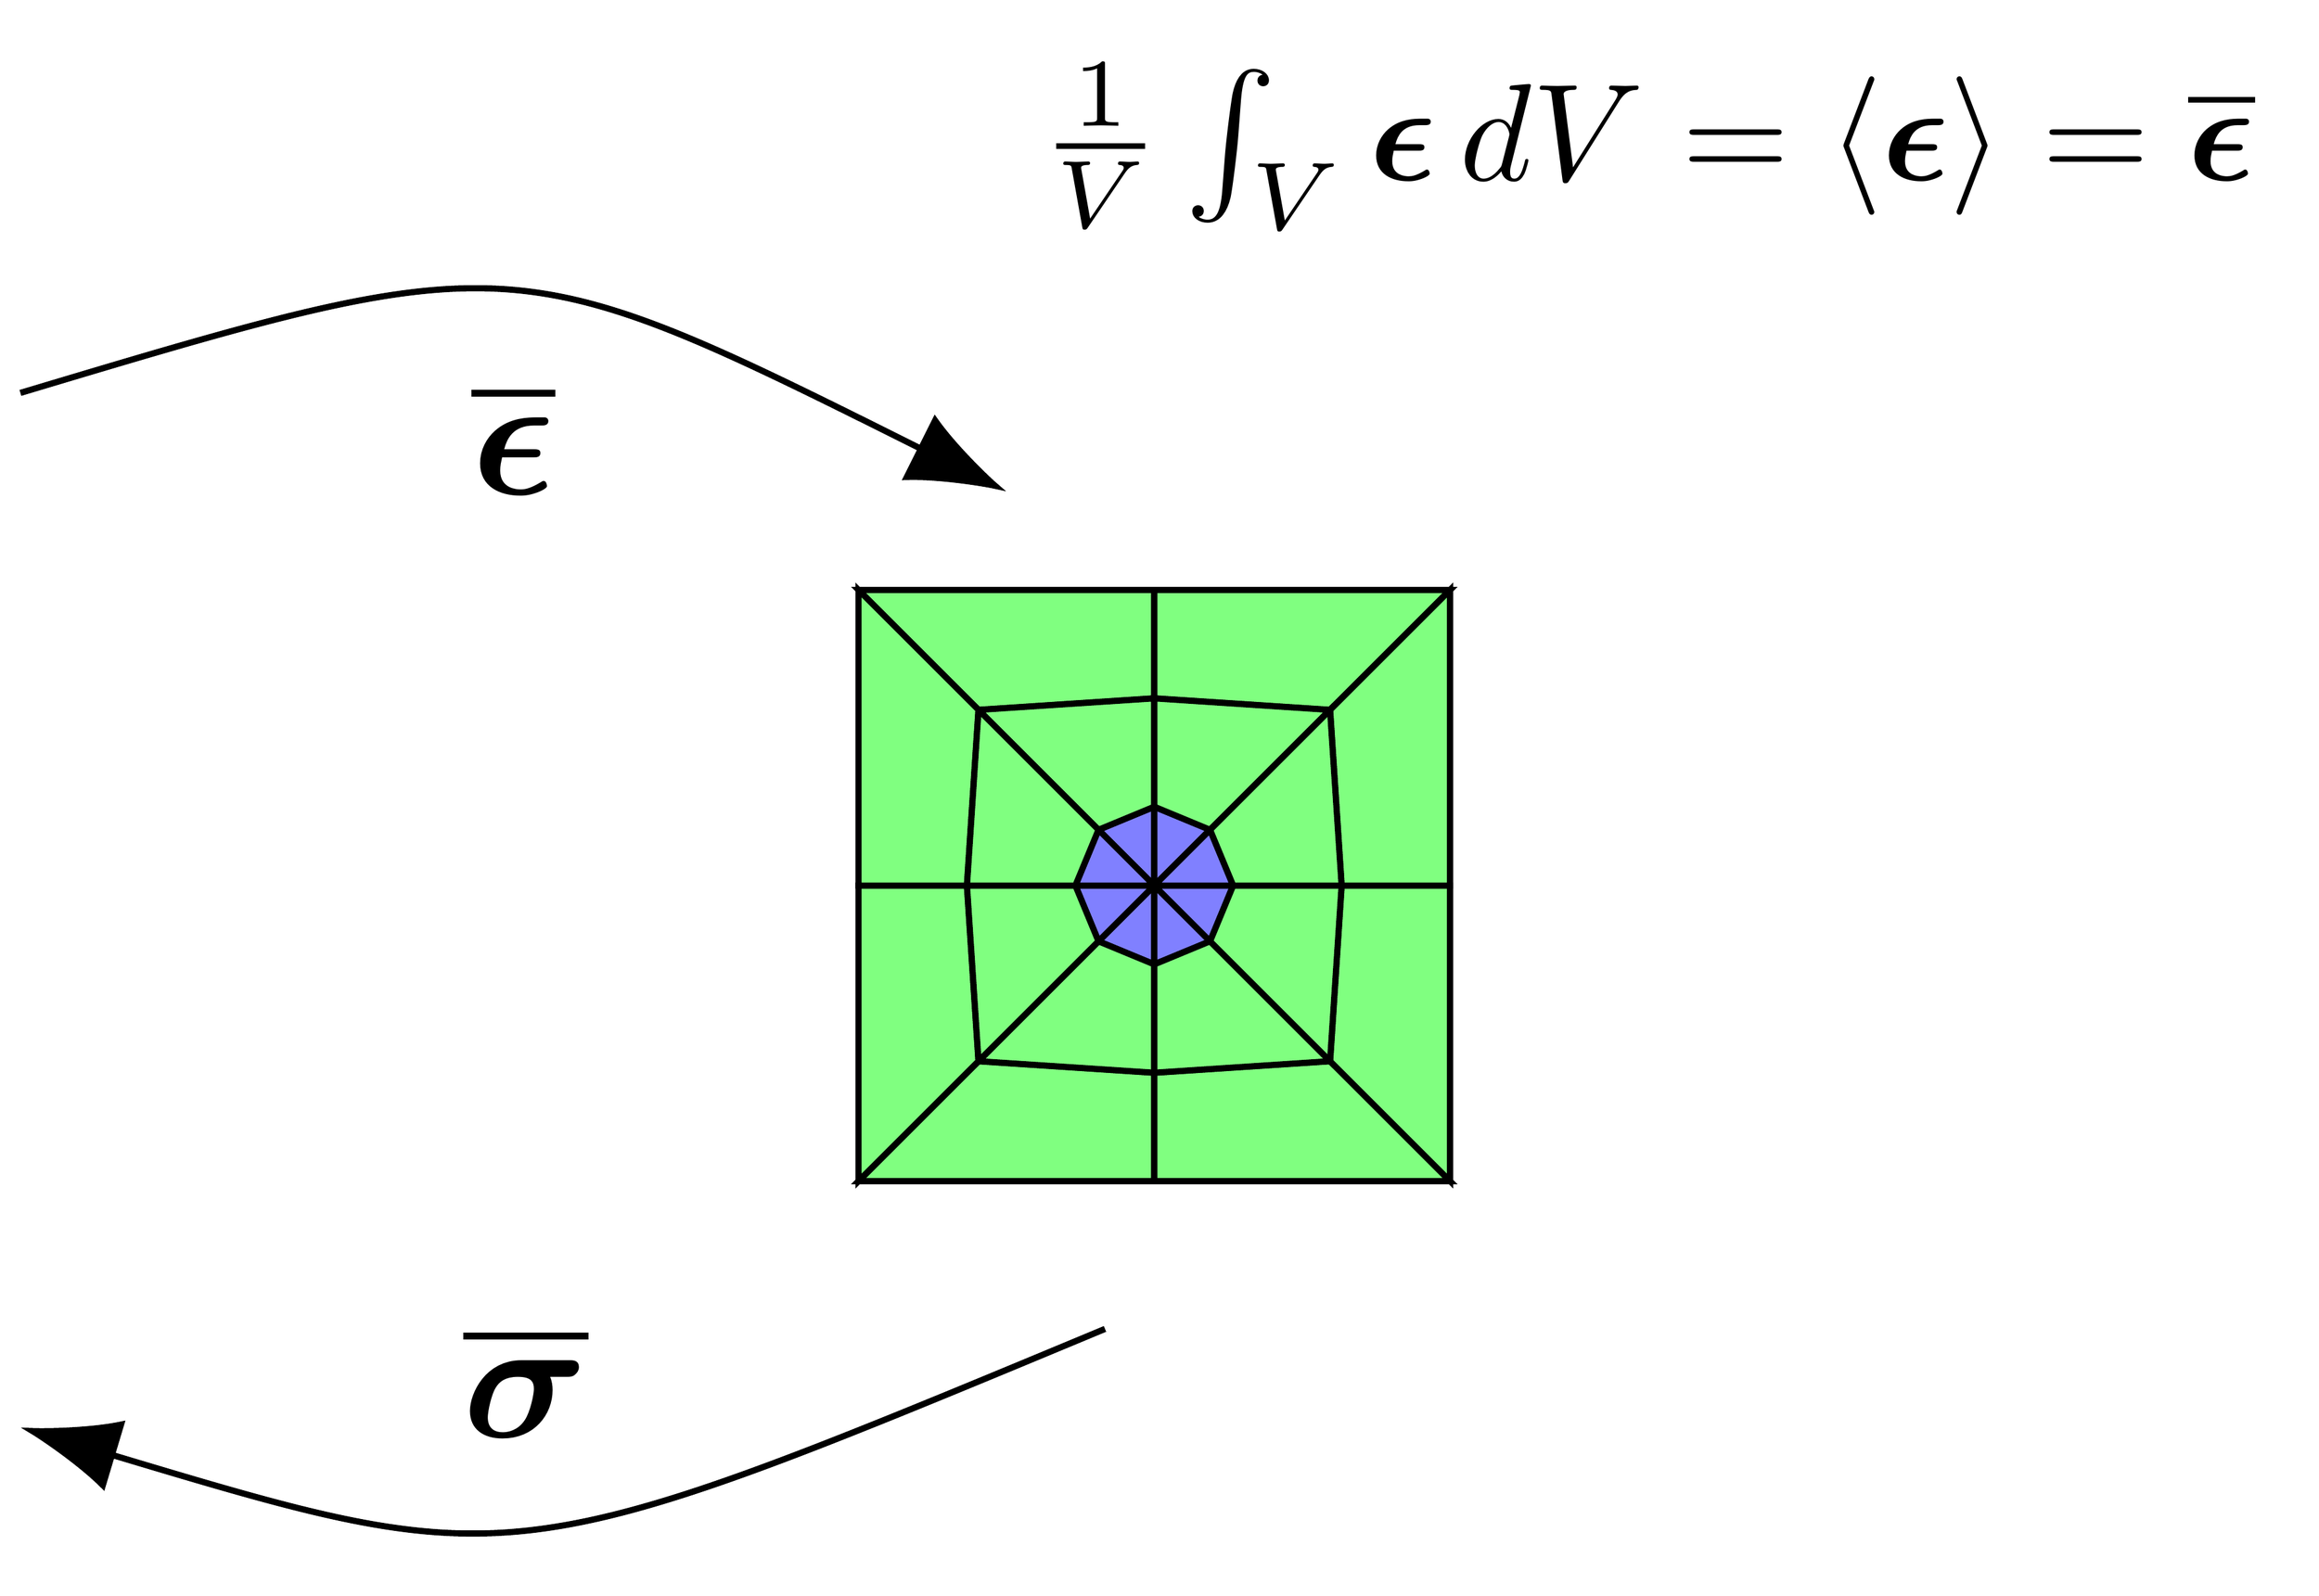
\begin{tikzpicture}[>=latex,node distance=0pt, line width=1.25mm]

    \begin{scope}[yshift=7 cm, xshift=40cm, start chain=going right, scale=4.0]
      \coordinate [draw=black,shift={(0,0)}] (0) at (0,0);
      \coordinate [draw=black,shift={(0,0)}] (1) at (1.5,0);
      \coordinate [draw=black,shift={(0,0)}] (2) at (1.5,1.5);
      \coordinate [draw=black,shift={(0,0)}] (3) at (1.5,1.1);
      \coordinate [draw=black,shift={(0,0)}] (4) at (1.2171572876,1.2171572876);
      \coordinate [draw=black,shift={(0,0)}] (5) at (1.1,1.5);
      \coordinate [draw=black,shift={(0,0)}] (6) at (0,1.5);
      \coordinate [draw=black,shift={(0,0)}] (7) at (0,3);
      \coordinate [draw=black,shift={(0,0)}] (8) at (1.2171572876,1.7828427124);
      \coordinate [draw=black,shift={(0,0)}] (9) at (1.5,1.9);
      \coordinate [draw=black,shift={(0,0)}] (10) at (1.5,3);
      \coordinate [draw=black,shift={(0,0)}] (11) at (3,0);
      \coordinate [draw=black,shift={(0,0)}] (12) at (1.7828427124,1.2171572876);
      \coordinate [draw=black,shift={(0,0)}] (13) at (1.9,1.5);
      \coordinate [draw=black,shift={(0,0)}] (14) at (3,1.5);
      \coordinate [draw=black,shift={(0,0)}] (15) at (3,3);
      \coordinate [draw=black,shift={(0,0)}] (16) at (1.7828427124,1.7828427124);
      \coordinate [draw=black,shift={(0,0)}] (17) at (1.5,0.5500000000014312);
      \coordinate [draw=black,shift={(0,0)}] (18) at (0.6085786437983935,0.6085786437983935);
      \coordinate [draw=black,shift={(0,0)}] (19) at (0.5500000000014312,1.5);
      \coordinate [draw=black,shift={(0,0)}] (20) at (0.6085786437983723,2.391421356201628);
      \coordinate [draw=black,shift={(0,0)}] (21) at (1.5,2.449999999998004);
      \coordinate [draw=black,shift={(0,0)}] (22) at (2.391421356201628,0.6085786437983723);
      \coordinate [draw=black,shift={(0,0)}] (23) at (2.449999999998004,1.5);
      \coordinate [draw=black,shift={(0,0)}] (24) at (2.391421356201648,2.391421356201648);
      \draw [fill=blue!50] (2) --  (4) --  (3) -- cycle;
      \draw [fill=blue!50] (2) --  (4) --  (5) -- cycle;
      \draw [fill=blue!50] (2) --  (8) --  (9) -- cycle;
      \draw [fill=blue!50] (2) --  (8) --  (5) -- cycle;
      \draw [fill=blue!50] (2) --  (12) --  (3) -- cycle;
      \draw [fill=blue!50] (2) --  (12) --  (13) -- cycle;
      \draw [fill=blue!50] (2) --  (16) --  (9) -- cycle;
      \draw [fill=blue!50] (2) --  (16) --  (13) -- cycle;
      \draw [fill=green!50] (0) --  (18) --  (17) --  (1) -- cycle;
      \draw [fill=green!50] (18) --  (4) --  (3) --  (17) -- cycle;
      \draw [fill=green!50] (0) --  (18) --  (19) --  (6) -- cycle;
      \draw [fill=green!50] (18) --  (4) --  (5) --  (19) -- cycle;
      \draw [fill=green!50] (7) --  (20) --  (21) --  (10) -- cycle;
      \draw [fill=green!50] (20) --  (8) --  (9) --  (21) -- cycle;
      \draw [fill=green!50] (7) --  (20) --  (19) --  (6) -- cycle;
      \draw [fill=green!50] (20) --  (8) --  (5) --  (19) -- cycle;
      \draw [fill=green!50] (11) --  (22) --  (17) --  (1) -- cycle;
      \draw [fill=green!50] (22) --  (12) --  (3) --  (17) -- cycle;
      \draw [fill=green!50] (11) --  (22) --  (23) --  (14) -- cycle;
      \draw [fill=green!50] (22) --  (12) --  (13) --  (23) -- cycle;
      \draw [fill=green!50] (15) --  (24) --  (21) --  (10) -- cycle;
      \draw [fill=green!50] (24) --  (16) --  (9) --  (21) -- cycle;
      \draw [fill=green!50] (15) --  (24) --  (23) --  (14) -- cycle;
      \draw [fill=green!50] (24) --  (16) --  (13) --  (23) -- cycle;
      \node [fill=black, draw=none, circle, inner sep=0pt, minimum size=0.1cm,scale=0.3] at (0) {h};
      \node [fill=black, draw=none, circle, inner sep=0pt, minimum size=0.1cm,scale=0.3] at (1) {h};
      \node [fill=black, draw=none, circle, inner sep=0pt, minimum size=0.1cm,scale=0.3] at (2) {h};
      \node [fill=black, draw=none, circle, inner sep=0pt, minimum size=0.1cm,scale=0.3] at (3) {h};
      \node [fill=black, draw=none, circle, inner sep=0pt, minimum size=0.1cm,scale=0.3] at (4) {h};
      \node [fill=black, draw=none, circle, inner sep=0pt, minimum size=0.1cm,scale=0.3] at (5) {h};
      \node [fill=black, draw=none, circle, inner sep=0pt, minimum size=0.1cm,scale=0.3] at (6) {h};
      \node [fill=black, draw=none, circle, inner sep=0pt, minimum size=0.1cm,scale=0.3] at (7) {h};
      \node [fill=black, draw=none, circle, inner sep=0pt, minimum size=0.1cm,scale=0.3] at (8) {h};
      \node [fill=black, draw=none, circle, inner sep=0pt, minimum size=0.1cm,scale=0.3] at (9) {h};
      \node [fill=black, draw=none, circle, inner sep=0pt, minimum size=0.1cm,scale=0.3] at (10) {h};
      \node [fill=black, draw=none, circle, inner sep=0pt, minimum size=0.1cm,scale=0.3] at (11) {h};
      \node [fill=black, draw=none, circle, inner sep=0pt, minimum size=0.1cm,scale=0.3] at (12) {h};
      \node [fill=black, draw=none, circle, inner sep=0pt, minimum size=0.1cm,scale=0.3] at (13) {h};
      \node [fill=black, draw=none, circle, inner sep=0pt, minimum size=0.1cm,scale=0.3] at (14) {h};
      \node [fill=black, draw=none, circle, inner sep=0pt, minimum size=0.1cm,scale=0.3] at (15) {h};
      \node [fill=black, draw=none, circle, inner sep=0pt, minimum size=0.1cm,scale=0.3] at (16) {h};
      \node [fill=black, draw=none, circle, inner sep=0pt, minimum size=0.1cm,scale=0.3] at (17) {h};
      \node [fill=black, draw=none, circle, inner sep=0pt, minimum size=0.1cm,scale=0.3] at (18) {h};
      \node [fill=black, draw=none, circle, inner sep=0pt, minimum size=0.1cm,scale=0.3] at (19) {h};
      \node [fill=black, draw=none, circle, inner sep=0pt, minimum size=0.1cm,scale=0.3] at (20) {h};
      \node [fill=black, draw=none, circle, inner sep=0pt, minimum size=0.1cm,scale=0.3] at (21) {h};
      \node [fill=black, draw=none, circle, inner sep=0pt, minimum size=0.1cm,scale=0.3] at (22) {h};
      \node [fill=black, draw=none, circle, inner sep=0pt, minimum size=0.1cm,scale=0.3] at (23) {h};
      \node [fill=black, draw=none, circle, inner sep=0pt, minimum size=0.1cm,scale=0.3] at (24) {h};
    \end{scope}

    \draw[-{Latex[length=20mm,width=15mm]}] (23,23) ..  controls ++(10,+3) ..
    node[below, scale=10] {$\overline{\bm{\epsilon}}$} 
    ++(20,-2);
    \draw[{Latex[length=20mm,width=15mm]}-] (23,2) .. controls ++(10,-3) .. 
    node[above, scale=10] {$\overline{\bm{\sigma}}$}
    ++(22,+2);

    \node[scale=8] at (56,28) {$\frac{1}{V} \int_{V} \bm{\epsilon} \, dV = \langle \bm{\epsilon} \rangle = \overline{\bm{\epsilon}}$} ;

\end{tikzpicture}

\end{document}

}
\end{minipage}

\end{frame}

%------------------------------------------------

\begin{frame}
\frametitle{Boundary conditions}

\begin{minipage}[h]{0.49\linewidth}
\begin{itemize}
\item Uniform Strain: \\ $\bm{u} = \overline{\bm{\epsilon}} \cdot \bm{x} $
  \begin{itemize}
  \item Dirichlet
  \end{itemize}
  \vspace{0.5cm}
\item Uniform Stress: \\$ \bm{\sigma} = \overline{\bm{\sigma}} $
  \begin{itemize}
  \item Lagrange multipliers
  \end{itemize}
  \vspace{0.5cm}
\item Periodic \\
$ \bm{u}^+ - \bm{u}^- = \overline{\bm{\epsilon}} \cdot (\bm{x}^+ - \bm{x}^-) $\\
$ \bm{\sigma}^+ \cdot \hat{n}  = \bm{\sigma}^- \cdot \hat{n}$
  \begin{itemize}
  \item Lagrange multipliers
  \item Unknowns elimination
  \end{itemize}
\end{itemize}
\end{minipage}
\begin{minipage}[h]{0.49\linewidth}
\resizebox{0.8\linewidth}{!}{\documentclass{standalone}

\begin{document}

\tikzset{cross/.style={cross out, draw=black, fill=none, minimum size=2*(#1-\pgflinewidth), inner sep=0pt, outer
sep=0pt}, cross/.default={2pt}}

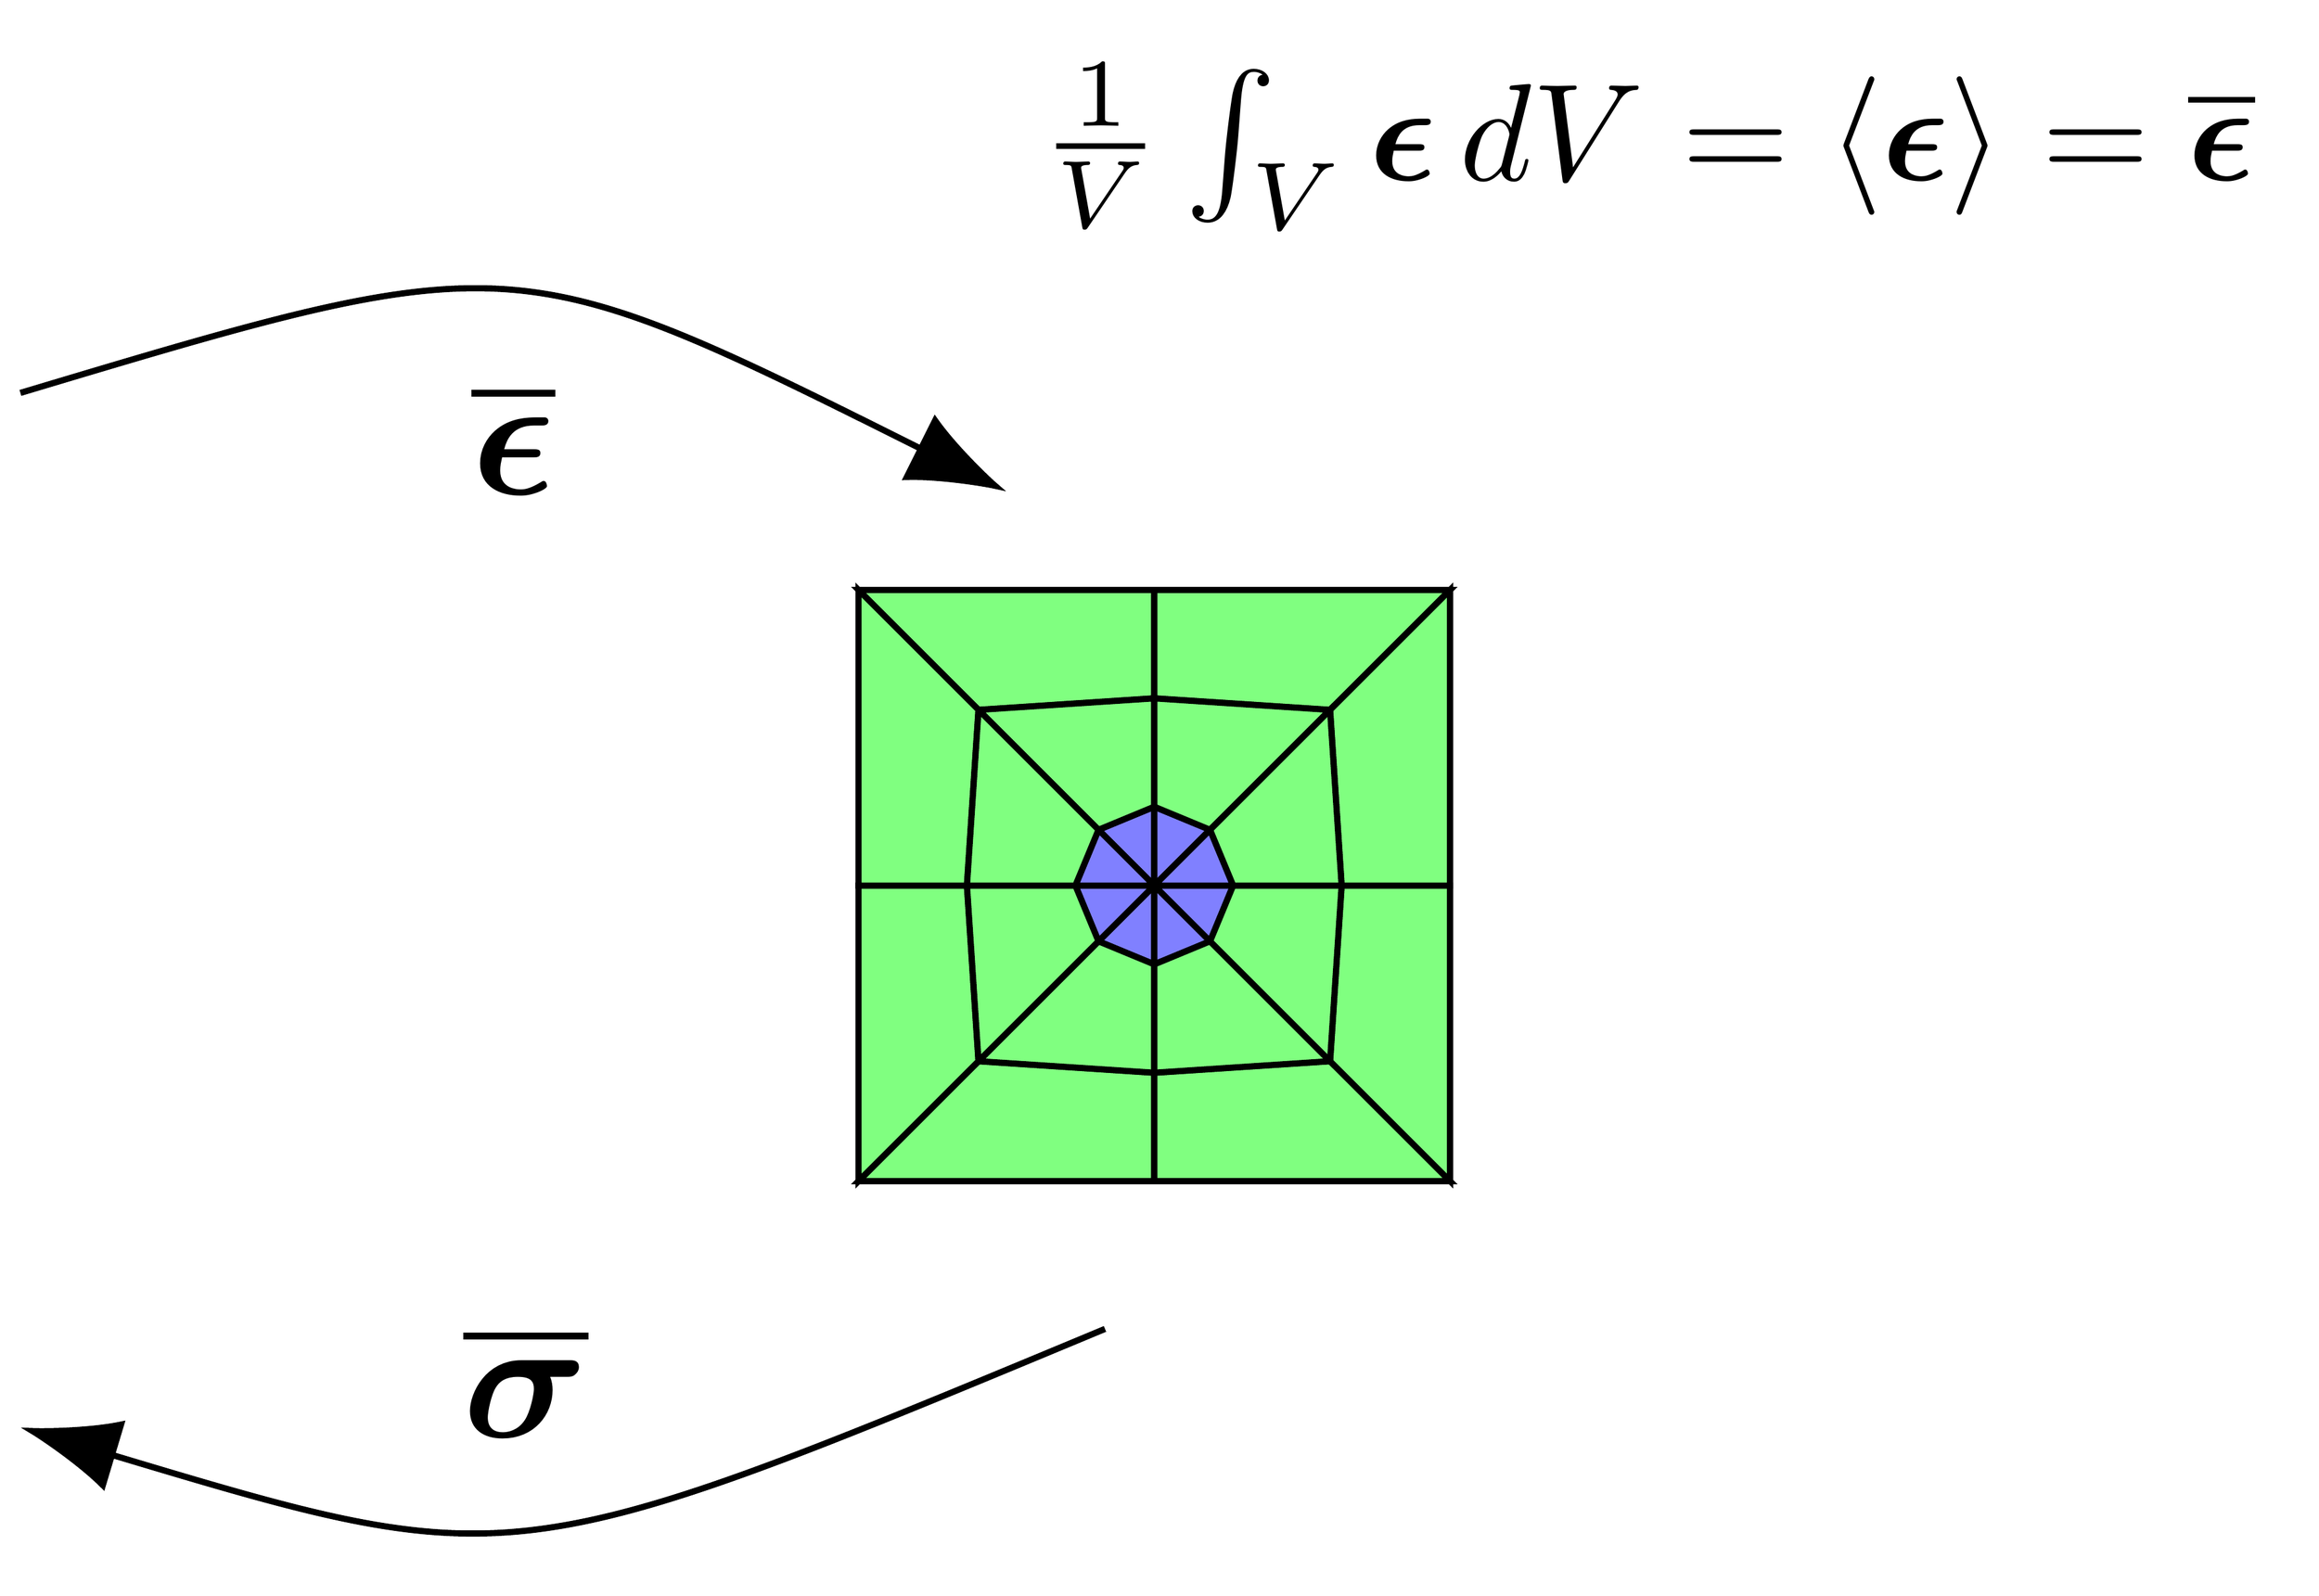
\begin{tikzpicture}[>=latex,node distance=0pt, line width=1.25mm]

    \begin{scope}[yshift=7 cm, xshift=40cm, start chain=going right, scale=4.0]
      \coordinate [draw=black,shift={(0,0)}] (0) at (0,0);
      \coordinate [draw=black,shift={(0,0)}] (1) at (1.5,0);
      \coordinate [draw=black,shift={(0,0)}] (2) at (1.5,1.5);
      \coordinate [draw=black,shift={(0,0)}] (3) at (1.5,1.1);
      \coordinate [draw=black,shift={(0,0)}] (4) at (1.2171572876,1.2171572876);
      \coordinate [draw=black,shift={(0,0)}] (5) at (1.1,1.5);
      \coordinate [draw=black,shift={(0,0)}] (6) at (0,1.5);
      \coordinate [draw=black,shift={(0,0)}] (7) at (0,3);
      \coordinate [draw=black,shift={(0,0)}] (8) at (1.2171572876,1.7828427124);
      \coordinate [draw=black,shift={(0,0)}] (9) at (1.5,1.9);
      \coordinate [draw=black,shift={(0,0)}] (10) at (1.5,3);
      \coordinate [draw=black,shift={(0,0)}] (11) at (3,0);
      \coordinate [draw=black,shift={(0,0)}] (12) at (1.7828427124,1.2171572876);
      \coordinate [draw=black,shift={(0,0)}] (13) at (1.9,1.5);
      \coordinate [draw=black,shift={(0,0)}] (14) at (3,1.5);
      \coordinate [draw=black,shift={(0,0)}] (15) at (3,3);
      \coordinate [draw=black,shift={(0,0)}] (16) at (1.7828427124,1.7828427124);
      \coordinate [draw=black,shift={(0,0)}] (17) at (1.5,0.5500000000014312);
      \coordinate [draw=black,shift={(0,0)}] (18) at (0.6085786437983935,0.6085786437983935);
      \coordinate [draw=black,shift={(0,0)}] (19) at (0.5500000000014312,1.5);
      \coordinate [draw=black,shift={(0,0)}] (20) at (0.6085786437983723,2.391421356201628);
      \coordinate [draw=black,shift={(0,0)}] (21) at (1.5,2.449999999998004);
      \coordinate [draw=black,shift={(0,0)}] (22) at (2.391421356201628,0.6085786437983723);
      \coordinate [draw=black,shift={(0,0)}] (23) at (2.449999999998004,1.5);
      \coordinate [draw=black,shift={(0,0)}] (24) at (2.391421356201648,2.391421356201648);
      \draw [fill=blue!50] (2) --  (4) --  (3) -- cycle;
      \draw [fill=blue!50] (2) --  (4) --  (5) -- cycle;
      \draw [fill=blue!50] (2) --  (8) --  (9) -- cycle;
      \draw [fill=blue!50] (2) --  (8) --  (5) -- cycle;
      \draw [fill=blue!50] (2) --  (12) --  (3) -- cycle;
      \draw [fill=blue!50] (2) --  (12) --  (13) -- cycle;
      \draw [fill=blue!50] (2) --  (16) --  (9) -- cycle;
      \draw [fill=blue!50] (2) --  (16) --  (13) -- cycle;
      \draw [fill=green!50] (0) --  (18) --  (17) --  (1) -- cycle;
      \draw [fill=green!50] (18) --  (4) --  (3) --  (17) -- cycle;
      \draw [fill=green!50] (0) --  (18) --  (19) --  (6) -- cycle;
      \draw [fill=green!50] (18) --  (4) --  (5) --  (19) -- cycle;
      \draw [fill=green!50] (7) --  (20) --  (21) --  (10) -- cycle;
      \draw [fill=green!50] (20) --  (8) --  (9) --  (21) -- cycle;
      \draw [fill=green!50] (7) --  (20) --  (19) --  (6) -- cycle;
      \draw [fill=green!50] (20) --  (8) --  (5) --  (19) -- cycle;
      \draw [fill=green!50] (11) --  (22) --  (17) --  (1) -- cycle;
      \draw [fill=green!50] (22) --  (12) --  (3) --  (17) -- cycle;
      \draw [fill=green!50] (11) --  (22) --  (23) --  (14) -- cycle;
      \draw [fill=green!50] (22) --  (12) --  (13) --  (23) -- cycle;
      \draw [fill=green!50] (15) --  (24) --  (21) --  (10) -- cycle;
      \draw [fill=green!50] (24) --  (16) --  (9) --  (21) -- cycle;
      \draw [fill=green!50] (15) --  (24) --  (23) --  (14) -- cycle;
      \draw [fill=green!50] (24) --  (16) --  (13) --  (23) -- cycle;
      \node [fill=black, draw=none, circle, inner sep=0pt, minimum size=0.1cm,scale=0.3] at (0) {h};
      \node [fill=black, draw=none, circle, inner sep=0pt, minimum size=0.1cm,scale=0.3] at (1) {h};
      \node [fill=black, draw=none, circle, inner sep=0pt, minimum size=0.1cm,scale=0.3] at (2) {h};
      \node [fill=black, draw=none, circle, inner sep=0pt, minimum size=0.1cm,scale=0.3] at (3) {h};
      \node [fill=black, draw=none, circle, inner sep=0pt, minimum size=0.1cm,scale=0.3] at (4) {h};
      \node [fill=black, draw=none, circle, inner sep=0pt, minimum size=0.1cm,scale=0.3] at (5) {h};
      \node [fill=black, draw=none, circle, inner sep=0pt, minimum size=0.1cm,scale=0.3] at (6) {h};
      \node [fill=black, draw=none, circle, inner sep=0pt, minimum size=0.1cm,scale=0.3] at (7) {h};
      \node [fill=black, draw=none, circle, inner sep=0pt, minimum size=0.1cm,scale=0.3] at (8) {h};
      \node [fill=black, draw=none, circle, inner sep=0pt, minimum size=0.1cm,scale=0.3] at (9) {h};
      \node [fill=black, draw=none, circle, inner sep=0pt, minimum size=0.1cm,scale=0.3] at (10) {h};
      \node [fill=black, draw=none, circle, inner sep=0pt, minimum size=0.1cm,scale=0.3] at (11) {h};
      \node [fill=black, draw=none, circle, inner sep=0pt, minimum size=0.1cm,scale=0.3] at (12) {h};
      \node [fill=black, draw=none, circle, inner sep=0pt, minimum size=0.1cm,scale=0.3] at (13) {h};
      \node [fill=black, draw=none, circle, inner sep=0pt, minimum size=0.1cm,scale=0.3] at (14) {h};
      \node [fill=black, draw=none, circle, inner sep=0pt, minimum size=0.1cm,scale=0.3] at (15) {h};
      \node [fill=black, draw=none, circle, inner sep=0pt, minimum size=0.1cm,scale=0.3] at (16) {h};
      \node [fill=black, draw=none, circle, inner sep=0pt, minimum size=0.1cm,scale=0.3] at (17) {h};
      \node [fill=black, draw=none, circle, inner sep=0pt, minimum size=0.1cm,scale=0.3] at (18) {h};
      \node [fill=black, draw=none, circle, inner sep=0pt, minimum size=0.1cm,scale=0.3] at (19) {h};
      \node [fill=black, draw=none, circle, inner sep=0pt, minimum size=0.1cm,scale=0.3] at (20) {h};
      \node [fill=black, draw=none, circle, inner sep=0pt, minimum size=0.1cm,scale=0.3] at (21) {h};
      \node [fill=black, draw=none, circle, inner sep=0pt, minimum size=0.1cm,scale=0.3] at (22) {h};
      \node [fill=black, draw=none, circle, inner sep=0pt, minimum size=0.1cm,scale=0.3] at (23) {h};
      \node [fill=black, draw=none, circle, inner sep=0pt, minimum size=0.1cm,scale=0.3] at (24) {h};
    \end{scope}

    \draw[-{Latex[length=20mm,width=15mm]}] (23,23) ..  controls ++(10,+3) ..
    node[below, scale=10] {$\overline{\bm{\epsilon}}$} 
    ++(20,-2);
    \draw[{Latex[length=20mm,width=15mm]}-] (23,2) .. controls ++(10,-3) .. 
    node[above, scale=10] {$\overline{\bm{\sigma}}$}
    ++(22,+2);

    \node[scale=8] at (56,28) {$\frac{1}{V} \int_{V} \bm{\epsilon} \, dV = \langle \bm{\epsilon} \rangle = \overline{\bm{\epsilon}}$} ;

\end{tikzpicture}

\end{document}

}
\end{minipage}

\end{frame}

%------------------------------------------------

\begin{frame}
\frametitle{Boundary conditions}

\begin{minipage}[h]{0.49\linewidth}
\begin{itemize}
\item Uniform Strain: \\ $\bm{u} = \overline{\bm{\epsilon}} \cdot \bm{x} $
  \begin{itemize}
  \item Dirichlet
  \end{itemize}
  \vspace{0.5cm}
\item Uniform Stress: \\$ \bm{\sigma} = \overline{\bm{\sigma}} $
  \begin{itemize}
  \item Lagrange multipliers
  \end{itemize}
  \vspace{0.5cm}
\item Periodic \\
$ \bm{u}^+ - \bm{u}^- = \overline{\bm{\epsilon}} \cdot (\bm{x}^+ - \bm{x}^-) $\\
$ \bm{\sigma}^+ \cdot \hat{n}  = \bm{\sigma}^- \cdot \hat{n}$
  \begin{itemize}
  \item Lagrange multipliers
  \item Unknowns elimination
  \end{itemize}
\end{itemize}
\end{minipage}
\begin{minipage}[h]{0.49\linewidth}
\resizebox{1.1\linewidth}{!}{
\begin{tikzpicture}[node distance=4cm]
    \node[inner sep=0pt, scale=0.1] (rve) at (0,2) {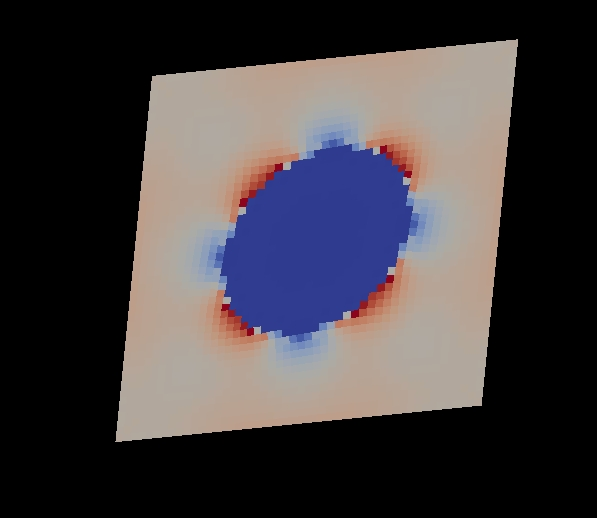
\includegraphics[width=1.4\textwidth]{figures/unif_strain_exy.jpg}};
    \node[inner sep=0pt, scale=0.1] (rve) at (0,1) {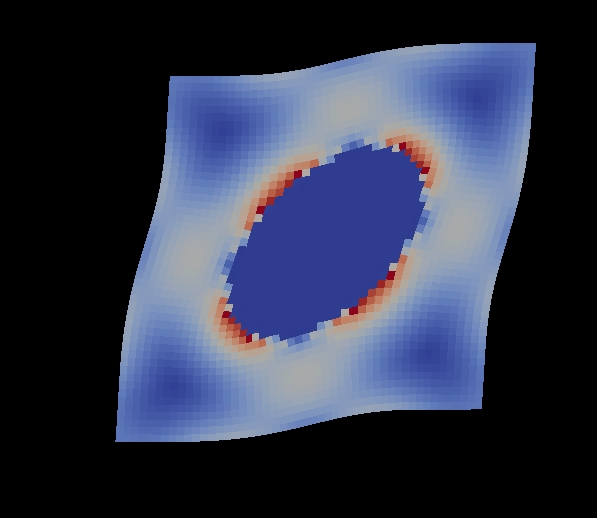
\includegraphics[width=1.4\textwidth]{figures/unif_stress_exy.jpg}};
    \node[inner sep=0pt, scale=0.1] (rve) at (0,0) {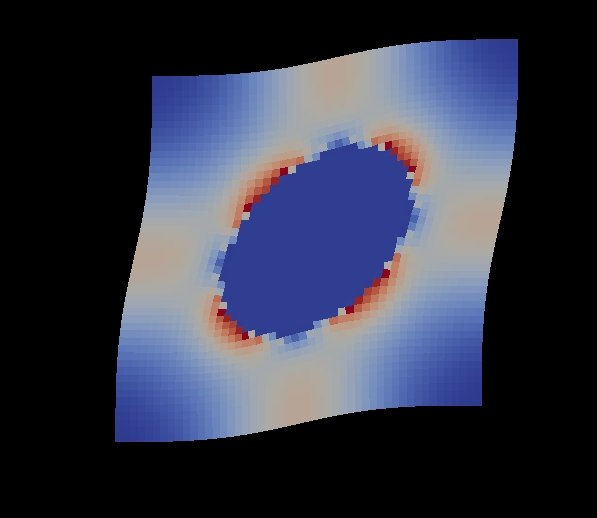
\includegraphics[width=1.4\textwidth]{figures/periodic_exy.jpg}};
    \node[inner sep=0pt, scale=0.6] (rve) at (1.1,1) {$\overline{\bm{\epsilon}} = \begin{bmatrix} 0 \\0 \\ \epsilon_{xy}\end{bmatrix}$};
\end{tikzpicture}
}
\end{minipage}

\end{frame}

%------------------------------------------------

\begin{frame}
\frametitle{The FE$^2$ multi-scale method}

\begin{figure}[!ht]
\resizebox{1.0\linewidth}{!}{\documentclass{standalone}

\begin{document}

\tikzset{cross/.style={cross out, draw=black, fill=none, minimum size=2*(#1-\pgflinewidth), inner sep=0pt, outer
sep=0pt}, cross/.default={2pt}}

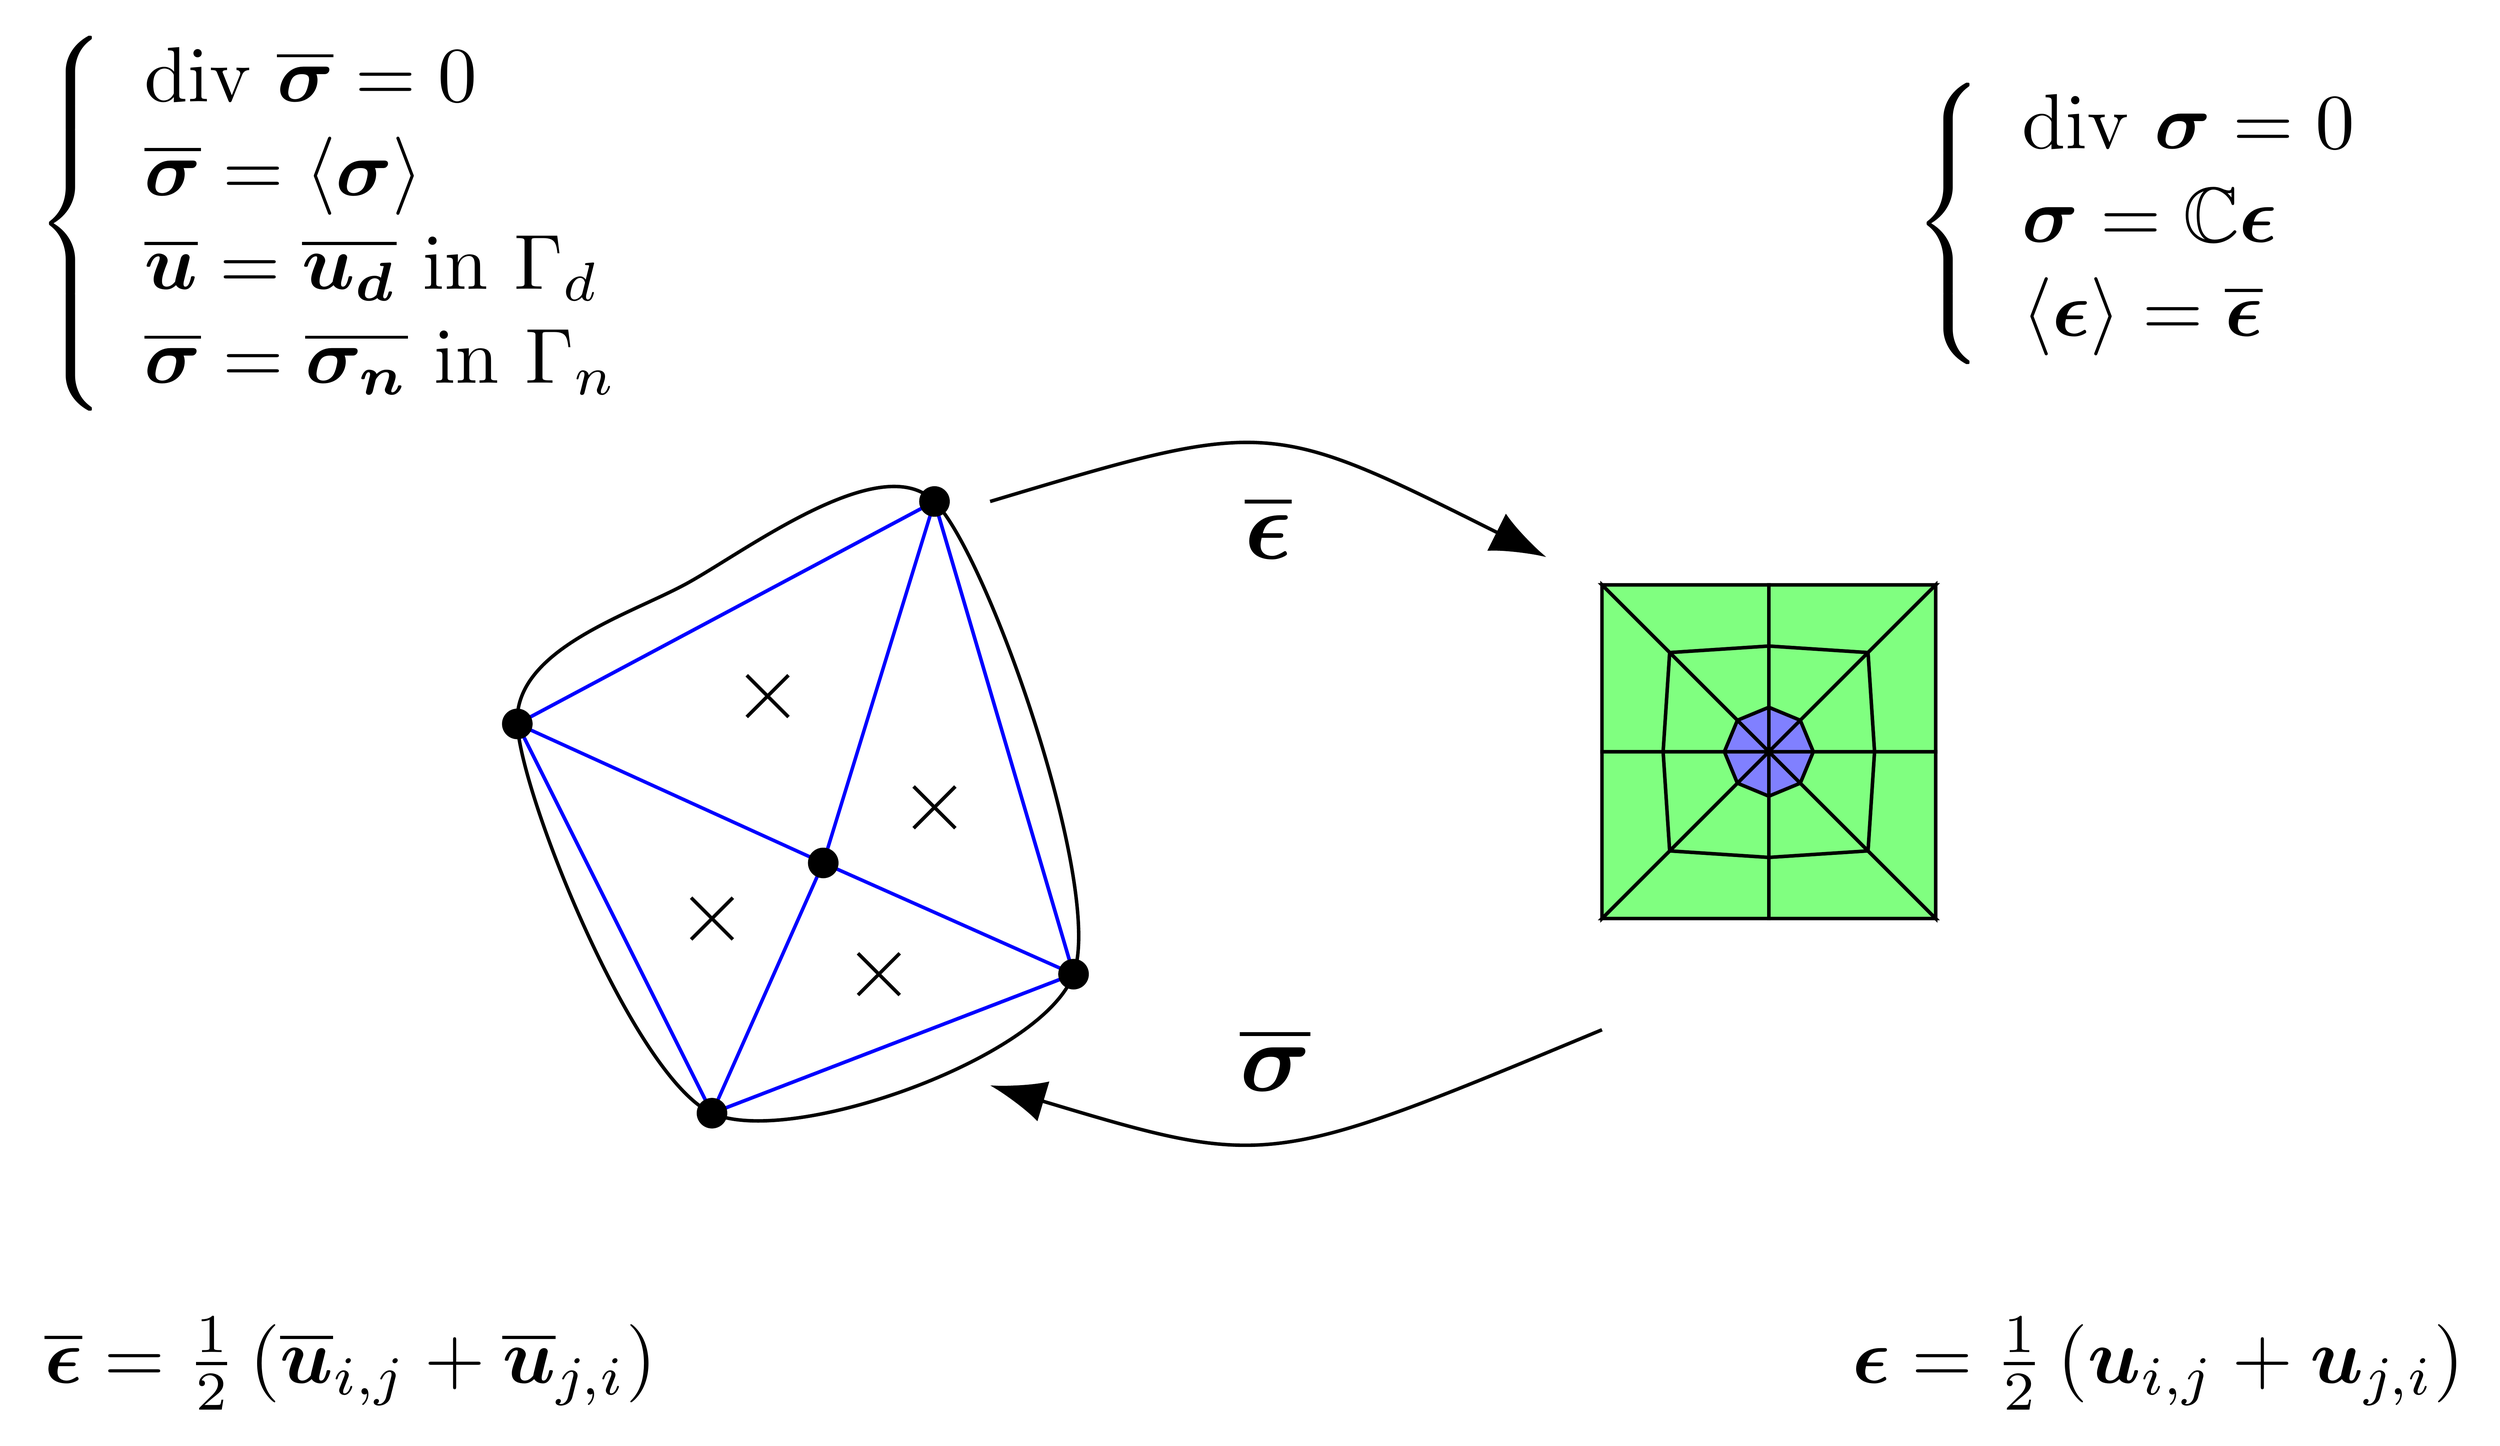
\begin{tikzpicture}[>=latex,node distance=0pt, line width=1.25mm]

% the h.m.s.

    \coordinate [draw=black,shift={(0,0)}] (0) at (6,15);
    \coordinate [draw=black,shift={(0,0)}] (1) at (13,1);
    \coordinate [draw=black,shift={(0,0)}] (2) at (26,6);
    \coordinate [draw=black,shift={(0,0)}] (3) at (21,23);
    \coordinate [draw=black,shift={(0,0)}] (4) at (17,10);
    \draw [blue]  (0) -- (1) -- (2) -- (3) -- cycle;
    \draw [blue]  (0) -- (4);
    \draw [blue]  (1) -- (4);
    \draw [blue]  (2) -- (4);
    \draw [blue]  (3) -- (4);
    \draw [blue]  (6,15) -- (13,1) -- (26,6) -- (21,23) -- cycle;
    \draw [black] plot [smooth cycle] coordinates {(6,15) (13,1) (26,6) (21,23)
    (12,20)};
    \node [fill=black, draw=none, circle, inner sep=0pt, minimum size=1.1cm,scale=1.0] at (0) {};
    \node [fill=black, draw=none, circle, inner sep=0pt, minimum size=1.1cm,scale=1.0] at (1) {};
    \node [fill=black, draw=none, circle, inner sep=0pt, minimum size=1.1cm,scale=1.0] at (2) {};
    \node [fill=black, draw=none, circle, inner sep=0pt, minimum size=1.1cm,scale=1.0] at (3) {};
    \node [fill=black, draw=none, circle, inner sep=0pt, minimum size=1.1cm,scale=1.0] at (4) {};
    \node[cross,minimum size=1.0cm,scale=1.5] (gp_0) at (13,8) {};
    \node[cross,minimum size=1.0cm,scale=1.5] (gp_0) at (15,16) {};
    \node[cross,minimum size=1.0cm,scale=1.5] (gp_0) at (19,6) {};
    \node[cross,minimum size=1.0cm,scale=1.5] (gp_0) at (21,12) {};

% the r.v.e.

    \begin{scope}[yshift = 8 cm,xshift = 45 cm,start chain=going right,scale=4.0]
      \coordinate [draw=black,shift={(0,0)}] (0) at (0,0);
      \coordinate [draw=black,shift={(0,0)}] (1) at (1.5,0);
      \coordinate [draw=black,shift={(0,0)}] (2) at (1.5,1.5);
      \coordinate [draw=black,shift={(0,0)}] (3) at (1.5,1.1);
      \coordinate [draw=black,shift={(0,0)}] (4) at (1.2171572876,1.2171572876);
      \coordinate [draw=black,shift={(0,0)}] (5) at (1.1,1.5);
      \coordinate [draw=black,shift={(0,0)}] (6) at (0,1.5);
      \coordinate [draw=black,shift={(0,0)}] (7) at (0,3);
      \coordinate [draw=black,shift={(0,0)}] (8) at (1.2171572876,1.7828427124);
      \coordinate [draw=black,shift={(0,0)}] (9) at (1.5,1.9);
      \coordinate [draw=black,shift={(0,0)}] (10) at (1.5,3);
      \coordinate [draw=black,shift={(0,0)}] (11) at (3,0);
      \coordinate [draw=black,shift={(0,0)}] (12) at (1.7828427124,1.2171572876);
      \coordinate [draw=black,shift={(0,0)}] (13) at (1.9,1.5);
      \coordinate [draw=black,shift={(0,0)}] (14) at (3,1.5);
      \coordinate [draw=black,shift={(0,0)}] (15) at (3,3);
      \coordinate [draw=black,shift={(0,0)}] (16) at (1.7828427124,1.7828427124);
      \coordinate [draw=black,shift={(0,0)}] (17) at (1.5,0.5500000000014312);
      \coordinate [draw=black,shift={(0,0)}] (18) at (0.6085786437983935,0.6085786437983935);
      \coordinate [draw=black,shift={(0,0)}] (19) at (0.5500000000014312,1.5);
      \coordinate [draw=black,shift={(0,0)}] (20) at (0.6085786437983723,2.391421356201628);
      \coordinate [draw=black,shift={(0,0)}] (21) at (1.5,2.449999999998004);
      \coordinate [draw=black,shift={(0,0)}] (22) at (2.391421356201628,0.6085786437983723);
      \coordinate [draw=black,shift={(0,0)}] (23) at (2.449999999998004,1.5);
      \coordinate [draw=black,shift={(0,0)}] (24) at (2.391421356201648,2.391421356201648);
      \draw [fill=blue!50] (2) --  (4) --  (3) -- cycle;
      \draw [fill=blue!50] (2) --  (4) --  (5) -- cycle;
      \draw [fill=blue!50] (2) --  (8) --  (9) -- cycle;
      \draw [fill=blue!50] (2) --  (8) --  (5) -- cycle;
      \draw [fill=blue!50] (2) --  (12) --  (3) -- cycle;
      \draw [fill=blue!50] (2) --  (12) --  (13) -- cycle;
      \draw [fill=blue!50] (2) --  (16) --  (9) -- cycle;
      \draw [fill=blue!50] (2) --  (16) --  (13) -- cycle;
      \draw [fill=green!50] (0) --  (18) --  (17) --  (1) -- cycle;
      \draw [fill=green!50] (18) --  (4) --  (3) --  (17) -- cycle;
      \draw [fill=green!50] (0) --  (18) --  (19) --  (6) -- cycle;
      \draw [fill=green!50] (18) --  (4) --  (5) --  (19) -- cycle;
      \draw [fill=green!50] (7) --  (20) --  (21) --  (10) -- cycle;
      \draw [fill=green!50] (20) --  (8) --  (9) --  (21) -- cycle;
      \draw [fill=green!50] (7) --  (20) --  (19) --  (6) -- cycle;
      \draw [fill=green!50] (20) --  (8) --  (5) --  (19) -- cycle;
      \draw [fill=green!50] (11) --  (22) --  (17) --  (1) -- cycle;
      \draw [fill=green!50] (22) --  (12) --  (3) --  (17) -- cycle;
      \draw [fill=green!50] (11) --  (22) --  (23) --  (14) -- cycle;
      \draw [fill=green!50] (22) --  (12) --  (13) --  (23) -- cycle;
      \draw [fill=green!50] (15) --  (24) --  (21) --  (10) -- cycle;
      \draw [fill=green!50] (24) --  (16) --  (9) --  (21) -- cycle;
      \draw [fill=green!50] (15) --  (24) --  (23) --  (14) -- cycle;
      \draw [fill=green!50] (24) --  (16) --  (13) --  (23) -- cycle;
      \node [fill=black, draw=none, circle, inner sep=0pt, minimum size=0.1cm,scale=0.3] at (0) {h};
      \node [fill=black, draw=none, circle, inner sep=0pt, minimum size=0.1cm,scale=0.3] at (1) {h};
      \node [fill=black, draw=none, circle, inner sep=0pt, minimum size=0.1cm,scale=0.3] at (2) {h};
      \node [fill=black, draw=none, circle, inner sep=0pt, minimum size=0.1cm,scale=0.3] at (3) {h};
      \node [fill=black, draw=none, circle, inner sep=0pt, minimum size=0.1cm,scale=0.3] at (4) {h};
      \node [fill=black, draw=none, circle, inner sep=0pt, minimum size=0.1cm,scale=0.3] at (5) {h};
      \node [fill=black, draw=none, circle, inner sep=0pt, minimum size=0.1cm,scale=0.3] at (6) {h};
      \node [fill=black, draw=none, circle, inner sep=0pt, minimum size=0.1cm,scale=0.3] at (7) {h};
      \node [fill=black, draw=none, circle, inner sep=0pt, minimum size=0.1cm,scale=0.3] at (8) {h};
      \node [fill=black, draw=none, circle, inner sep=0pt, minimum size=0.1cm,scale=0.3] at (9) {h};
      \node [fill=black, draw=none, circle, inner sep=0pt, minimum size=0.1cm,scale=0.3] at (10) {h};
      \node [fill=black, draw=none, circle, inner sep=0pt, minimum size=0.1cm,scale=0.3] at (11) {h};
      \node [fill=black, draw=none, circle, inner sep=0pt, minimum size=0.1cm,scale=0.3] at (12) {h};
      \node [fill=black, draw=none, circle, inner sep=0pt, minimum size=0.1cm,scale=0.3] at (13) {h};
      \node [fill=black, draw=none, circle, inner sep=0pt, minimum size=0.1cm,scale=0.3] at (14) {h};
      \node [fill=black, draw=none, circle, inner sep=0pt, minimum size=0.1cm,scale=0.3] at (15) {h};
      \node [fill=black, draw=none, circle, inner sep=0pt, minimum size=0.1cm,scale=0.3] at (16) {h};
      \node [fill=black, draw=none, circle, inner sep=0pt, minimum size=0.1cm,scale=0.3] at (17) {h};
      \node [fill=black, draw=none, circle, inner sep=0pt, minimum size=0.1cm,scale=0.3] at (18) {h};
      \node [fill=black, draw=none, circle, inner sep=0pt, minimum size=0.1cm,scale=0.3] at (19) {h};
      \node [fill=black, draw=none, circle, inner sep=0pt, minimum size=0.1cm,scale=0.3] at (20) {h};
      \node [fill=black, draw=none, circle, inner sep=0pt, minimum size=0.1cm,scale=0.3] at (21) {h};
      \node [fill=black, draw=none, circle, inner sep=0pt, minimum size=0.1cm,scale=0.3] at (22) {h};
      \node [fill=black, draw=none, circle, inner sep=0pt, minimum size=0.1cm,scale=0.3] at (23) {h};
      \node [fill=black, draw=none, circle, inner sep=0pt, minimum size=0.1cm,scale=0.3] at (24) {h};
    \end{scope}

    \draw[-{Latex[length=20mm,width=15mm]}] (23,23) ..  controls ++(10,+3) ..
    node[below, scale=10] {$\overline{\bm{\epsilon}}$} 
    ++(20,-2);
    \draw[{Latex[length=20mm,width=15mm]}-] (23,2) .. controls ++(10,-3) .. 
    node[above, scale=10] {$\overline{\bm{\sigma}}$}
    ++(22,+2);

    \node[scale=8] at (65,33) {$
    \left\{
    \begin{array}{ll}
    \text{div } \bm{\sigma} = 0 \\
    \bm{\sigma} = \mathbb{C}\bm{\epsilon} \\
    \langle \bm{\epsilon} \rangle = \overline{\bm{\epsilon}}\\
    \end{array}
    \right.
    $};

    \node[scale=8] at (0,33) {$
    \left\{
    \begin{array}{ll}
    \text{div } \overline{\bm{\sigma}} = 0 \\
    \overline{\bm{\sigma}} = \langle \bm{\sigma} \rangle \\
    \overline{\bm{u}} = \overline{\bm{u_d}} \text{ in } \Gamma_d\\
    \overline{\bm{\sigma}} = \overline{\bm{\sigma_n}} \text{ in } \Gamma_n
    \end{array}
    \right.
    $};

    \node[scale=8] at (0,-8) {$\overline{\bm{\epsilon}} = \frac{1}{2} \left(\overline{\bm{u}}_{i,j} + \overline{\bm{u}}_{j,i}\right)$};
    \node[scale=8] at (65,-8) {${\bm{\epsilon}} = \frac{1}{2} \left({\bm{u}}_{i,j} + {\bm{u}}_{j,i}\right)$};

\end{tikzpicture}

\end{document}
}
\end{figure}
\end{frame}

%------------------------------------------------

\begin{frame}
\frametitle{The FE$^2$ multi-scale method}
{\color{ForestGreen}Advantages}
\begin{itemize}
\item There is no need of construct complex constitutive micro-models, i.e., it has lot of flexibility under
micro-structure variations $\Rightarrow$ can be quicker for the design
stage of pieces.
\item It can give more accurate results than other methods.
\end{itemize}

{\color{Red}Disadvantages}
\begin{itemize}
\item Only works for problems where FEM can be applyied at both scales. For example, we can't go to the atomic scale.
\item It is generally more computationally expensive than other multi-scale methods $\Rightarrow$ It needs an efficient
design and a lot of computational power. 
\end{itemize}
\end{frame}

%------------------------------------------------

\begin{frame}
\frametitle{The distributed strategy}

\begin{figure}[!ht]
\resizebox{1.0\linewidth}{!}{\documentclass{standalone}

\begin{document}

\tikzset{cross/.style={cross out, draw=black, fill=none, minimum size=2*(#1-\pgflinewidth), inner sep=0pt, outer
sep=0pt}, cross/.default={2pt}}

\begin{tikzpicture}[node distance=4cm]

  \node[scale=.15] at (-2,6) {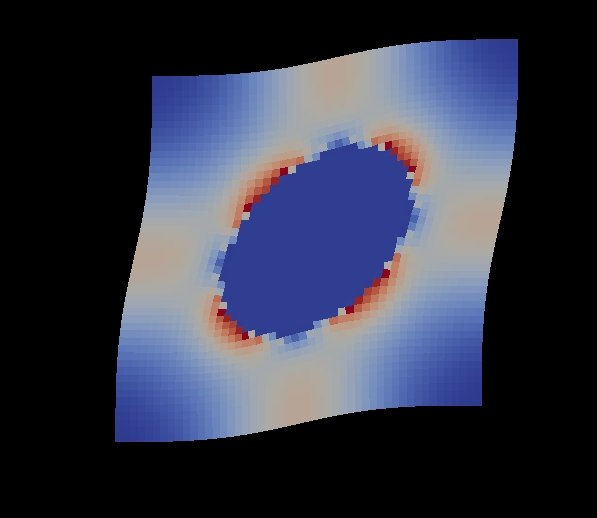
\includegraphics[]{figures/periodic_exy.jpg}};
  \draw[-{Latex[length=5mm,width=4mm]},line width=1.5mm] (-0,6) -- +(1,0);

  \tikzstyle{mpi} = [fill=red,draw=red,text=black,minimum size=1cm]
  \tikzstyle{openmp} = [fill=none,draw=red,text=black,minimum size=1cm]

  \node[] at (10,15)   {$\rightarrow$ Intel Xeon Platinum chips, 165.888 processors, 11.5 PFlops};
  \node[] at (10,14.5) {$\rightarrow$ IBM Power 9 + nVidia Volta GPUs, 1.5 PFlops};
  \node[] at (10,14)   {$\rightarrow$ Intel Knight’s Hill (KNH), 0.5 PFlops};
  \node[] at (10,13.5) {$\rightarrow$ 64-bit ARMv8 with Fujitsu technology, 0.5 Pflops};

  \node[mpi,fill=green!50] (MPI_0) at (2,10) {M$_0$};
  \node[mpi] (MPI_1) [right of = MPI_0] {M$_1$};
  \node[mpi,fill=green!50] (MPI_2) [right of = MPI_1] {M$_2$};
  \node[mpi,fill=green!50] (MPI_3) [right of = MPI_2] {M$_3$};

  \node[mpi,fill=blue!50] (MPI_4) at (2,6) {$\mu_4$};
  \node[mpi] (MPI_5) [right of = MPI_4] {$\mu_5$};
  \node[mpi,fill=blue!50] (MPI_6) [right of = MPI_5] {$\mu_6$};
  \node[mpi,fill=blue!50] (MPI_7) [right of = MPI_6] {$\mu_7$};

  \node[openmp] (OpenMP_0) [below left = 2cm and 0cm of MPI_4] {$\mu_{4,0}$};
  \node[openmp] (OpenMP_1) [below right = 2cm and 0cm of MPI_4] {$\mu_{4,1}$};
  \node[openmp] (OpenMP_2) [below left = 2cm and 0cm of MPI_5] {$\mu_{5,0}$};
  \node[openmp] (OpenMP_3) [below right = 2cm and 0cm of MPI_5] {$\mu_{5,1}$};
  \node[openmp] (OpenMP_4) [below left = 2cm and 0cm of MPI_6] {$\mu_{6,0}$};
  \node[openmp] (OpenMP_5) [below right = 2cm and 0cm of MPI_6] {$\mu_{6,1}$};
  \node[openmp] (OpenMP_6) [below left = 2cm and 0cm of MPI_7] {$\mu_{7,0}$};
  \node[openmp] (OpenMP_7) [below right = 2cm and 0cm of MPI_7] {$\mu_{7,1}$};

  \node[draw,fill=none] [above right = 0.5cm and -2.5cm of OpenMP_4] {OpenMP};
  \node[draw,fill=none] [above right = 7.0cm and -2.2cm of OpenMP_4] {MPI};
  \node[draw,fill=none] [above right = 7.0cm and -6.0cm of OpenMP_4] {MPI};
  \node[draw,fill=none] [above right = 7.0cm and +2.0cm of OpenMP_4] {MPI};

  \draw [draw=red,dashed,line width = 2mm, -] (MPI_0) -- (MPI_1);
  \draw [draw=red,dashed,line width = 2mm,-] (MPI_1) -- (MPI_2);
  \draw [draw=red,dashed,line width = 2mm,-] (MPI_2) -- (MPI_3);

  \draw [draw=red,-] (MPI_0) -- (MPI_4);
  \draw [draw=red,-] (MPI_1) -- (MPI_5);
  \draw [draw=red,-] (MPI_2) -- (MPI_6);
  \draw [draw=red,-] (MPI_3) -- (MPI_7);

  \draw [draw=red,-,dashed] (MPI_4) -- (OpenMP_0);
  \draw [draw=red,-,dashed] (MPI_4) -- (OpenMP_1);

  \draw [draw=red,-,dashed] (MPI_5) -- (OpenMP_2);
  \draw [draw=red,-,dashed] (MPI_5) -- (OpenMP_3);

  \draw [draw=red,-,dashed] (MPI_6) -- (OpenMP_4);
  \draw [draw=red,-,dashed] (MPI_6) -- (OpenMP_5);

  \draw [draw=red,-,dashed] (MPI_7) -- (OpenMP_6);
  \draw [draw=red,-,dashed] (MPI_7) -- (OpenMP_7);

  \draw[-{Latex[length=5mm,width=4mm]},line width=1.5mm,black] (0,14) ..  controls ++(5,0) .. (6,11);

  \begin{scope}[xshift=2cm,yshift=5cm]
   \node[fill=none, draw=red, minimum size = 2cm] (square_0) at (-6,8) {};
   \node[fill=red, draw=red, minimum size = 2cm] (square_1) at (-4,8) {};
   \node[fill=none, draw=red, minimum size = 2cm] (square_2) at (-6,6) {};
   \node[fill=none, draw=red, minimum size = 2cm] (square_3) at (-4,6) {};

   \node[circle,fill=black, draw=black, minimum size = 0.05cm] (node_0) at (-5,9) {};
   \node[circle,fill=black, draw=black, minimum size = 0.05cm] (node_1) at (-4,9) {};
   \node[circle,fill=black, draw=black, minimum size = 0.05cm] (node_2) at (-3,9) {};
   \node[circle,fill=black, draw=black, minimum size = 0.05cm] (node_3) at (-5,8) {};
   \node[circle,fill=black, draw=black, minimum size = 0.05cm] (node_4) at (-4,8) {};
   \node[circle,fill=black, draw=black, minimum size = 0.05cm] (node_5) at (-3,8) {};
   \node[circle,fill=black, draw=black, minimum size = 0.05cm] (node_6) at (-5,7) {};
   \node[circle,fill=black, draw=black, minimum size = 0.05cm] (node_7) at (-4,7) {};
   \node[circle,fill=black, draw=black, minimum size = 0.05cm] (node_8) at (-3,7) {};

   \draw [draw=black,-] (-5,9) -- (-3,9);
   \draw [draw=black,-] (-5,8) -- (-3,8);
   \draw [draw=black,-] (-5,7) -- (-3,7);

   \draw [draw=black,-] (-5,9) -- (-5,7);
   \draw [draw=black,-] (-4,9) -- (-4,7);
   \draw [draw=black,-] (-3,9) -- (-3,7);

   \node[fill=none, draw=none] (title_1) at (-2,8) {M$_i$};

   \node[cross,minimum size=0.2cm] (gp_0) at (-4.5,8.5) {};
   \node[cross,minimum size=0.2cm] (gp_1) at (-3.5,8.5) {};
   \node[cross,minimum size=0.2cm] (gp_2) at (-4.5,7.5) {};
   \node[cross,minimum size=0.2cm] (gp_3) at (-3.5,7.5) {};
  \end{scope}
 \end{tikzpicture}

\end{document}
}
\end{figure}
\end{frame}

%------------------------------------------------

\begin{frame}
\frametitle{Microscopic code design}

\begin{figure}[!ht]
\resizebox{1.0\linewidth}{!}{
\begin{tikzpicture}[node distance=4cm]
    \node[inner sep=0pt, scale=0.1] (rve) at (0,0) {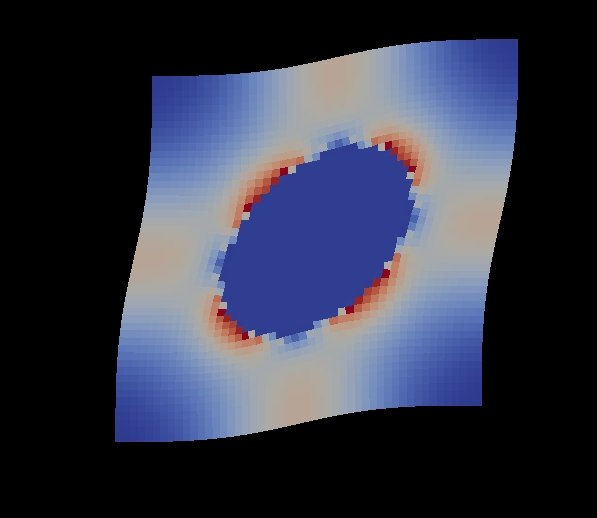
\includegraphics[width=1.4\textwidth]{figures/periodic_exy.jpg}};
    \node[inner sep=0pt, scale=1.0] (rve) at (3,0) {$t_{calc} \approx \#_{gp} \times t_{micro} $};
\end{tikzpicture}
}
\end{figure}

\end{frame}

%------------------------------------------------

\begin{frame}
\frametitle{Microscopic code design}

\textcolor{OliveGreen}{Constrains and approximations} :
\begin{itemize}
  \item will use structured grids :
  \begin{itemize}
   \item more data locality : for matrices and variables at integration points $\Rightarrow$ less cache misses.
   \item periodic and uniform stress boundary conditions are easier to implement.
  \end{itemize}
  \item will run on one node architecture, one code in \textbf{one} multi-core processor or \textbf{one} GPU.
  \begin{itemize}
   \item easy to communicate and to couple with a macroscopic master code (\textbf{Alya}).
   \item flexible for running on most common supercomputers such us \textbf{Marenostrum}.
  \end{itemize}

\end{itemize}

\begin{figure}[!ht]
\resizebox{0.3\linewidth}{!}{
\begin{tikzpicture}[node distance=4cm]
    \node[inner sep=0pt, scale=0.1] (rve) at (0,0) {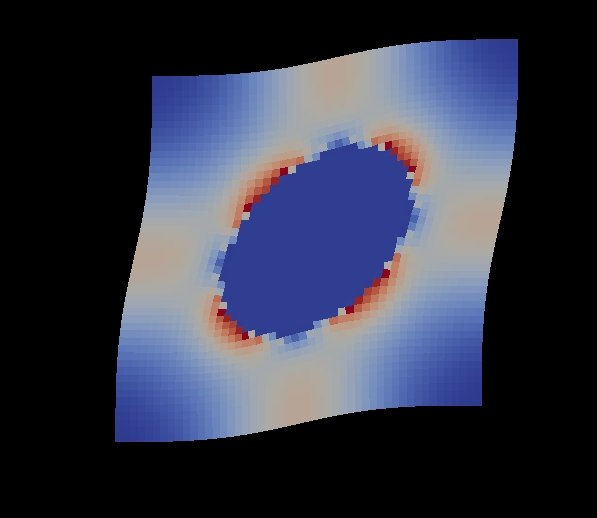
\includegraphics[width=1.4\textwidth]{figures/periodic_exy.jpg}};
\end{tikzpicture}
}
\end{figure}

\end{frame}

%------------------------------------------------

\begin{frame}
\frametitle{Validation FE$^2$ problem}
\begin{figure}[!ht]
\resizebox{0.8\linewidth}{!}{\documentclass{standalone}

\begin{document}

\begin{tikzpicture}[node distance=4cm]

    \node[inner sep=0pt, scale=0.1] (rve) at (0,0) {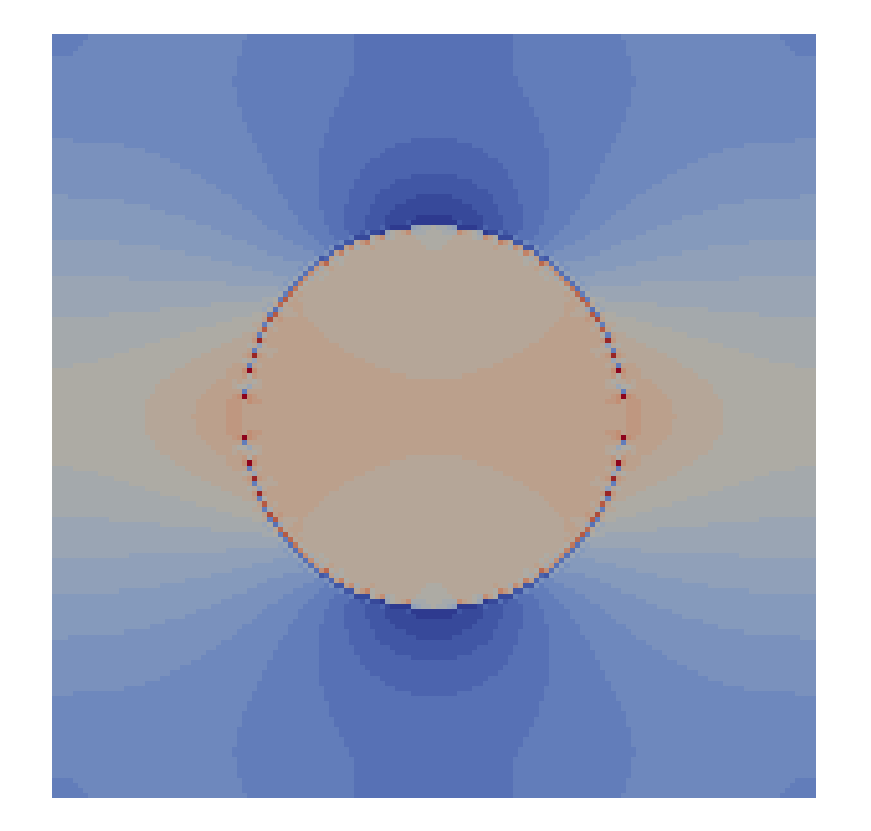
\includegraphics[width=1.4\textwidth]{figures/front_exp_0-crop.pdf}};
    \node[inner sep=0pt, scale=0.1] (rve) at (2,0) {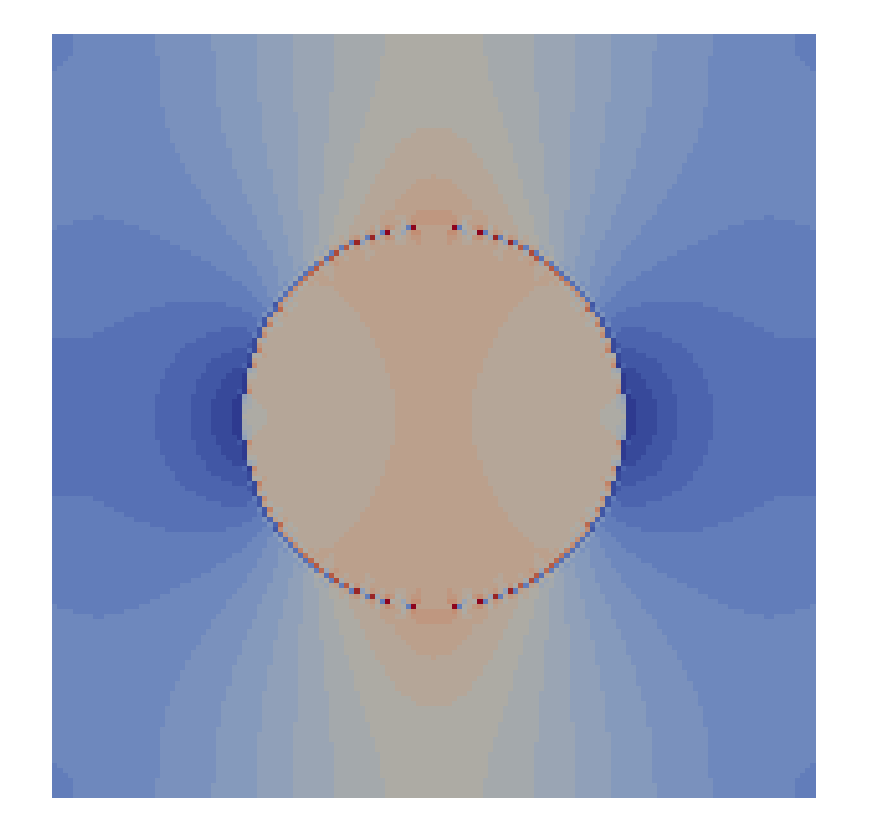
\includegraphics[width=1.4\textwidth]{figures/front_exp_1-crop.pdf}};
    \node[inner sep=0pt, scale=0.1] (rve) at (4,0) {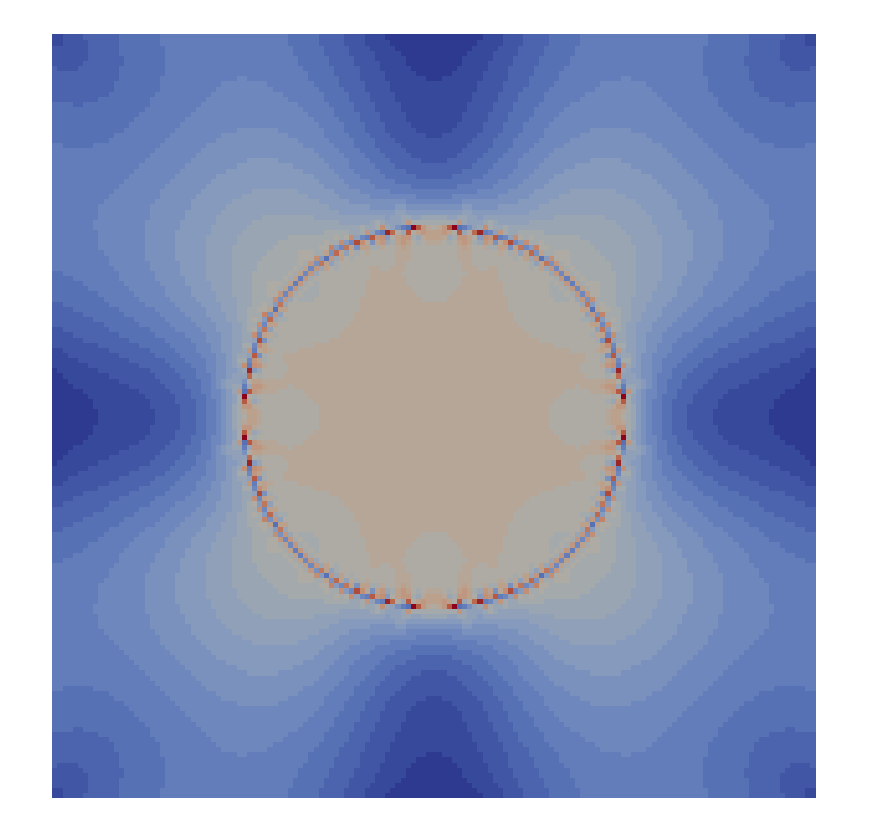
\includegraphics[width=1.4\textwidth]{figures/front_exp_2-crop.pdf}};
    \node[inner sep=0pt, scale=0.25] (rve) at (2,2.2) {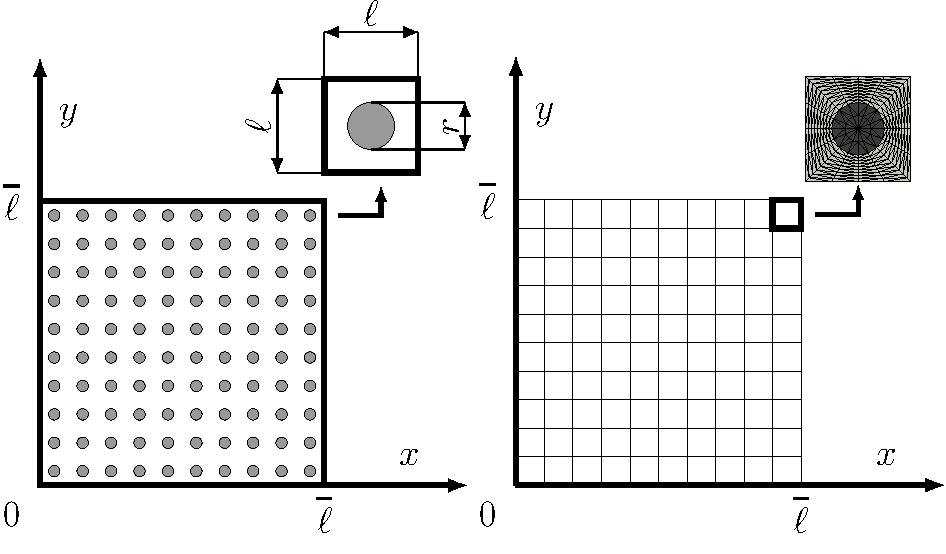
\includegraphics[width=1.4\textwidth]{figures/prob_paper_2.pdf}};

\end{tikzpicture}

\end{document}
}
\end{figure}
\end{frame}

%------------------------------------------------

\begin{frame}
\frametitle{Validation FE$^2$ problem}
\begin{figure}[!ht]
\resizebox{1.0\linewidth}{!}{\documentclass{standalone}

\begin{document}

\begin{tikzpicture}[node distance=4cm]

    \node[inner sep=0pt, scale=0.3] at (0,0) {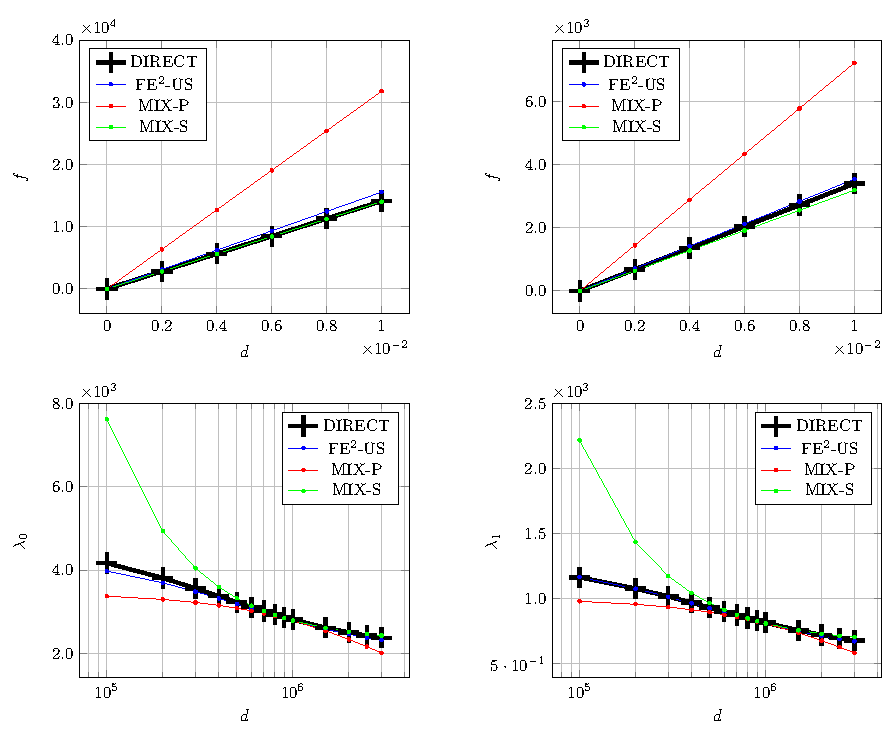
\includegraphics[width=1.4\textwidth]{figures/res_paper_2.pdf}};
    \node[inner sep=0pt, scale=0.1] at (4,1) {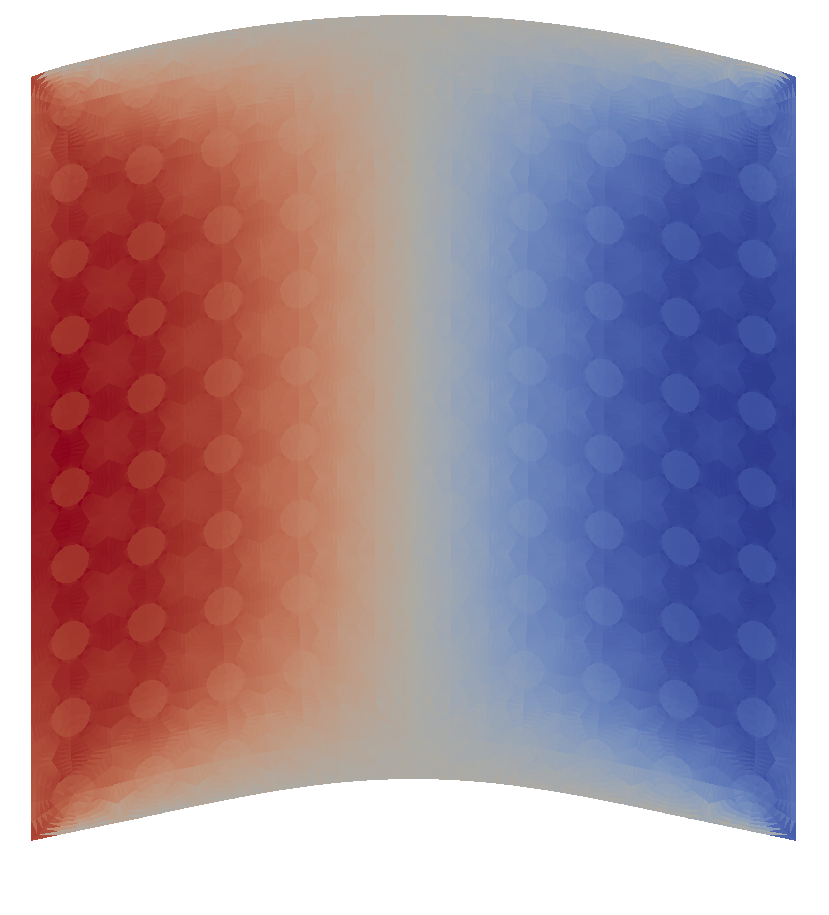
\includegraphics[width=1.4\textwidth]{figures/fig_direct-crop.pdf}};
    \node[inner sep=0pt, scale=0.1] at (4,-1) {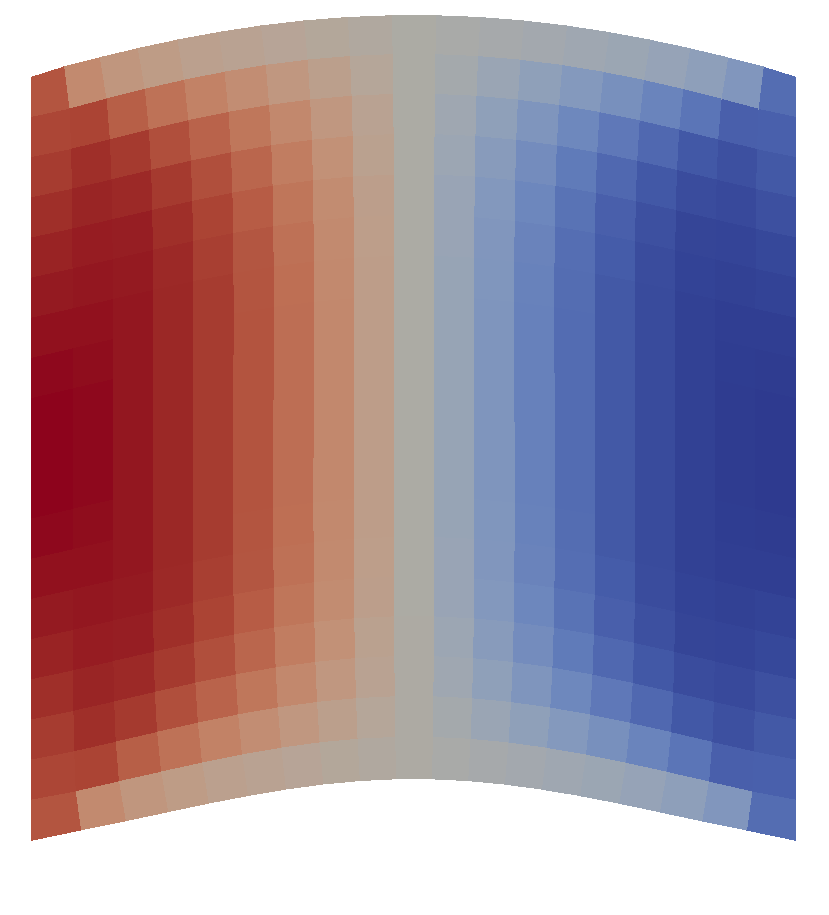
\includegraphics[width=1.4\textwidth]{figures/fig_homog_us-crop.pdf}};

 \end{tikzpicture}

\end{document}
}
\end{figure}
\end{frame}

%------------------------------------------------

\begin{frame}
\frametitle{Periodic BC case}

\begin{tikzpicture}[node distance=4cm]
    \node[inner sep=0pt, scale=1] (rve) at (0,0) {
     $\left\{
     \begin{array}{ll}
     \bm{f}_a(\bm{u}) = \bm{0} \\
     \bm{f}_b^+(\bm{u}) + \bm{f}_b^-(\bm{u}) = \bm{0} \\
     \bm{u}^+ - \bm{u}^- - \overline{\bm{\epsilon}} ( \bm{x}^+ - \bm{x}^- ) = \bm{0}\\
     \end{array}
     \right.$
      };
    \node[inner sep=0pt, scale=0.2] (rve) at (6,0) {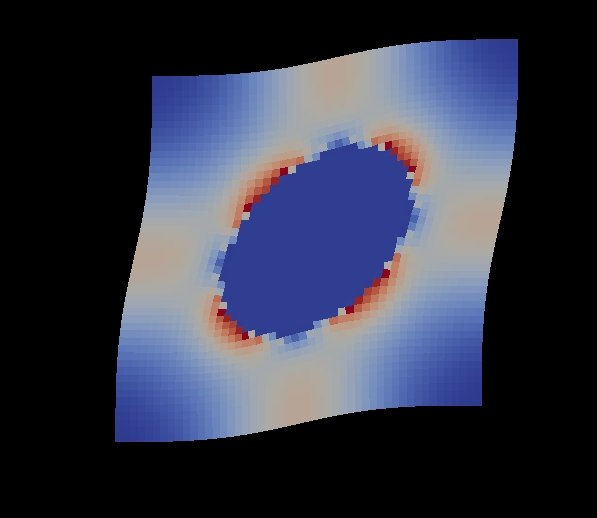
\includegraphics[width=1.4\textwidth]{figures/periodic_exy.jpg}};
\end{tikzpicture}

\vspace{.4cm}
Unknowns elimination
\vspace{.4cm}

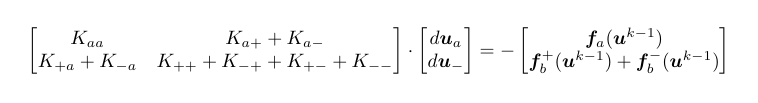
\begin{tikzpicture}[node distance=4cm]
    \node[inner sep=0pt, scale=0.7] (rve) at (0,0) {$
     \begin{bmatrix}
     K_{aa}          & K_{a+} + K_{a-} \\
     K_{+a} + K_{-a} & K_{++} + K_{-+}  + K_{+-} + K_{--} \\
     \end{bmatrix}
     \cdot
     \begin{bmatrix}d\bm{u}_a \\ d\bm{u}_- \end{bmatrix}
     =
     -\begin{bmatrix}\bm{f}_a(\bm{u}^{k-1}) \\ \bm{f}_b^+(\bm{u}^{k-1}) + \bm{f}_b^-(\bm{u}^{k-1}) \end{bmatrix}
    $};
\end{tikzpicture}

\vspace{.4cm}
Lagrange multipliers
\vspace{.4cm}

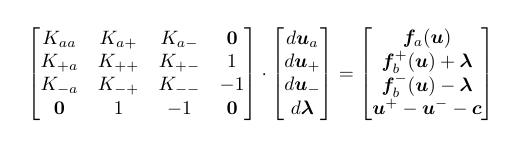
\begin{tikzpicture}[node distance=4cm]
    \node[inner sep=0pt, scale=0.7] (rve) at (0,1) {$
    \begin{bmatrix}
    K_{aa} & K_{a+} & K_{a-} &  \bm{0}\\
    K_{+a} & K_{++} & K_{+-} &  \mathbbm{1}\\
    K_{-a} & K_{-+} & K_{--} & -\mathbbm{1}\\
    \bm{0}                                    & \mathbbm{1}                               & -\mathbbm{1}                              &  \bm{0}\\
    \end{bmatrix}
    \cdot
    \begin{bmatrix}
    d\bm{u}_a \\
    d\bm{u}_+ \\
    d\bm{u}_- \\
    d\bm{\lambda}
    \end{bmatrix}
    =
    \begin{bmatrix}
    \bm{f}_a(\bm{u}) \\
    \bm{f}_b^+(\bm{u}) + \bm{\lambda} \\
    \bm{f}_b^-(\bm{u}) - \bm{\lambda} \\
    \bm{u}^{+} - \bm{u}^{-} - \bm{c}
    \end{bmatrix}
    $};
\end{tikzpicture}

\end{frame}

%------------------------------------------------

\begin{frame}
\frametitle{Periodic BC case}

Unknowns elimination
\vspace{.4cm}

\begin{tikzpicture}[node distance=4cm]
    \node[inner sep=0pt, scale=0.7] (rve) at (-0.3,0) {$
     \begin{bmatrix}
     K_{aa}          & K_{a+} + K_{a-} \\
     K_{+a} + K_{-a} & K_{++} + K_{-+}  + K_{+-} + K_{--} \\
     \end{bmatrix}
     \cdot
     \begin{bmatrix}d\bm{u}_a \\ d\bm{u}_- \end{bmatrix}
     =
     -\begin{bmatrix}\bm{f}_a(\bm{u}^{k-1}) \\ \bm{f}_b^+(\bm{u}^{k-1}) + \bm{f}_b^-(\bm{u}^{k-1}) \end{bmatrix}
    $};
    \node[inner sep=0pt, scale=0.1] (rve) at (5.5,0) {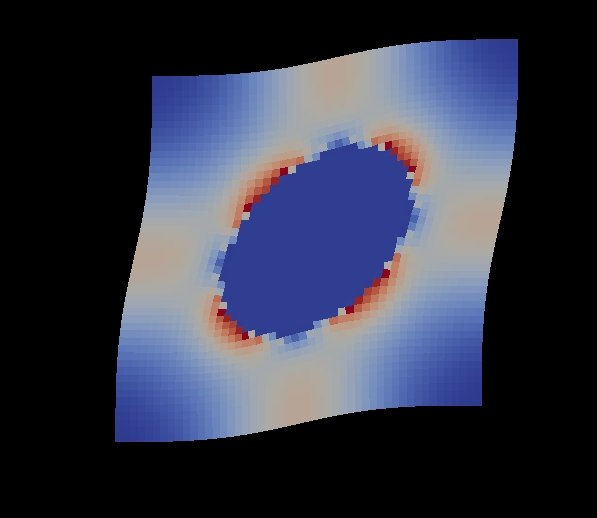
\includegraphics[width=1.4\textwidth]{figures/periodic_exy.jpg}};
    \pgfplotstableread{figures/cg.dat}{\cg}
    \pgfplotstableread{figures/cg_pd.dat}{\cgpd}
    \begin{axis}[
      xlabel=problem size,ylabel=time,
      tick scale binop=\times,
      y tick label style={/pgf/number format/.cd, set thousands separator={}, 1000 sep={}, precision=1, /tikz/.cd},
      grid=both,
      legend pos=north west,
      at={(2cm,-4cm)},
      scale=0.5
    ]  
    \addplot+[mark=*,mark options={scale=0.5},color=red  ] table [x index=0, y index=1] {\cg};\addlegendentry{CG};
    \addplot+[mark=*,mark options={scale=0.5},color=green] table [x index=0, y index=1] {\cgpd};\addlegendentry{CG-PD};
    \end{axis}
    \begin{axis}[
      xlabel=problem size,ylabel=iterations,
      tick scale binop=\times,
      y tick label style={/pgf/number format/.cd, 1000 sep={}, precision=1, /tikz/.cd},
      grid=both,
      legend pos=north west,
      at={(-4cm,-4cm)},
      scale=0.5
    ]  
    \addplot+[mark=*,mark options={scale=0.5},color=red  ] table [x index=0, y index=2] {\cg};\addlegendentry{CG};
    \addplot+[mark=*,mark options={scale=0.5},color=green] table [x index=0, y index=2] {\cgpd};\addlegendentry{CG-PD};
    \end{axis}
\end{tikzpicture}

\end{frame}

%----------------------------------------------------------------------------------------

\begin{frame}
\frametitle{Working Plan}

\begin{itemize}
\item \textcolor{OliveGreen}{Short term goal} : \textbf{Search for an efficient implementation of the microscopic code}. 
 For each boundary condition type and algorithm test :
 \begin{itemize}
  \item different solvers (pre-conditioners) and matrix storage formats.
  \item different architectures and parallelization strategies.
 \end{itemize}

 \item \textcolor{Red}{Long term goal}: Solve a large problem with \textbf{Alya} :
 \begin{itemize}
  \item couple the microscopic code with \textbf{Alya}.
  \item solve a real size non-linear problem :
  \begin{itemize}
  \item \textbf{10-100 millions elements} (macroscopic scale) 
  \item \textbf{0.1-1 millions elements} (microscopic scale) 
  \item using up to \textbf{100,000 cores}.
  \end{itemize}
 \end{itemize}
\end{itemize}

\begin{figure}[hhh!]
\begin{center}
\resizebox{10cm}{!}{

\begin{ganttchart}[vgrid, hgrid]{1}{36}
\gantttitle{2017}{12} 
\gantttitle{2018}{12}
\gantttitle{2019}{12}\\
\gantttitlelist{1,...,36}{1}\\

\ganttgroup{Training}{1}{5}\\

\ganttbar[bar/.append style={fill=green}]{microscopic code}{6}{24} \\

\ganttbar[bar/.append style={fill=red}]{coupling with Alya}{25}{29} \\
\ganttbar[bar/.append style={fill=red}]{solve large problem}{27}{36} \\

\ganttgroup{Thesis}{30}{36}

\end{ganttchart}
}
\end{center}
\end{figure}

\end{frame}

%----------------------------------------------------------------------------------------

\begin{frame}
\frametitle{Proyects Involved}
\begin{itemize}
\item \textcolor{OliveGreen}{SHERLOC}: \textit{Structural health monitoring, manufacturing and repair technologies for life management of composite fuselage}
\vspace{1cm}
\item SILICOFCM : \textit{In Silico trials for drug tracing the effects of sarcomeric protein mutations leading to familial cardiomyopathy}
\item IBM-BSC : \textit{Multi-physics/Multi-scale Simulations in Heterogeneous Supercomputing Architectures.}
\end{itemize}
\end{frame}

%------------------------------------------------

\end{document} 
